\documentclass[twoside]{book}

% Packages required by doxygen
\usepackage{fixltx2e}
\usepackage{calc}
\usepackage{doxygen}
\usepackage[export]{adjustbox} % also loads graphicx
\usepackage{graphicx}
\usepackage[utf8]{inputenc}
\usepackage{makeidx}
\usepackage{multicol}
\usepackage{multirow}
\PassOptionsToPackage{warn}{textcomp}
\usepackage{textcomp}
\usepackage[nointegrals]{wasysym}
\usepackage[table]{xcolor}

% Font selection
\usepackage[T1]{fontenc}
\usepackage[scaled=.90]{helvet}
\usepackage{courier}
\usepackage{amssymb}
\usepackage{sectsty}
\renewcommand{\familydefault}{\sfdefault}
\allsectionsfont{%
  \fontseries{bc}\selectfont%
  \color{darkgray}%
}
\renewcommand{\DoxyLabelFont}{%
  \fontseries{bc}\selectfont%
  \color{darkgray}%
}
\newcommand{\+}{\discretionary{\mbox{\scriptsize$\hookleftarrow$}}{}{}}

% Page & text layout
\usepackage{geometry}
\geometry{%
  a4paper,%
  top=2.5cm,%
  bottom=2.5cm,%
  left=2.5cm,%
  right=2.5cm%
}
\tolerance=750
\hfuzz=15pt
\hbadness=750
\setlength{\emergencystretch}{15pt}
\setlength{\parindent}{0cm}
\setlength{\parskip}{3ex plus 2ex minus 2ex}
\makeatletter
\renewcommand{\paragraph}{%
  \@startsection{paragraph}{4}{0ex}{-1.0ex}{1.0ex}{%
    \normalfont\normalsize\bfseries\SS@parafont%
  }%
}
\renewcommand{\subparagraph}{%
  \@startsection{subparagraph}{5}{0ex}{-1.0ex}{1.0ex}{%
    \normalfont\normalsize\bfseries\SS@subparafont%
  }%
}
\makeatother

% Headers & footers
\usepackage{fancyhdr}
\pagestyle{fancyplain}
\fancyhead[LE]{\fancyplain{}{\bfseries\thepage}}
\fancyhead[CE]{\fancyplain{}{}}
\fancyhead[RE]{\fancyplain{}{\bfseries\leftmark}}
\fancyhead[LO]{\fancyplain{}{\bfseries\rightmark}}
\fancyhead[CO]{\fancyplain{}{}}
\fancyhead[RO]{\fancyplain{}{\bfseries\thepage}}
\fancyfoot[LE]{\fancyplain{}{}}
\fancyfoot[CE]{\fancyplain{}{}}
\fancyfoot[RE]{\fancyplain{}{\bfseries\scriptsize Generated by Doxygen }}
\fancyfoot[LO]{\fancyplain{}{\bfseries\scriptsize Generated by Doxygen }}
\fancyfoot[CO]{\fancyplain{}{}}
\fancyfoot[RO]{\fancyplain{}{}}
\renewcommand{\footrulewidth}{0.4pt}
\renewcommand{\chaptermark}[1]{%
  \markboth{#1}{}%
}
\renewcommand{\sectionmark}[1]{%
  \markright{\thesection\ #1}%
}

% Indices & bibliography
\usepackage{natbib}
\usepackage[titles]{tocloft}
\setcounter{tocdepth}{3}
\setcounter{secnumdepth}{5}
\makeindex

% Hyperlinks (required, but should be loaded last)
\usepackage{ifpdf}
\ifpdf
  \usepackage[pdftex,pagebackref=true]{hyperref}
\else
  \usepackage[ps2pdf,pagebackref=true]{hyperref}
\fi
\hypersetup{%
  colorlinks=true,%
  linkcolor=blue,%
  citecolor=blue,%
  unicode%
}

% Custom commands
\newcommand{\clearemptydoublepage}{%
  \newpage{\pagestyle{empty}\cleardoublepage}%
}

\usepackage{caption}
\captionsetup{labelsep=space,justification=centering,font={bf},singlelinecheck=off,skip=4pt,position=top}

%===== C O N T E N T S =====

\begin{document}

% Titlepage & ToC
\hypersetup{pageanchor=false,
             bookmarksnumbered=true,
             pdfencoding=unicode
            }
\pagenumbering{alph}
\begin{titlepage}
\vspace*{7cm}
\begin{center}%
{\Large Jan Of Empires }\\
\vspace*{1cm}
{\large Generated by Doxygen 1.8.14}\\
\end{center}
\end{titlepage}
\clearemptydoublepage
\pagenumbering{roman}
\tableofcontents
\clearemptydoublepage
\pagenumbering{arabic}
\hypersetup{pageanchor=true}

%--- Begin generated contents ---
\chapter{Jan of Empires Deluxe Edition}
\label{index}\hypertarget{index}{}Simple Strategy game

\section*{Ideia do jogo}

É um jogo de estratégia em turnos onde você controla 3 unidades para explorar, adquirir recursos, aumentar o poder da sua unidade usando os pilares para vencer o oponente. Cada tipo de unidade tem vantagem sobre outra unidade. O jogo é single-\/player com 1 C\+PU de oponente.

\section*{Elementos do Jogo}

\subsection*{Recursos}

Os recursos servem para criar pilares novos, criar necromancers (a partir de pilares) ou aumentar o poder de necromancers

Dois tipos de recursos\+:
\begin{DoxyItemize}
\item \mbox{\hyperlink{class_metal}{Metal}}\+: para criação de pilares. Menos abundante no mapa (terá o suficiente para criar mais 2 pilares para cada jogador).
\item \mbox{\hyperlink{class_ossos}{Ossos}}\+: para aumento de poder das unidades. Mais abundante no mapa.
\end{DoxyItemize}

\subsection*{Prédios (Pilares)}

Os prédios são pilares. Cada pilar representa uma fábrica de um tipo de unidade que será criada a partir da quantidade de ossos. Cada pilar cria uma única unidade, que é o necromancer. Depois de criado o necromancer, o pilar pode aumentar o poder do necromancer utilizando ossos.

Cada pilar tem\+:
\begin{DoxyItemize}
\item HP\+: representa a vida do pilar. Se chega a zero, ele é destruído.
\end{DoxyItemize}

É possível reconstruir pilares, com o máximo de 3 por jogador.

Três tipos de pilares\+:
\begin{DoxyItemize}
\item \mbox{\hyperlink{class_pilar}{Pilar}} da Espada\+: é o pilar que cria o necromancer guerreiro.
\item \mbox{\hyperlink{class_pilar}{Pilar}} da Lança\+: é o pilar que cria o necromancer cavaleiro.
\item \mbox{\hyperlink{class_pilar}{Pilar}} do Arco \+: é o pilar que cria o necromancer arqueiro.
\end{DoxyItemize}

\subsection*{Unidades (Necromancers)}

As unidades são representadas por um único elemento, o \mbox{\hyperlink{class_necromancer}{Necromancer}}. Cada necromancer tem um número associado que define quanto de poder ele tem. Por exemplo\+: no mapa há uma unidade A com o número 20. Isso significa que a unidade A tem 20 de poder.

Cada unidade tem\+:
\begin{DoxyItemize}
\item MP\+: representa quanto de poder a unidade tem e representa a vida da unidade. Se ela chegar a zero, a unidade morre.
\end{DoxyItemize}

São 3 tipos de unidades\+:


\begin{DoxyItemize}
\item \mbox{\hyperlink{class_necromancer}{Necromancer}} \mbox{\hyperlink{class_guerreiro}{Guerreiro}} (A)\+: é o necromancer que invoca somente undeads guerreiros. A quantidade de undeads é o que define o poder do necromancer (é o número que mostra a força da unidade). Ele tem vantagem sobre o \mbox{\hyperlink{class_necromancer}{Necromancer}} \mbox{\hyperlink{class_cavaleiro}{Cavaleiro}} e desvantagem sobre o \mbox{\hyperlink{class_necromancer}{Necromancer}} \mbox{\hyperlink{class_arqueiro}{Arqueiro}}.
\item \mbox{\hyperlink{class_necromancer}{Necromancer}} \mbox{\hyperlink{class_cavaleiro}{Cavaleiro}} (B)\+: é o necromancer que invoca somente undeads cavaleiros. A quantidade de undeads é o que define o poder do necromancer (é o número que mostra a força da unidade). Ele tem vantagem sobre o \mbox{\hyperlink{class_necromancer}{Necromancer}} \mbox{\hyperlink{class_arqueiro}{Arqueiro}} e desvantagem sobre o \mbox{\hyperlink{class_necromancer}{Necromancer}} \mbox{\hyperlink{class_guerreiro}{Guerreiro}}.
\item \mbox{\hyperlink{class_necromancer}{Necromancer}} \mbox{\hyperlink{class_arqueiro}{Arqueiro}} (C)\+: é o necromancer que invoca somente undeads arqueiros. EA quantidade de undeads é o que define o poder do necromancer (é o número que mostra a força da unidade). Ele tem vantagem sobre o \mbox{\hyperlink{class_necromancer}{Necromancer}} \mbox{\hyperlink{class_guerreiro}{Guerreiro}} e desvantagem sobre o \mbox{\hyperlink{class_necromancer}{Necromancer}} \mbox{\hyperlink{class_cavaleiro}{Cavaleiro}}.
\end{DoxyItemize}

O máximo de unidades no jogo são 6.

\section*{Regras definidas para o jogo}

\subsection*{Inicialização}

Inicialmente cada jogardor possui\+:
\begin{DoxyItemize}
\item 1 \mbox{\hyperlink{class_pilar}{Pilar}} da Espada
\item 1 \mbox{\hyperlink{class_necromancer}{Necromancer}} guerreiro
\end{DoxyItemize}

\subsection*{Turno}

Em UM turno o jogador pode criar pilares, fortalecer unidades e mover apenas uma delas. Ele acaba quando o jogador move uma peça ou decide terminar o turno.

\subsection*{Captação de recursos}

Os recursos são espalhados randômicamente no mapa no início do jogo. São capturados quando o jogador move uma unidade para o mesmo bloco em que o recurso está inserido.

\subsection*{Combate}

O combate acontece automaticamente quando duas unidades estão vizinhas O combate acontece sempre entre apenas duas unidades No combate, verificam-\/se os poderes de cada unidade, e as capacidades e fraquezas de cada uma em relação a outra, de acordo com os seus tipos. Então, é decrescido poder de cada uma de acordo com o estabelecido.

\subsection*{Condições de término do jogo}

As condições para o término do jogo são os seguintes\+:
\begin{DoxyItemize}
\item Se todos os pilares do oponente forem destruídos;
\item Se todos os recursos do mapa acabarem\+: nesse caso, a quantidade da vida dos pilares + unidades é somado. Quem tiver mais, vence.
\end{DoxyItemize}

\section*{Useful links}


\begin{DoxyItemize}
\item \href{http://lazyfoo.net/tutorials/SDL/}{\tt S\+DL Tutorial link}
\item \href{https://www.libsdl.org/release/SDL-1.2.15/docs/html/}{\tt Bibliotecas de S\+DL} 
\end{DoxyItemize}
\chapter{Hierarchical Index}
\section{Class Hierarchy}
This inheritance list is sorted roughly, but not completely, alphabetically\+:\begin{DoxyCompactList}
\item \contentsline{section}{Bloco}{\pageref{class_bloco}}{}
\item \contentsline{section}{Button}{\pageref{class_button}}{}
\item \contentsline{section}{Colocavel\+Em\+Bloco}{\pageref{class_colocavel_em_bloco}}{}
\begin{DoxyCompactList}
\item \contentsline{section}{Necromancer}{\pageref{class_necromancer}}{}
\begin{DoxyCompactList}
\item \contentsline{section}{Arqueiro}{\pageref{class_arqueiro}}{}
\item \contentsline{section}{Cavaleiro}{\pageref{class_cavaleiro}}{}
\item \contentsline{section}{Guerreiro}{\pageref{class_guerreiro}}{}
\end{DoxyCompactList}
\item \contentsline{section}{Pilar}{\pageref{class_pilar}}{}
\begin{DoxyCompactList}
\item \contentsline{section}{Pilar\+Arco}{\pageref{class_pilar_arco}}{}
\item \contentsline{section}{Pilar\+Espada}{\pageref{class_pilar_espada}}{}
\item \contentsline{section}{Pilar\+Lanca}{\pageref{class_pilar_lanca}}{}
\end{DoxyCompactList}
\item \contentsline{section}{Recurso}{\pageref{class_recurso}}{}
\begin{DoxyCompactList}
\item \contentsline{section}{Metal}{\pageref{class_metal}}{}
\item \contentsline{section}{Ossos}{\pageref{class_ossos}}{}
\end{DoxyCompactList}
\end{DoxyCompactList}
\item \contentsline{section}{Controlador}{\pageref{class_controlador}}{}
\item \contentsline{section}{Graphics}{\pageref{class_graphics}}{}
\item \contentsline{section}{Mapa}{\pageref{class_mapa}}{}
\item \contentsline{section}{Player}{\pageref{class_player}}{}
\end{DoxyCompactList}

\chapter{Class Index}
\section{Class List}
Here are the classes, structs, unions and interfaces with brief descriptions\+:\begin{DoxyCompactList}
\item\contentsline{section}{\mbox{\hyperlink{class_arqueiro}{Arqueiro}} }{\pageref{class_arqueiro}}{}
\item\contentsline{section}{\mbox{\hyperlink{class_bloco}{Bloco}} }{\pageref{class_bloco}}{}
\item\contentsline{section}{\mbox{\hyperlink{class_button}{Button}} }{\pageref{class_button}}{}
\item\contentsline{section}{\mbox{\hyperlink{class_cavaleiro}{Cavaleiro}} }{\pageref{class_cavaleiro}}{}
\item\contentsline{section}{\mbox{\hyperlink{class_colocavel_em_bloco}{Colocavel\+Em\+Bloco}} }{\pageref{class_colocavel_em_bloco}}{}
\item\contentsline{section}{\mbox{\hyperlink{class_controlador}{Controlador}} }{\pageref{class_controlador}}{}
\item\contentsline{section}{\mbox{\hyperlink{class_graphics}{Graphics}} }{\pageref{class_graphics}}{}
\item\contentsline{section}{\mbox{\hyperlink{class_guerreiro}{Guerreiro}} }{\pageref{class_guerreiro}}{}
\item\contentsline{section}{\mbox{\hyperlink{class_mapa}{Mapa}} }{\pageref{class_mapa}}{}
\item\contentsline{section}{\mbox{\hyperlink{class_metal}{Metal}} }{\pageref{class_metal}}{}
\item\contentsline{section}{\mbox{\hyperlink{class_necromancer}{Necromancer}} }{\pageref{class_necromancer}}{}
\item\contentsline{section}{\mbox{\hyperlink{class_ossos}{Ossos}} }{\pageref{class_ossos}}{}
\item\contentsline{section}{\mbox{\hyperlink{class_pilar}{Pilar}} }{\pageref{class_pilar}}{}
\item\contentsline{section}{\mbox{\hyperlink{class_pilar_arco}{Pilar\+Arco}} }{\pageref{class_pilar_arco}}{}
\item\contentsline{section}{\mbox{\hyperlink{class_pilar_espada}{Pilar\+Espada}} }{\pageref{class_pilar_espada}}{}
\item\contentsline{section}{\mbox{\hyperlink{class_pilar_lanca}{Pilar\+Lanca}} }{\pageref{class_pilar_lanca}}{}
\item\contentsline{section}{\mbox{\hyperlink{class_player}{Player}} }{\pageref{class_player}}{}
\item\contentsline{section}{\mbox{\hyperlink{class_recurso}{Recurso}} }{\pageref{class_recurso}}{}
\end{DoxyCompactList}

\chapter{File Index}
\section{File List}
Here is a list of all documented files with brief descriptions\+:\begin{DoxyCompactList}
\item\contentsline{section}{include/\mbox{\hyperlink{_bloco_8hpp}{Bloco.\+hpp}} }{\pageref{_bloco_8hpp}}{}
\item\contentsline{section}{include/\mbox{\hyperlink{_button_8hpp}{Button.\+hpp}} }{\pageref{_button_8hpp}}{}
\item\contentsline{section}{include/\mbox{\hyperlink{common_8hpp}{common.\+hpp}} }{\pageref{common_8hpp}}{}
\item\contentsline{section}{include/\mbox{\hyperlink{_controlador_8hpp}{Controlador.\+hpp}} }{\pageref{_controlador_8hpp}}{}
\item\contentsline{section}{include/\mbox{\hyperlink{_game_8hpp}{Game.\+hpp}} }{\pageref{_game_8hpp}}{}
\item\contentsline{section}{include/\mbox{\hyperlink{_graphics_8hpp}{Graphics.\+hpp}} }{\pageref{_graphics_8hpp}}{}
\item\contentsline{section}{include/\mbox{\hyperlink{_mapa_8hpp}{Mapa.\+hpp}} }{\pageref{_mapa_8hpp}}{}
\item\contentsline{section}{include/\mbox{\hyperlink{_necromancer_8hpp}{Necromancer.\+hpp}} }{\pageref{_necromancer_8hpp}}{}
\item\contentsline{section}{include/\mbox{\hyperlink{_pilar_8hpp}{Pilar.\+hpp}} }{\pageref{_pilar_8hpp}}{}
\item\contentsline{section}{include/\mbox{\hyperlink{_player_8hpp}{Player.\+hpp}} }{\pageref{_player_8hpp}}{}
\item\contentsline{section}{include/\mbox{\hyperlink{_recurso_8hpp}{Recurso.\+hpp}} }{\pageref{_recurso_8hpp}}{}
\item\contentsline{section}{include/\mbox{\hyperlink{_texture_8hpp}{Texture.\+hpp}} }{\pageref{_texture_8hpp}}{}
\item\contentsline{section}{include/{\bfseries Utils.\+hpp} }{\pageref{_utils_8hpp}}{}
\item\contentsline{section}{src/\mbox{\hyperlink{_bloco_8cpp}{Bloco.\+cpp}} }{\pageref{_bloco_8cpp}}{}
\item\contentsline{section}{src/\mbox{\hyperlink{_button_8cpp}{Button.\+cpp}} }{\pageref{_button_8cpp}}{}
\item\contentsline{section}{src/\mbox{\hyperlink{_controlador_8cpp}{Controlador.\+cpp}} }{\pageref{_controlador_8cpp}}{}
\item\contentsline{section}{src/\mbox{\hyperlink{_game_8cpp}{Game.\+cpp}} }{\pageref{_game_8cpp}}{}
\item\contentsline{section}{src/\mbox{\hyperlink{_graphics_8cpp}{Graphics.\+cpp}} }{\pageref{_graphics_8cpp}}{}
\item\contentsline{section}{src/\mbox{\hyperlink{main_8cpp}{main.\+cpp}} }{\pageref{main_8cpp}}{}
\item\contentsline{section}{src/\mbox{\hyperlink{_mapa_8cpp}{Mapa.\+cpp}} }{\pageref{_mapa_8cpp}}{}
\item\contentsline{section}{src/\mbox{\hyperlink{_necromancer_8cpp}{Necromancer.\+cpp}} }{\pageref{_necromancer_8cpp}}{}
\item\contentsline{section}{src/\mbox{\hyperlink{_pilar_8cpp}{Pilar.\+cpp}} }{\pageref{_pilar_8cpp}}{}
\item\contentsline{section}{src/\mbox{\hyperlink{_player_8cpp}{Player.\+cpp}} }{\pageref{_player_8cpp}}{}
\item\contentsline{section}{src/\mbox{\hyperlink{_recurso_8cpp}{Recurso.\+cpp}} }{\pageref{_recurso_8cpp}}{}
\item\contentsline{section}{src/\mbox{\hyperlink{_texture_8cpp}{Texture.\+cpp}} }{\pageref{_texture_8cpp}}{}
\item\contentsline{section}{tests/{\bfseries Tests.\+cpp} }{\pageref{_tests_8cpp}}{}
\end{DoxyCompactList}

\chapter{Class Documentation}
\hypertarget{class_arqueiro}{}\section{Arqueiro Class Reference}
\label{class_arqueiro}\index{Arqueiro@{Arqueiro}}
Inheritance diagram for Arqueiro\+:\begin{figure}[H]
\begin{center}
\leavevmode
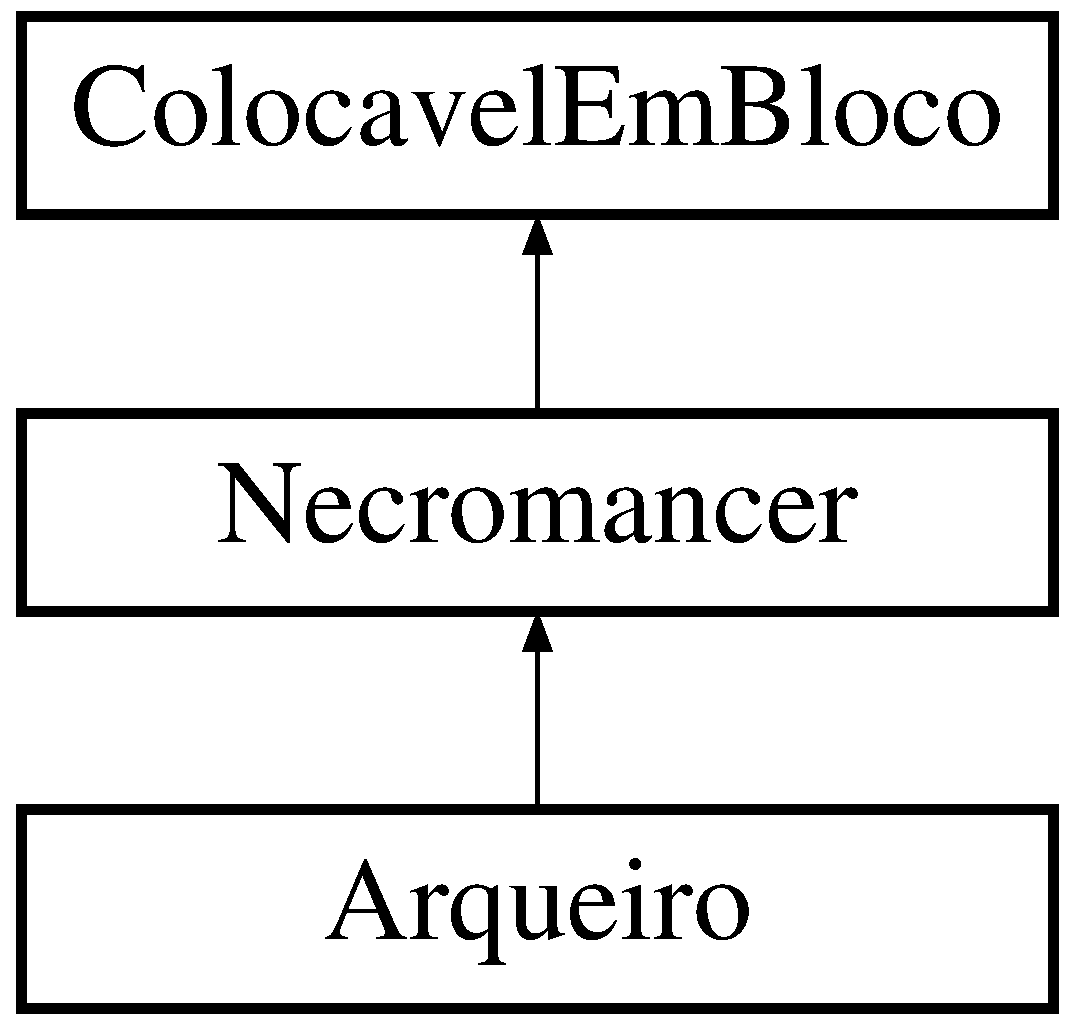
\includegraphics[height=3.000000cm]{class_arqueiro}
\end{center}
\end{figure}
\subsection*{Public Member Functions}
\begin{DoxyCompactItemize}
\item 
\mbox{\Hypertarget{class_arqueiro_a5b2f58461e4f228fc319a1ec872c175d}\label{class_arqueiro_a5b2f58461e4f228fc319a1ec872c175d}} 
\mbox{\hyperlink{class_arqueiro_a5b2f58461e4f228fc319a1ec872c175d}{Arqueiro}} ()
\begin{DoxyCompactList}\small\item\em Construct a new \mbox{\hyperlink{class_arqueiro}{Arqueiro}}\+:\+: \mbox{\hyperlink{class_arqueiro}{Arqueiro}} object. \end{DoxyCompactList}\end{DoxyCompactItemize}
\subsection*{Additional Inherited Members}


\subsection{Detailed Description}


Definition at line 70 of file Necromancer.\+hpp.



The documentation for this class was generated from the following files\+:\begin{DoxyCompactItemize}
\item 
include/\mbox{\hyperlink{_necromancer_8hpp}{Necromancer.\+hpp}}\item 
src/\mbox{\hyperlink{_necromancer_8cpp}{Necromancer.\+cpp}}\end{DoxyCompactItemize}

\hypertarget{class_bloco}{}\section{Bloco Class Reference}
\label{class_bloco}\index{Bloco@{Bloco}}
\subsection*{Public Member Functions}
\begin{DoxyCompactItemize}
\item 
\mbox{\Hypertarget{class_bloco_a920ab5b6599552d1ba6ece51bb132626}\label{class_bloco_a920ab5b6599552d1ba6ece51bb132626}} 
\mbox{\hyperlink{class_bloco_a920ab5b6599552d1ba6ece51bb132626}{Bloco}} ()
\begin{DoxyCompactList}\small\item\em Construct a new \mbox{\hyperlink{class_bloco}{Bloco}}\+:\+: \mbox{\hyperlink{class_bloco}{Bloco}} object. \end{DoxyCompactList}\item 
\mbox{\hyperlink{class_bloco_a1e474398aae75176e9d6bb14b8258541}{Bloco}} (\mbox{\hyperlink{class_colocavel_em_bloco}{Colocavel\+Em\+Bloco}} $\ast$)
\begin{DoxyCompactList}\small\item\em Construct a new \mbox{\hyperlink{class_bloco}{Bloco}}\+:\+: \mbox{\hyperlink{class_bloco}{Bloco}} object. \end{DoxyCompactList}\item 
bool \mbox{\hyperlink{class_bloco_ad5e26f6c5636ac72db653bd1329d5e2e}{preenche}} (\mbox{\hyperlink{class_colocavel_em_bloco}{Colocavel\+Em\+Bloco}} $\ast$)
\item 
bool \mbox{\hyperlink{class_bloco_a8260c149942e04f10f069696a6363451}{limpa}} ()
\end{DoxyCompactItemize}
\subsection*{Public Attributes}
\begin{DoxyCompactItemize}
\item 
\mbox{\Hypertarget{class_bloco_aa453b9d7d8ad875974c09e2c8b21ba73}\label{class_bloco_aa453b9d7d8ad875974c09e2c8b21ba73}} 
bool {\bfseries vazio}
\item 
\mbox{\Hypertarget{class_bloco_a638a917a143c421c404483437004a422}\label{class_bloco_a638a917a143c421c404483437004a422}} 
\mbox{\hyperlink{class_colocavel_em_bloco}{Colocavel\+Em\+Bloco}} $\ast$ {\bfseries conteudo}
\end{DoxyCompactItemize}


\subsection{Detailed Description}


Definition at line 38 of file Bloco.\+hpp.



\subsection{Constructor \& Destructor Documentation}
\mbox{\Hypertarget{class_bloco_a1e474398aae75176e9d6bb14b8258541}\label{class_bloco_a1e474398aae75176e9d6bb14b8258541}} 
\index{Bloco@{Bloco}!Bloco@{Bloco}}
\index{Bloco@{Bloco}!Bloco@{Bloco}}
\subsubsection{\texorpdfstring{Bloco()}{Bloco()}}
{\footnotesize\ttfamily Bloco\+::\+Bloco (\begin{DoxyParamCaption}\item[{\mbox{\hyperlink{class_colocavel_em_bloco}{Colocavel\+Em\+Bloco}} $\ast$}]{conteudo }\end{DoxyParamCaption})}



Construct a new \mbox{\hyperlink{class_bloco}{Bloco}}\+:\+: \mbox{\hyperlink{class_bloco}{Bloco}} object. 


\begin{DoxyParams}{Parameters}
{\em conteudo} & \\
\hline
\end{DoxyParams}


Definition at line 32 of file Bloco.\+cpp.


\begin{DoxyCode}
32                                        \{
33     this->conteudo = conteudo;
34     this->vazio = \textcolor{keyword}{false};
35 \}
\end{DoxyCode}


\subsection{Member Function Documentation}
\mbox{\Hypertarget{class_bloco_a8260c149942e04f10f069696a6363451}\label{class_bloco_a8260c149942e04f10f069696a6363451}} 
\index{Bloco@{Bloco}!limpa@{limpa}}
\index{limpa@{limpa}!Bloco@{Bloco}}
\subsubsection{\texorpdfstring{limpa()}{limpa()}}
{\footnotesize\ttfamily bool Bloco\+::limpa (\begin{DoxyParamCaption}{ }\end{DoxyParamCaption})}

\begin{DoxyReturn}{Returns}
true 

false 
\end{DoxyReturn}


Definition at line 57 of file Bloco.\+cpp.


\begin{DoxyCode}
57                   \{
58     \textcolor{keywordflow}{if} (this->vazio) \textcolor{keywordflow}{return} \textcolor{keyword}{false};
59     this->conteudo = \textcolor{keyword}{nullptr};
60     this->vazio = \textcolor{keyword}{true};
61     \textcolor{keywordflow}{return} \textcolor{keyword}{true};
62 \}
\end{DoxyCode}
\mbox{\Hypertarget{class_bloco_ad5e26f6c5636ac72db653bd1329d5e2e}\label{class_bloco_ad5e26f6c5636ac72db653bd1329d5e2e}} 
\index{Bloco@{Bloco}!preenche@{preenche}}
\index{preenche@{preenche}!Bloco@{Bloco}}
\subsubsection{\texorpdfstring{preenche()}{preenche()}}
{\footnotesize\ttfamily bool Bloco\+::preenche (\begin{DoxyParamCaption}\item[{\mbox{\hyperlink{class_colocavel_em_bloco}{Colocavel\+Em\+Bloco}} $\ast$}]{c }\end{DoxyParamCaption})}


\begin{DoxyParams}{Parameters}
{\em c} & \\
\hline
\end{DoxyParams}
\begin{DoxyReturn}{Returns}
true 

false 
\end{DoxyReturn}


Definition at line 44 of file Bloco.\+cpp.


\begin{DoxyCode}
44                                         \{
45     \textcolor{keywordflow}{if} (!this->vazio) \textcolor{keywordflow}{return} \textcolor{keyword}{false};
46     this->conteudo = c;
47     this->vazio = \textcolor{keyword}{false};
48     \textcolor{keywordflow}{return} \textcolor{keyword}{true};
49 \}
\end{DoxyCode}


The documentation for this class was generated from the following files\+:\begin{DoxyCompactItemize}
\item 
include/\mbox{\hyperlink{_bloco_8hpp}{Bloco.\+hpp}}\item 
src/\mbox{\hyperlink{_bloco_8cpp}{Bloco.\+cpp}}\end{DoxyCompactItemize}

\hypertarget{class_button}{}\section{Button Class Reference}
\label{class_button}\index{Button@{Button}}
\subsection*{Public Member Functions}
\begin{DoxyCompactItemize}
\item 
\mbox{\Hypertarget{class_button_a3b36df1ae23c58aedb9e15a713159459}\label{class_button_a3b36df1ae23c58aedb9e15a713159459}} 
\mbox{\hyperlink{class_button_a3b36df1ae23c58aedb9e15a713159459}{Button}} ()
\begin{DoxyCompactList}\small\item\em Construct a new \mbox{\hyperlink{class_button}{Button}}\+:\+: \mbox{\hyperlink{class_button}{Button}} object. \end{DoxyCompactList}\item 
void \mbox{\hyperlink{class_button_a3abfce268def79881b95d7286a69ec19}{set\+Position\+Size\+Type}} (int x, int y, int width, int height, Button\+Type type)
\item 
void \mbox{\hyperlink{class_button_aa05597e01e195bb5901fc206bc0938a3}{handle\+Event}} (S\+D\+L\+\_\+\+Event $\ast$e, Game $\ast$game)
\item 
void \mbox{\hyperlink{class_button_addeed0141de6e58e0c5f94a4443f7103}{set\+PositionX}} (int x)
\item 
void \mbox{\hyperlink{class_button_a05e92fd7e167df2301247cc022d2694d}{set\+PositionY}} (int y)
\item 
void \mbox{\hyperlink{class_button_a15290e9b24eb7a52a698cc387670aed5}{set\+General\+Button\+Width}} (int width)
\item 
void \mbox{\hyperlink{class_button_aa3b0f5ac8b230e66983a83b6f4c8d440}{set\+General\+Button\+Height}} (int height)
\item 
int \mbox{\hyperlink{class_button_a9bcc23f4a459821144cb0ffdc7c6e338}{get\+PositionX}} ()
\item 
int \mbox{\hyperlink{class_button_a73237a0eeb7ae52d3f5d1c16eb794775}{get\+PositionY}} ()
\item 
int \mbox{\hyperlink{class_button_ac30c0f7242a6514c3b8a0d8b5c1135e6}{get\+General\+Button\+Width}} ()
\item 
int \mbox{\hyperlink{class_button_a577d80e982292d7b17584d11e650dca6}{get\+General\+Button\+Height}} ()
\item 
void \mbox{\hyperlink{class_button_a9d08f75c72f8ba5eddb857cbae0d4c77}{set\+Button\+Type}} (Button\+Type type)
\item 
Button\+Type \mbox{\hyperlink{class_button_afb53df1bb22e22c20d15b055cfa878dc}{get\+Button\+Type}} ()
\end{DoxyCompactItemize}


\subsection{Detailed Description}


Definition at line 48 of file Button.\+hpp.



\subsection{Member Function Documentation}
\mbox{\Hypertarget{class_button_afb53df1bb22e22c20d15b055cfa878dc}\label{class_button_afb53df1bb22e22c20d15b055cfa878dc}} 
\index{Button@{Button}!get\+Button\+Type@{get\+Button\+Type}}
\index{get\+Button\+Type@{get\+Button\+Type}!Button@{Button}}
\subsubsection{\texorpdfstring{get\+Button\+Type()}{getButtonType()}}
{\footnotesize\ttfamily Button\+Type Button\+::get\+Button\+Type (\begin{DoxyParamCaption}{ }\end{DoxyParamCaption})}

\begin{DoxyReturn}{Returns}
Button\+Type 
\end{DoxyReturn}


Definition at line 175 of file Button.\+cpp.


\begin{DoxyCode}
175                                  \{
176     \textcolor{keywordflow}{return} buttonType;
177 \}
\end{DoxyCode}
\mbox{\Hypertarget{class_button_a577d80e982292d7b17584d11e650dca6}\label{class_button_a577d80e982292d7b17584d11e650dca6}} 
\index{Button@{Button}!get\+General\+Button\+Height@{get\+General\+Button\+Height}}
\index{get\+General\+Button\+Height@{get\+General\+Button\+Height}!Button@{Button}}
\subsubsection{\texorpdfstring{get\+General\+Button\+Height()}{getGeneralButtonHeight()}}
{\footnotesize\ttfamily int Button\+::get\+General\+Button\+Height (\begin{DoxyParamCaption}{ }\end{DoxyParamCaption})}

\begin{DoxyReturn}{Returns}
int 
\end{DoxyReturn}


Definition at line 157 of file Button.\+cpp.


\begin{DoxyCode}
157                                    \{
158     \textcolor{keywordflow}{return} button\_height;
159 \}
\end{DoxyCode}
\mbox{\Hypertarget{class_button_ac30c0f7242a6514c3b8a0d8b5c1135e6}\label{class_button_ac30c0f7242a6514c3b8a0d8b5c1135e6}} 
\index{Button@{Button}!get\+General\+Button\+Width@{get\+General\+Button\+Width}}
\index{get\+General\+Button\+Width@{get\+General\+Button\+Width}!Button@{Button}}
\subsubsection{\texorpdfstring{get\+General\+Button\+Width()}{getGeneralButtonWidth()}}
{\footnotesize\ttfamily int Button\+::get\+General\+Button\+Width (\begin{DoxyParamCaption}{ }\end{DoxyParamCaption})}

\begin{DoxyReturn}{Returns}
int 
\end{DoxyReturn}


Definition at line 148 of file Button.\+cpp.


\begin{DoxyCode}
148                                   \{
149     \textcolor{keywordflow}{return} button\_width;
150 \}
\end{DoxyCode}
\mbox{\Hypertarget{class_button_a9bcc23f4a459821144cb0ffdc7c6e338}\label{class_button_a9bcc23f4a459821144cb0ffdc7c6e338}} 
\index{Button@{Button}!get\+PositionX@{get\+PositionX}}
\index{get\+PositionX@{get\+PositionX}!Button@{Button}}
\subsubsection{\texorpdfstring{get\+Position\+X()}{getPositionX()}}
{\footnotesize\ttfamily int Button\+::get\+PositionX (\begin{DoxyParamCaption}{ }\end{DoxyParamCaption})}

\begin{DoxyReturn}{Returns}
int 
\end{DoxyReturn}


Definition at line 130 of file Button.\+cpp.


\begin{DoxyCode}
130                          \{
131     \textcolor{keywordflow}{return} position\_x;
132 \}
\end{DoxyCode}
\mbox{\Hypertarget{class_button_a73237a0eeb7ae52d3f5d1c16eb794775}\label{class_button_a73237a0eeb7ae52d3f5d1c16eb794775}} 
\index{Button@{Button}!get\+PositionY@{get\+PositionY}}
\index{get\+PositionY@{get\+PositionY}!Button@{Button}}
\subsubsection{\texorpdfstring{get\+Position\+Y()}{getPositionY()}}
{\footnotesize\ttfamily int Button\+::get\+PositionY (\begin{DoxyParamCaption}{ }\end{DoxyParamCaption})}

\begin{DoxyReturn}{Returns}
int 
\end{DoxyReturn}


Definition at line 139 of file Button.\+cpp.


\begin{DoxyCode}
139                          \{
140     \textcolor{keywordflow}{return} position\_y;
141 \}
\end{DoxyCode}
\mbox{\Hypertarget{class_button_aa05597e01e195bb5901fc206bc0938a3}\label{class_button_aa05597e01e195bb5901fc206bc0938a3}} 
\index{Button@{Button}!handle\+Event@{handle\+Event}}
\index{handle\+Event@{handle\+Event}!Button@{Button}}
\subsubsection{\texorpdfstring{handle\+Event()}{handleEvent()}}
{\footnotesize\ttfamily void Button\+::handle\+Event (\begin{DoxyParamCaption}\item[{S\+D\+L\+\_\+\+Event $\ast$}]{e,  }\item[{Game $\ast$}]{game }\end{DoxyParamCaption})}


\begin{DoxyParams}{Parameters}
{\em e} & \\
\hline
{\em game} & \\
\hline
\end{DoxyParams}


Definition at line 51 of file Button.\+cpp.


\begin{DoxyCode}
51                                                   \{
52     \textcolor{keywordflow}{if} (e->type == SDL\_MOUSEBUTTONDOWN) \{
53         \textcolor{comment}{// Get mouse position}
54         \textcolor{keywordtype}{int} x, y;
55         SDL\_GetMouseState(&x, &y);
56         \textcolor{comment}{// Check if mouse is in Button}
57         \textcolor{keywordtype}{bool} inside = \textcolor{keyword}{false};
58         \textcolor{keywordflow}{if} (y > position\_y && y < (position\_y + button\_height)) \{
59             \textcolor{keywordflow}{if} (x > position\_x && x < (position\_x + button\_width)) \{
60                 inside = \textcolor{keyword}{true};
61             \}
62         \}
63 
64         \textcolor{keywordflow}{if} (inside) \{
65             \textcolor{keywordflow}{switch} (e->type) \{
66                 \textcolor{keywordflow}{case} SDL\_MOUSEBUTTONDOWN:
67                     \textcolor{keywordflow}{switch} (buttonType) \{
68                     \textcolor{keywordflow}{case} BUTTON\_PLAY:
69                         game->setGameRunning(GAME\_PLAY);
70                         \textcolor{keywordflow}{break};
71                     \textcolor{keywordflow}{case} BUTTON\_CREDITS:
72                         game->setGameRunning(GAME\_CREDITS);
73                         \textcolor{keywordflow}{break};
74                     \textcolor{keywordflow}{case} BUTTON\_QUIT:
75                         game->setGameRunning(GAME\_QUIT);
76                         \textcolor{keywordflow}{break};
77                     \textcolor{keywordflow}{case} BUTTON\_BACK\_CREDITS:
78                         game->setGameRunning(GAME\_MENU);
79                         \textcolor{keywordflow}{break};
80                     \textcolor{keywordflow}{case} BUTTON\_BACK\_GAME:
81                         game->setGameRunning(GAME\_PLAY);
82                     \}
83                 \textcolor{keywordflow}{break};
84             \}
85         \}
86     \}
87 \}
\end{DoxyCode}
\mbox{\Hypertarget{class_button_a9d08f75c72f8ba5eddb857cbae0d4c77}\label{class_button_a9d08f75c72f8ba5eddb857cbae0d4c77}} 
\index{Button@{Button}!set\+Button\+Type@{set\+Button\+Type}}
\index{set\+Button\+Type@{set\+Button\+Type}!Button@{Button}}
\subsubsection{\texorpdfstring{set\+Button\+Type()}{setButtonType()}}
{\footnotesize\ttfamily void Button\+::set\+Button\+Type (\begin{DoxyParamCaption}\item[{Button\+Type}]{type }\end{DoxyParamCaption})}


\begin{DoxyParams}{Parameters}
{\em type} & \\
\hline
\end{DoxyParams}


Definition at line 166 of file Button.\+cpp.


\begin{DoxyCode}
166                                           \{
167     buttonType = type;
168 \}
\end{DoxyCode}
\mbox{\Hypertarget{class_button_aa3b0f5ac8b230e66983a83b6f4c8d440}\label{class_button_aa3b0f5ac8b230e66983a83b6f4c8d440}} 
\index{Button@{Button}!set\+General\+Button\+Height@{set\+General\+Button\+Height}}
\index{set\+General\+Button\+Height@{set\+General\+Button\+Height}!Button@{Button}}
\subsubsection{\texorpdfstring{set\+General\+Button\+Height()}{setGeneralButtonHeight()}}
{\footnotesize\ttfamily void Button\+::set\+General\+Button\+Height (\begin{DoxyParamCaption}\item[{int}]{height }\end{DoxyParamCaption})}


\begin{DoxyParams}{Parameters}
{\em height} & \\
\hline
\end{DoxyParams}


Definition at line 121 of file Button.\+cpp.


\begin{DoxyCode}
121                                               \{
122     button\_height = height;
123 \}
\end{DoxyCode}
\mbox{\Hypertarget{class_button_a15290e9b24eb7a52a698cc387670aed5}\label{class_button_a15290e9b24eb7a52a698cc387670aed5}} 
\index{Button@{Button}!set\+General\+Button\+Width@{set\+General\+Button\+Width}}
\index{set\+General\+Button\+Width@{set\+General\+Button\+Width}!Button@{Button}}
\subsubsection{\texorpdfstring{set\+General\+Button\+Width()}{setGeneralButtonWidth()}}
{\footnotesize\ttfamily void Button\+::set\+General\+Button\+Width (\begin{DoxyParamCaption}\item[{int}]{width }\end{DoxyParamCaption})}


\begin{DoxyParams}{Parameters}
{\em width} & \\
\hline
\end{DoxyParams}


Definition at line 112 of file Button.\+cpp.


\begin{DoxyCode}
112                                             \{
113     button\_width = width;
114 \}
\end{DoxyCode}
\mbox{\Hypertarget{class_button_a3abfce268def79881b95d7286a69ec19}\label{class_button_a3abfce268def79881b95d7286a69ec19}} 
\index{Button@{Button}!set\+Position\+Size\+Type@{set\+Position\+Size\+Type}}
\index{set\+Position\+Size\+Type@{set\+Position\+Size\+Type}!Button@{Button}}
\subsubsection{\texorpdfstring{set\+Position\+Size\+Type()}{setPositionSizeType()}}
{\footnotesize\ttfamily void Button\+::set\+Position\+Size\+Type (\begin{DoxyParamCaption}\item[{int}]{x,  }\item[{int}]{y,  }\item[{int}]{width,  }\item[{int}]{height,  }\item[{Button\+Type}]{type }\end{DoxyParamCaption})}


\begin{DoxyParams}{Parameters}
{\em x} & \\
\hline
{\em y} & \\
\hline
{\em width} & \\
\hline
{\em height} & \\
\hline
{\em type} & \\
\hline
\end{DoxyParams}


Definition at line 37 of file Button.\+cpp.


\begin{DoxyCode}
37                                                                                      \{
38     position\_x = x;
39     position\_y = y;
40     button\_width = width;
41     button\_height = height;
42     buttonType = type;
43 \}
\end{DoxyCode}
\mbox{\Hypertarget{class_button_addeed0141de6e58e0c5f94a4443f7103}\label{class_button_addeed0141de6e58e0c5f94a4443f7103}} 
\index{Button@{Button}!set\+PositionX@{set\+PositionX}}
\index{set\+PositionX@{set\+PositionX}!Button@{Button}}
\subsubsection{\texorpdfstring{set\+Position\+X()}{setPositionX()}}
{\footnotesize\ttfamily void Button\+::set\+PositionX (\begin{DoxyParamCaption}\item[{int}]{x }\end{DoxyParamCaption})}


\begin{DoxyParams}{Parameters}
{\em x} & \\
\hline
\end{DoxyParams}


Definition at line 94 of file Button.\+cpp.


\begin{DoxyCode}
94                                \{
95     position\_x = x;
96 \}
\end{DoxyCode}
\mbox{\Hypertarget{class_button_a05e92fd7e167df2301247cc022d2694d}\label{class_button_a05e92fd7e167df2301247cc022d2694d}} 
\index{Button@{Button}!set\+PositionY@{set\+PositionY}}
\index{set\+PositionY@{set\+PositionY}!Button@{Button}}
\subsubsection{\texorpdfstring{set\+Position\+Y()}{setPositionY()}}
{\footnotesize\ttfamily void Button\+::set\+PositionY (\begin{DoxyParamCaption}\item[{int}]{y }\end{DoxyParamCaption})}


\begin{DoxyParams}{Parameters}
{\em y} & \\
\hline
\end{DoxyParams}


Definition at line 103 of file Button.\+cpp.


\begin{DoxyCode}
103                                \{
104     position\_y = y;
105 \}
\end{DoxyCode}


The documentation for this class was generated from the following files\+:\begin{DoxyCompactItemize}
\item 
include/\mbox{\hyperlink{_button_8hpp}{Button.\+hpp}}\item 
src/\mbox{\hyperlink{_button_8cpp}{Button.\+cpp}}\end{DoxyCompactItemize}

\hypertarget{class_cavaleiro}{}\section{Cavaleiro Class Reference}
\label{class_cavaleiro}\index{Cavaleiro@{Cavaleiro}}
Inheritance diagram for Cavaleiro\+:\begin{figure}[H]
\begin{center}
\leavevmode
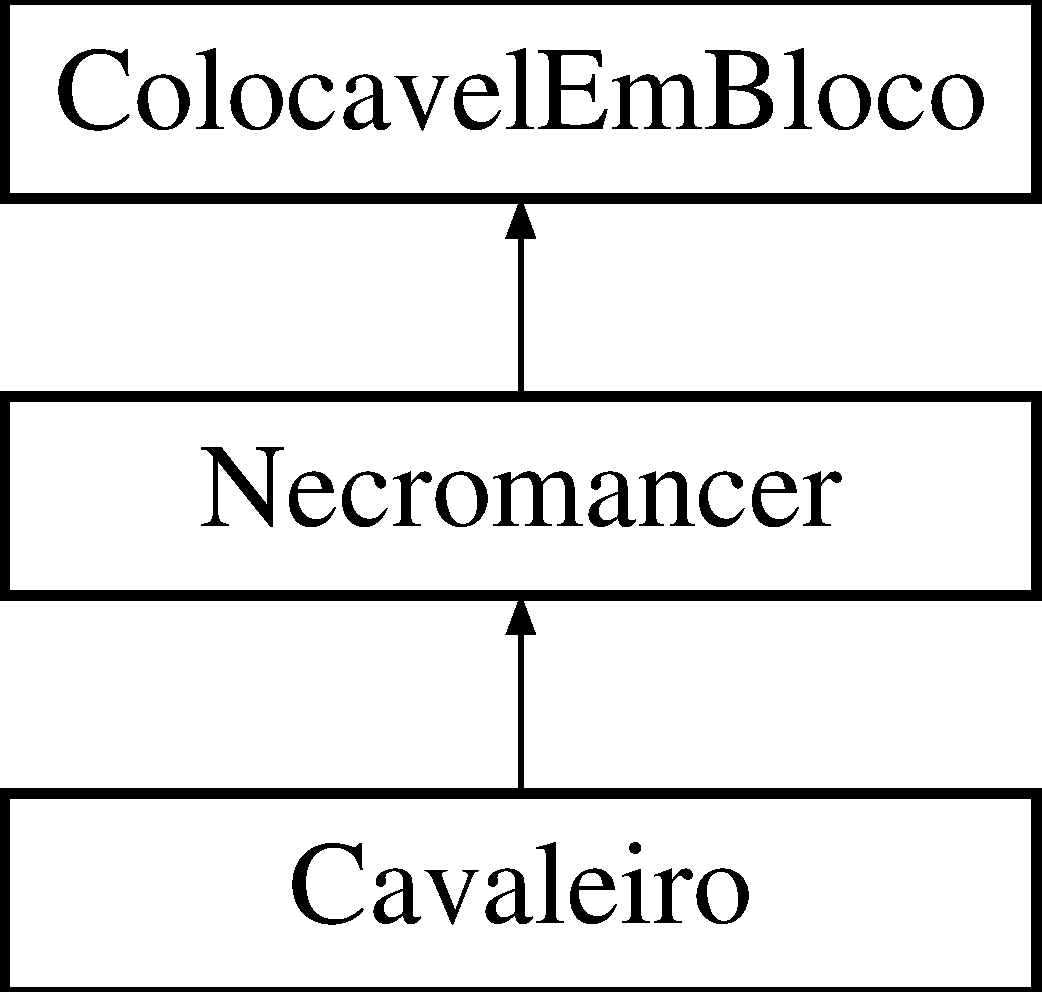
\includegraphics[height=3.000000cm]{class_cavaleiro}
\end{center}
\end{figure}
\subsection*{Public Member Functions}
\begin{DoxyCompactItemize}
\item 
\mbox{\Hypertarget{class_cavaleiro_a3941e46c628ff9fb3c27e73936795df7}\label{class_cavaleiro_a3941e46c628ff9fb3c27e73936795df7}} 
\mbox{\hyperlink{class_cavaleiro_a3941e46c628ff9fb3c27e73936795df7}{Cavaleiro}} ()
\begin{DoxyCompactList}\small\item\em Construct a new \mbox{\hyperlink{class_cavaleiro}{Cavaleiro}}\+:\+: \mbox{\hyperlink{class_cavaleiro}{Cavaleiro}} object. \end{DoxyCompactList}\end{DoxyCompactItemize}
\subsection*{Additional Inherited Members}


\subsection{Detailed Description}


Definition at line 63 of file Necromancer.\+hpp.



The documentation for this class was generated from the following files\+:\begin{DoxyCompactItemize}
\item 
include/\mbox{\hyperlink{_necromancer_8hpp}{Necromancer.\+hpp}}\item 
src/\mbox{\hyperlink{_necromancer_8cpp}{Necromancer.\+cpp}}\end{DoxyCompactItemize}

\hypertarget{class_colocavel_em_bloco}{}\section{Colocavel\+Em\+Bloco Class Reference}
\label{class_colocavel_em_bloco}\index{Colocavel\+Em\+Bloco@{Colocavel\+Em\+Bloco}}
Inheritance diagram for Colocavel\+Em\+Bloco\+:\begin{figure}[H]
\begin{center}
\leavevmode
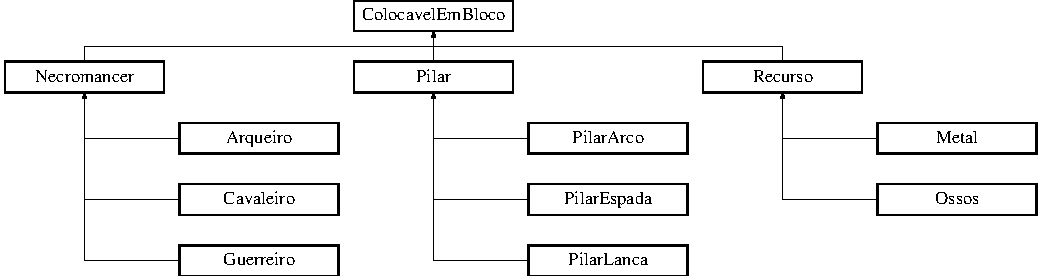
\includegraphics[height=3.703704cm]{class_colocavel_em_bloco}
\end{center}
\end{figure}
\subsection*{Public Member Functions}
\begin{DoxyCompactItemize}
\item 
\mbox{\Hypertarget{class_colocavel_em_bloco_a3e99f0924333aa4473cc59588acec5dc}\label{class_colocavel_em_bloco_a3e99f0924333aa4473cc59588acec5dc}} 
\mbox{\hyperlink{class_colocavel_em_bloco_a3e99f0924333aa4473cc59588acec5dc}{Colocavel\+Em\+Bloco}} ()
\begin{DoxyCompactList}\small\item\em Construct a new Colocavel Em \mbox{\hyperlink{class_bloco}{Bloco}}\+:\+: Colocavel Em \mbox{\hyperlink{class_bloco}{Bloco}} object. \end{DoxyCompactList}\item 
bool \mbox{\hyperlink{class_colocavel_em_bloco_a89177aadb9f7fd73431adcb29b90f887}{mata}} ()
\item 
bool \mbox{\hyperlink{class_colocavel_em_bloco_a82f12304bcb919f4fe3fc765d00a3d0f}{revive}} ()
\item 
void \mbox{\hyperlink{class_colocavel_em_bloco_a1d45029183e2b8fe4790d44ca0fa3484}{set\+Ativo}} (bool a)
\end{DoxyCompactItemize}
\subsection*{Public Attributes}
\begin{DoxyCompactItemize}
\item 
\mbox{\Hypertarget{class_colocavel_em_bloco_a8c5d017d88f31ff3d8e5dfb01ac92d76}\label{class_colocavel_em_bloco_a8c5d017d88f31ff3d8e5dfb01ac92d76}} 
bool {\bfseries vivo}
\item 
\mbox{\Hypertarget{class_colocavel_em_bloco_ae0ab0d922be3835d8fa523a8b16769bf}\label{class_colocavel_em_bloco_ae0ab0d922be3835d8fa523a8b16769bf}} 
unsigned short {\bfseries x}
\item 
\mbox{\Hypertarget{class_colocavel_em_bloco_ac43768b1cb415acedb4edd9c678f7895}\label{class_colocavel_em_bloco_ac43768b1cb415acedb4edd9c678f7895}} 
unsigned short {\bfseries y}
\item 
\mbox{\Hypertarget{class_colocavel_em_bloco_af766227d1bcfb9858a0d80a623bcc283}\label{class_colocavel_em_bloco_af766227d1bcfb9858a0d80a623bcc283}} 
unsigned short {\bfseries time}
\item 
\mbox{\Hypertarget{class_colocavel_em_bloco_a988a57fa9f64a350685d6e9d05cf2643}\label{class_colocavel_em_bloco_a988a57fa9f64a350685d6e9d05cf2643}} 
Tipo\+Conteudo\+Bloco {\bfseries tipo}
\item 
\mbox{\Hypertarget{class_colocavel_em_bloco_a5b6576486062c11fce316071d1535137}\label{class_colocavel_em_bloco_a5b6576486062c11fce316071d1535137}} 
bool {\bfseries ativo}
\end{DoxyCompactItemize}


\subsection{Detailed Description}


Definition at line 26 of file Bloco.\+hpp.



\subsection{Member Function Documentation}
\mbox{\Hypertarget{class_colocavel_em_bloco_a89177aadb9f7fd73431adcb29b90f887}\label{class_colocavel_em_bloco_a89177aadb9f7fd73431adcb29b90f887}} 
\index{Colocavel\+Em\+Bloco@{Colocavel\+Em\+Bloco}!mata@{mata}}
\index{mata@{mata}!Colocavel\+Em\+Bloco@{Colocavel\+Em\+Bloco}}
\subsubsection{\texorpdfstring{mata()}{mata()}}
{\footnotesize\ttfamily bool Colocavel\+Em\+Bloco\+::mata (\begin{DoxyParamCaption}{ }\end{DoxyParamCaption})}

\begin{DoxyReturn}{Returns}
true 

false 
\end{DoxyReturn}


Definition at line 87 of file Bloco.\+cpp.



Referenced by Player\+::\+Player().


\begin{DoxyCode}
87                             \{
88     \textcolor{keywordflow}{if} (this->vivo) \{
89         this->vivo = \textcolor{keyword}{false};
90         this->x = -1;
91         this->y = -1;
92         \textcolor{keywordflow}{return} \textcolor{keyword}{true};
93     \}
94     \textcolor{keywordflow}{return} \textcolor{keyword}{false};
95 \}
\end{DoxyCode}
\mbox{\Hypertarget{class_colocavel_em_bloco_a82f12304bcb919f4fe3fc765d00a3d0f}\label{class_colocavel_em_bloco_a82f12304bcb919f4fe3fc765d00a3d0f}} 
\index{Colocavel\+Em\+Bloco@{Colocavel\+Em\+Bloco}!revive@{revive}}
\index{revive@{revive}!Colocavel\+Em\+Bloco@{Colocavel\+Em\+Bloco}}
\subsubsection{\texorpdfstring{revive()}{revive()}}
{\footnotesize\ttfamily bool Colocavel\+Em\+Bloco\+::revive (\begin{DoxyParamCaption}{ }\end{DoxyParamCaption})}

\begin{DoxyReturn}{Returns}
true 

false 
\end{DoxyReturn}


Definition at line 103 of file Bloco.\+cpp.


\begin{DoxyCode}
103                               \{
104     \textcolor{keywordflow}{if} (this->vivo)
105         \textcolor{keywordflow}{return} \textcolor{keyword}{false};
106 
107     this->vivo = \textcolor{keyword}{true};
108     \textcolor{keywordflow}{return} \textcolor{keyword}{true};
109 \}
\end{DoxyCode}
\mbox{\Hypertarget{class_colocavel_em_bloco_a1d45029183e2b8fe4790d44ca0fa3484}\label{class_colocavel_em_bloco_a1d45029183e2b8fe4790d44ca0fa3484}} 
\index{Colocavel\+Em\+Bloco@{Colocavel\+Em\+Bloco}!set\+Ativo@{set\+Ativo}}
\index{set\+Ativo@{set\+Ativo}!Colocavel\+Em\+Bloco@{Colocavel\+Em\+Bloco}}
\subsubsection{\texorpdfstring{set\+Ativo()}{setAtivo()}}
{\footnotesize\ttfamily void Colocavel\+Em\+Bloco\+::set\+Ativo (\begin{DoxyParamCaption}\item[{bool}]{a }\end{DoxyParamCaption})}


\begin{DoxyParams}{Parameters}
{\em a} & \\
\hline
\end{DoxyParams}


Definition at line 77 of file Bloco.\+cpp.



Referenced by Controlador\+::novo\+\_\+jogo().


\begin{DoxyCode}
77                                       \{
78     ativo = a;
79 \}
\end{DoxyCode}


The documentation for this class was generated from the following files\+:\begin{DoxyCompactItemize}
\item 
include/\mbox{\hyperlink{_bloco_8hpp}{Bloco.\+hpp}}\item 
src/\mbox{\hyperlink{_bloco_8cpp}{Bloco.\+cpp}}\end{DoxyCompactItemize}

\hypertarget{class_controlador}{}\section{Controlador Class Reference}
\label{class_controlador}\index{Controlador@{Controlador}}
\subsection*{Public Member Functions}
\begin{DoxyCompactItemize}
\item 
\mbox{\Hypertarget{class_controlador_a17db08229680461d4d1a2110a92ccf78}\label{class_controlador_a17db08229680461d4d1a2110a92ccf78}} 
\mbox{\hyperlink{class_controlador_a17db08229680461d4d1a2110a92ccf78}{Controlador}} ()
\begin{DoxyCompactList}\small\item\em Construct a new \mbox{\hyperlink{class_controlador}{Controlador}}\+:\+: \mbox{\hyperlink{class_controlador}{Controlador}} object. \end{DoxyCompactList}\item 
bool \mbox{\hyperlink{class_controlador_a89652e27b5fc06fa0489e6bae0328d33}{novo\+\_\+jogo}} (bool, bool)
\item 
\mbox{\Hypertarget{class_controlador_ab1464581160e7baba397b32ac41315ab}\label{class_controlador_ab1464581160e7baba397b32ac41315ab}} 
bool {\bfseries salvar\+\_\+jogo} (std\+::string path)
\item 
\mbox{\Hypertarget{class_controlador_a6fac98d6cc32e0f413d55755000fca3a}\label{class_controlador_a6fac98d6cc32e0f413d55755000fca3a}} 
bool {\bfseries carregar\+\_\+jogo} (std\+::string path)
\item 
bool \mbox{\hyperlink{class_controlador_a5c4aa9d015704147f6b24ca9a90c94c1}{criar\+\_\+pilar}} (\mbox{\hyperlink{class_player}{Player}} $\ast$, Tipo\+Pilar, unsigned short, unsigned short)
\item 
bool \mbox{\hyperlink{class_controlador_a7c0445d2f378ff7d9b26d2cc77059484}{fortalecer\+\_\+pilar}} (\mbox{\hyperlink{class_player}{Player}} $\ast$, Tipo\+Pilar)
\item 
bool \mbox{\hyperlink{class_controlador_aa444d0b080f4d4ecc397819d97098a3a}{criar\+\_\+necromancer}} (\mbox{\hyperlink{class_player}{Player}} $\ast$, Tipo\+Necromancer, unsigned short, unsigned short)
\item 
bool \mbox{\hyperlink{class_controlador_a417c5d209a4fb165ecc03063b3adef80}{fortalecer\+\_\+necromancer}} (\mbox{\hyperlink{class_player}{Player}} $\ast$, Tipo\+Necromancer)
\item 
bool \mbox{\hyperlink{class_controlador_a2455948558b79285060dbd2dd8d15bf1}{matar}} (unsigned short, unsigned short)
\item 
bool \mbox{\hyperlink{class_controlador_a75328c4987fa242b36531edac623ff3e}{pode\+\_\+movimentar}} (\mbox{\hyperlink{class_player}{Player}} $\ast$, unsigned short, unsigned short, unsigned short, unsigned short)
\item 
bool \mbox{\hyperlink{class_controlador_a928e6fc0f6cad97f68b4536a802f82bc}{movimentar}} (\mbox{\hyperlink{class_player}{Player}} $\ast$, unsigned short, unsigned short, unsigned short, unsigned short)
\item 
\mbox{\Hypertarget{class_controlador_aa91bbe914a404ef60a4cdef6cf7af4e6}\label{class_controlador_aa91bbe914a404ef60a4cdef6cf7af4e6}} 
void {\bfseries processa\+\_\+jogada} ()
\item 
bool \mbox{\hyperlink{class_controlador_ad7e1f4e5dc199d9499cf1896c3f4fdf1}{alguem\+\_\+ganhou}} ()
\item 
\mbox{\Hypertarget{class_controlador_a55cb7c5d39b6218e62e61fe6a70b6ae3}\label{class_controlador_a55cb7c5d39b6218e62e61fe6a70b6ae3}} 
void {\bfseries muda\+\_\+vez} ()
\item 
void \mbox{\hyperlink{class_controlador_ad836b4790965ddd4b654a42235b8267e}{verifica\+\_\+combate}} (unsigned short, unsigned short)
\item 
void \mbox{\hyperlink{class_controlador_a3f130df13f0c24605a3e34c3edbd2959}{realiza\+\_\+combate}} (unsigned short, unsigned short, unsigned short, unsigned short)
\item 
bool \mbox{\hyperlink{class_controlador_a331d668f08fc4946d79d3742978ef481}{gerou\+\_\+combate}} (unsigned short, unsigned short, unsigned short)
\item 
\mbox{\Hypertarget{class_controlador_a31986f0934c1b40dce19ef1bfbba5cbc}\label{class_controlador_a31986f0934c1b40dce19ef1bfbba5cbc}} 
void {\bfseries print\+\_\+recursos} ()
\item 
\mbox{\Hypertarget{class_controlador_a9190ea722291cb46b8f30024c1cd10af}\label{class_controlador_a9190ea722291cb46b8f30024c1cd10af}} 
void {\bfseries print\+\_\+mapa} ()
\end{DoxyCompactItemize}
\subsection*{Public Attributes}
\begin{DoxyCompactItemize}
\item 
\mbox{\Hypertarget{class_controlador_a8fb90e5dbcda7ce8e855d8c9246df8a7}\label{class_controlador_a8fb90e5dbcda7ce8e855d8c9246df8a7}} 
\mbox{\hyperlink{class_mapa}{Mapa}} {\bfseries mapa}
\item 
\mbox{\Hypertarget{class_controlador_a1e8a704be3d0a15c095c2897e623728d}\label{class_controlador_a1e8a704be3d0a15c095c2897e623728d}} 
\mbox{\hyperlink{class_player}{Player}} {\bfseries jogador}
\item 
\mbox{\Hypertarget{class_controlador_aec1c1cbe4488e23d4b423bf1ba054fd1}\label{class_controlador_aec1c1cbe4488e23d4b423bf1ba054fd1}} 
\mbox{\hyperlink{class_player}{Player}} {\bfseries computador}
\item 
\mbox{\Hypertarget{class_controlador_a34a8141b30a4f090f26eaf656b2b826a}\label{class_controlador_a34a8141b30a4f090f26eaf656b2b826a}} 
Posicao {\bfseries cursor}
\item 
\mbox{\Hypertarget{class_controlador_aad6167445edd710d31143f304a83b900}\label{class_controlador_aad6167445edd710d31143f304a83b900}} 
std\+::list$<$ \mbox{\hyperlink{class_recurso}{Recurso}} $>$ {\bfseries recursos}
\item 
\mbox{\Hypertarget{class_controlador_aceb7b0dfc54dc4bc40d8c6c2fc9a7d0d}\label{class_controlador_aceb7b0dfc54dc4bc40d8c6c2fc9a7d0d}} 
bool {\bfseries jogo\+\_\+terminou}
\item 
\mbox{\Hypertarget{class_controlador_a5b9ba3da648ca06e50066247555af03d}\label{class_controlador_a5b9ba3da648ca06e50066247555af03d}} 
int {\bfseries ganhou}
\item 
\mbox{\Hypertarget{class_controlador_aa50f9470bc51c7f6a9c523f5df9ae320}\label{class_controlador_aa50f9470bc51c7f6a9c523f5df9ae320}} 
bool {\bfseries computador\+\_\+joga}
\item 
\mbox{\Hypertarget{class_controlador_a711a5579c3618d904609a478afca5a78}\label{class_controlador_a711a5579c3618d904609a478afca5a78}} 
unsigned short {\bfseries vez}
\item 
\mbox{\Hypertarget{class_controlador_a1361a922b61a78ff56f97c3d1a2f6830}\label{class_controlador_a1361a922b61a78ff56f97c3d1a2f6830}} 
int {\bfseries vezes}
\end{DoxyCompactItemize}


\subsection{Detailed Description}


Definition at line 26 of file Controlador.\+hpp.



\subsection{Member Function Documentation}
\mbox{\Hypertarget{class_controlador_ad7e1f4e5dc199d9499cf1896c3f4fdf1}\label{class_controlador_ad7e1f4e5dc199d9499cf1896c3f4fdf1}} 
\index{Controlador@{Controlador}!alguem\+\_\+ganhou@{alguem\+\_\+ganhou}}
\index{alguem\+\_\+ganhou@{alguem\+\_\+ganhou}!Controlador@{Controlador}}
\subsubsection{\texorpdfstring{alguem\+\_\+ganhou()}{alguem\_ganhou()}}
{\footnotesize\ttfamily bool Controlador\+::alguem\+\_\+ganhou (\begin{DoxyParamCaption}{ }\end{DoxyParamCaption})}

\begin{DoxyReturn}{Returns}
true 

false 
\end{DoxyReturn}


Definition at line 332 of file Controlador.\+cpp.



References Player\+::perdeu\+\_\+jogo(), and Player\+::pontuacao().


\begin{DoxyCode}
332                                 \{
333     \textcolor{keywordflow}{if} (this->recursos.size() == 0) \{
334         \textcolor{keywordflow}{if} (this->jogador.\mbox{\hyperlink{class_player_a945277689283bc50bd3afef306bf9740}{pontuacao}}() > this->computador.\mbox{\hyperlink{class_player_a945277689283bc50bd3afef306bf9740}{pontuacao}}()) \{
335             this->jogo\_terminou = \textcolor{keyword}{true};
336             this->ganhou = 0;
337             \textcolor{keywordflow}{return} \textcolor{keyword}{true};
338         \}
339         \textcolor{keywordflow}{if} (this->jogador.\mbox{\hyperlink{class_player_a945277689283bc50bd3afef306bf9740}{pontuacao}}() < this->computador.\mbox{\hyperlink{class_player_a945277689283bc50bd3afef306bf9740}{pontuacao}}()) \{
340             this->jogo\_terminou = \textcolor{keyword}{true};
341             this->ganhou = 1;
342             \textcolor{keywordflow}{return} \textcolor{keyword}{true};
343         \}
344 
345         this->jogo\_terminou = \textcolor{keyword}{true};
346         this->ganhou = -1;
347         \textcolor{keywordflow}{return} \textcolor{keyword}{true};
348     \}
349 
350     \textcolor{keywordflow}{if} (this->jogador.\mbox{\hyperlink{class_player_aad208bab9f9f88af5ac34ebe7c31dc61}{perdeu\_jogo}}()) \{
351         this->jogo\_terminou = \textcolor{keyword}{true};
352         this->ganhou = 1;
353         \textcolor{keywordflow}{return} \textcolor{keyword}{true};
354     \}
355     \textcolor{keywordflow}{if} (this->computador.\mbox{\hyperlink{class_player_aad208bab9f9f88af5ac34ebe7c31dc61}{perdeu\_jogo}}()) \{
356         this->jogo\_terminou = \textcolor{keyword}{true};
357         this->ganhou = 0;
358         \textcolor{keywordflow}{return} \textcolor{keyword}{true};
359     \}
360 
361     \textcolor{keywordflow}{return} \textcolor{keyword}{false};
362 \}
\end{DoxyCode}
\mbox{\Hypertarget{class_controlador_aa444d0b080f4d4ecc397819d97098a3a}\label{class_controlador_aa444d0b080f4d4ecc397819d97098a3a}} 
\index{Controlador@{Controlador}!criar\+\_\+necromancer@{criar\+\_\+necromancer}}
\index{criar\+\_\+necromancer@{criar\+\_\+necromancer}!Controlador@{Controlador}}
\subsubsection{\texorpdfstring{criar\+\_\+necromancer()}{criar\_necromancer()}}
{\footnotesize\ttfamily bool Controlador\+::criar\+\_\+necromancer (\begin{DoxyParamCaption}\item[{\mbox{\hyperlink{class_player}{Player}} $\ast$}]{jog,  }\item[{Tipo\+Necromancer}]{nec,  }\item[{unsigned short}]{x,  }\item[{unsigned short}]{y }\end{DoxyParamCaption})}


\begin{DoxyParams}{Parameters}
{\em jog} & \\
\hline
{\em nec} & \\
\hline
{\em x} & \\
\hline
{\em y} & \\
\hline
\end{DoxyParams}
\begin{DoxyReturn}{Returns}
true 

false 
\end{DoxyReturn}


Definition at line 113 of file Controlador.\+cpp.



References Player\+::criar\+\_\+necromancer(), Mapa\+::inserir(), Player\+::necromancer(), and Mapa\+::vazio().


\begin{DoxyCode}
113                                                                                                         \{
114     \textcolor{keywordflow}{if} (jog->\mbox{\hyperlink{class_player_a560ffc698994e73527433dd2bf4d2c0d}{necromancer}}(nec)->vivo) \textcolor{keywordflow}{return} \textcolor{keyword}{false};
115     \textcolor{keywordflow}{if} (!this->mapa.\mbox{\hyperlink{class_mapa_a5bdde997d3c97c5b6fb7d37c124cdf93}{vazio}}(x, y)) \textcolor{keywordflow}{return} \textcolor{keyword}{false};
116     \textcolor{keywordflow}{if} (!jog->\mbox{\hyperlink{class_player_a118c76695a9c1f362a5371381bfe5be3}{criar\_necromancer}}(nec)) \textcolor{keywordflow}{return} \textcolor{keyword}{false};
117 
118     this->mapa.\mbox{\hyperlink{class_mapa_a4dbab5cd3008b39687d8d2edb0ebacee}{inserir}}(jog->\mbox{\hyperlink{class_player_a560ffc698994e73527433dd2bf4d2c0d}{necromancer}}(nec), x, y);
119 
120     \textcolor{keywordflow}{return} \textcolor{keyword}{true};
121 \}
\end{DoxyCode}
\mbox{\Hypertarget{class_controlador_a5c4aa9d015704147f6b24ca9a90c94c1}\label{class_controlador_a5c4aa9d015704147f6b24ca9a90c94c1}} 
\index{Controlador@{Controlador}!criar\+\_\+pilar@{criar\+\_\+pilar}}
\index{criar\+\_\+pilar@{criar\+\_\+pilar}!Controlador@{Controlador}}
\subsubsection{\texorpdfstring{criar\+\_\+pilar()}{criar\_pilar()}}
{\footnotesize\ttfamily bool Controlador\+::criar\+\_\+pilar (\begin{DoxyParamCaption}\item[{\mbox{\hyperlink{class_player}{Player}} $\ast$}]{jog,  }\item[{Tipo\+Pilar}]{pil,  }\item[{unsigned short}]{x,  }\item[{unsigned short}]{y }\end{DoxyParamCaption})}


\begin{DoxyParams}{Parameters}
{\em jog} & \\
\hline
{\em pil} & \\
\hline
{\em x} & \\
\hline
{\em y} & \\
\hline
\end{DoxyParams}
\begin{DoxyReturn}{Returns}
true 

false 
\end{DoxyReturn}


Definition at line 94 of file Controlador.\+cpp.



References Player\+::criar\+\_\+pilar(), Mapa\+::inserir(), Player\+::pilar(), and Mapa\+::vazio().


\begin{DoxyCode}
94                                                                                             \{
95     \textcolor{keywordflow}{if} (jog->\mbox{\hyperlink{class_player_aa953125244cebb04b2363ae102c5fbf6}{pilar}}(pil)->vivo) \textcolor{keywordflow}{return} \textcolor{keyword}{false};
96     \textcolor{keywordflow}{if} (!this->mapa.\mbox{\hyperlink{class_mapa_a5bdde997d3c97c5b6fb7d37c124cdf93}{vazio}}(x, y)) \textcolor{keywordflow}{return} \textcolor{keyword}{false};
97     \textcolor{keywordflow}{if} (!jog->\mbox{\hyperlink{class_player_a23fda6bb2c90d8033dc6ae07d1f27964}{criar\_pilar}}(pil)) \textcolor{keywordflow}{return} \textcolor{keyword}{false};
98     this->mapa.\mbox{\hyperlink{class_mapa_a4dbab5cd3008b39687d8d2edb0ebacee}{inserir}}(jog->\mbox{\hyperlink{class_player_aa953125244cebb04b2363ae102c5fbf6}{pilar}}(pil), x, y);
99 
100     \textcolor{keywordflow}{return} \textcolor{keyword}{true};
101 \}
\end{DoxyCode}
\mbox{\Hypertarget{class_controlador_a417c5d209a4fb165ecc03063b3adef80}\label{class_controlador_a417c5d209a4fb165ecc03063b3adef80}} 
\index{Controlador@{Controlador}!fortalecer\+\_\+necromancer@{fortalecer\+\_\+necromancer}}
\index{fortalecer\+\_\+necromancer@{fortalecer\+\_\+necromancer}!Controlador@{Controlador}}
\subsubsection{\texorpdfstring{fortalecer\+\_\+necromancer()}{fortalecer\_necromancer()}}
{\footnotesize\ttfamily bool Controlador\+::fortalecer\+\_\+necromancer (\begin{DoxyParamCaption}\item[{\mbox{\hyperlink{class_player}{Player}} $\ast$}]{jog,  }\item[{Tipo\+Necromancer}]{nec }\end{DoxyParamCaption})}


\begin{DoxyParams}{Parameters}
{\em jog} & \\
\hline
{\em nec} & \\
\hline
\end{DoxyParams}
\begin{DoxyReturn}{Returns}
true 

false 
\end{DoxyReturn}


Definition at line 145 of file Controlador.\+cpp.



References Player\+::criar\+\_\+necromancer(), and Player\+::necromancer().


\begin{DoxyCode}
145                                                                          \{
146     \textcolor{keywordflow}{if} (!jog->\mbox{\hyperlink{class_player_a560ffc698994e73527433dd2bf4d2c0d}{necromancer}}(nec)->vivo) \textcolor{keywordflow}{return} \textcolor{keyword}{false};
147 
148     \textcolor{keywordflow}{return} jog->\mbox{\hyperlink{class_player_a118c76695a9c1f362a5371381bfe5be3}{criar\_necromancer}}(nec);
149 \}
\end{DoxyCode}
\mbox{\Hypertarget{class_controlador_a7c0445d2f378ff7d9b26d2cc77059484}\label{class_controlador_a7c0445d2f378ff7d9b26d2cc77059484}} 
\index{Controlador@{Controlador}!fortalecer\+\_\+pilar@{fortalecer\+\_\+pilar}}
\index{fortalecer\+\_\+pilar@{fortalecer\+\_\+pilar}!Controlador@{Controlador}}
\subsubsection{\texorpdfstring{fortalecer\+\_\+pilar()}{fortalecer\_pilar()}}
{\footnotesize\ttfamily bool Controlador\+::fortalecer\+\_\+pilar (\begin{DoxyParamCaption}\item[{\mbox{\hyperlink{class_player}{Player}} $\ast$}]{jog,  }\item[{Tipo\+Pilar}]{pil }\end{DoxyParamCaption})}


\begin{DoxyParams}{Parameters}
{\em jog} & \\
\hline
{\em pil} & \\
\hline
\end{DoxyParams}
\begin{DoxyReturn}{Returns}
true 

false 
\end{DoxyReturn}


Definition at line 131 of file Controlador.\+cpp.



References Player\+::criar\+\_\+pilar(), and Player\+::pilar().


\begin{DoxyCode}
131                                                              \{
132     \textcolor{keywordflow}{if} (!jog->\mbox{\hyperlink{class_player_aa953125244cebb04b2363ae102c5fbf6}{pilar}}(pil)->vivo) \textcolor{keywordflow}{return} \textcolor{keyword}{false};
133 
134     \textcolor{keywordflow}{return} jog->\mbox{\hyperlink{class_player_a23fda6bb2c90d8033dc6ae07d1f27964}{criar\_pilar}}(pil);
135 \}
\end{DoxyCode}
\mbox{\Hypertarget{class_controlador_a331d668f08fc4946d79d3742978ef481}\label{class_controlador_a331d668f08fc4946d79d3742978ef481}} 
\index{Controlador@{Controlador}!gerou\+\_\+combate@{gerou\+\_\+combate}}
\index{gerou\+\_\+combate@{gerou\+\_\+combate}!Controlador@{Controlador}}
\subsubsection{\texorpdfstring{gerou\+\_\+combate()}{gerou\_combate()}}
{\footnotesize\ttfamily bool Controlador\+::gerou\+\_\+combate (\begin{DoxyParamCaption}\item[{unsigned short}]{time,  }\item[{unsigned short}]{x,  }\item[{unsigned short}]{y }\end{DoxyParamCaption})}


\begin{DoxyParams}{Parameters}
{\em time} & \\
\hline
{\em x} & \\
\hline
{\em y} & \\
\hline
\end{DoxyParams}
\begin{DoxyReturn}{Returns}
true 

false 
\end{DoxyReturn}


Definition at line 243 of file Controlador.\+cpp.



References Mapa\+::posicao\+\_\+valida(), Mapa\+::vazio(), and Mapa\+::ver().



Referenced by verifica\+\_\+combate().


\begin{DoxyCode}
243                                                                                        \{
244     \textcolor{keywordflow}{if} (!this->mapa.\mbox{\hyperlink{class_mapa_aa07c1444720958b3efbc734d2691361d}{posicao\_valida}}(x, y))
245         \textcolor{keywordflow}{return} \textcolor{keyword}{false};
246     \textcolor{keywordflow}{if} (this->mapa.\mbox{\hyperlink{class_mapa_a5bdde997d3c97c5b6fb7d37c124cdf93}{vazio}}(x, y))
247         \textcolor{keywordflow}{return} \textcolor{keyword}{false};
248     \textcolor{keywordflow}{if} (this->mapa.\mbox{\hyperlink{class_mapa_a52dbdf40a47afb56b1cb35dd1cb552f5}{ver}}(x, y)->tipo == TipoConteudoBloco::RECURSO)
249         \textcolor{keywordflow}{return} \textcolor{keyword}{false};
250 
251     \textcolor{keywordflow}{return} this->mapa.\mbox{\hyperlink{class_mapa_a52dbdf40a47afb56b1cb35dd1cb552f5}{ver}}(x, y)->time != time;
252 \}
\end{DoxyCode}
\mbox{\Hypertarget{class_controlador_a2455948558b79285060dbd2dd8d15bf1}\label{class_controlador_a2455948558b79285060dbd2dd8d15bf1}} 
\index{Controlador@{Controlador}!matar@{matar}}
\index{matar@{matar}!Controlador@{Controlador}}
\subsubsection{\texorpdfstring{matar()}{matar()}}
{\footnotesize\ttfamily bool Controlador\+::matar (\begin{DoxyParamCaption}\item[{unsigned short}]{X,  }\item[{unsigned short}]{Y }\end{DoxyParamCaption})}


\begin{DoxyParams}{Parameters}
{\em X} & \\
\hline
{\em Y} & \\
\hline
\end{DoxyParams}
\begin{DoxyReturn}{Returns}
true 

false 
\end{DoxyReturn}


Definition at line 159 of file Controlador.\+cpp.



References Mapa\+::vazio(), and Mapa\+::ver().


\begin{DoxyCode}
159                                                           \{
160     \textcolor{keywordflow}{if} (this->mapa.\mbox{\hyperlink{class_mapa_a5bdde997d3c97c5b6fb7d37c124cdf93}{vazio}}(X, Y))
161         \textcolor{keywordflow}{return} \textcolor{keyword}{false};
162     \textcolor{keywordflow}{if} (this->mapa.\mbox{\hyperlink{class_mapa_a52dbdf40a47afb56b1cb35dd1cb552f5}{ver}}(X, Y)->tipo == TipoConteudoBloco::RECURSO)
163         \textcolor{keywordflow}{return} \textcolor{keyword}{false};
164     \mbox{\hyperlink{class_colocavel_em_bloco}{ColocavelEmBloco}} * vitima = this->mapa.\mbox{\hyperlink{class_mapa_a8c216da0fb1514cb354c40b64d9af93a}{retirar}}(X, Y);
165     vitima->\mbox{\hyperlink{class_colocavel_em_bloco_a89177aadb9f7fd73431adcb29b90f887}{mata}}();
166     \textcolor{keywordflow}{return} \textcolor{keyword}{true};
167 \}
\end{DoxyCode}
\mbox{\Hypertarget{class_controlador_a928e6fc0f6cad97f68b4536a802f82bc}\label{class_controlador_a928e6fc0f6cad97f68b4536a802f82bc}} 
\index{Controlador@{Controlador}!movimentar@{movimentar}}
\index{movimentar@{movimentar}!Controlador@{Controlador}}
\subsubsection{\texorpdfstring{movimentar()}{movimentar()}}
{\footnotesize\ttfamily bool Controlador\+::movimentar (\begin{DoxyParamCaption}\item[{\mbox{\hyperlink{class_player}{Player}} $\ast$}]{jog,  }\item[{unsigned short}]{x\+\_\+orig,  }\item[{unsigned short}]{y\+\_\+orig,  }\item[{unsigned short}]{x\+\_\+dest,  }\item[{unsigned short}]{y\+\_\+dest }\end{DoxyParamCaption})}


\begin{DoxyParams}{Parameters}
{\em jog} & \\
\hline
{\em x\+\_\+orig} & \\
\hline
{\em y\+\_\+orig} & \\
\hline
{\em x\+\_\+dest} & \\
\hline
{\em y\+\_\+dest} & \\
\hline
\end{DoxyParams}
\begin{DoxyReturn}{Returns}
true 

false 
\end{DoxyReturn}


Definition at line 212 of file Controlador.\+cpp.



References pode\+\_\+movimentar(), Mapa\+::retirar(), Mapa\+::vazio(), and Mapa\+::ver().


\begin{DoxyCode}
212                                                                                                            
                               \{
213     \textcolor{keywordflow}{if} ( !this->\mbox{\hyperlink{class_controlador_a75328c4987fa242b36531edac623ff3e}{pode\_movimentar}}(jog, x\_orig, y\_orig, x\_dest, y\_dest) )
214         \textcolor{keywordflow}{return} \textcolor{keyword}{false};
215     \mbox{\hyperlink{class_colocavel_em_bloco}{ColocavelEmBloco}} * unidade\_movida = this->mapa.\mbox{\hyperlink{class_mapa_a8c216da0fb1514cb354c40b64d9af93a}{retirar}}(x\_orig, y\_orig);
216     \textcolor{keywordflow}{if} (!this->mapa.\mbox{\hyperlink{class_mapa_a5bdde997d3c97c5b6fb7d37c124cdf93}{vazio}}(x\_dest, y\_dest)) \{
217         \textcolor{keywordflow}{if} (this->mapa.\mbox{\hyperlink{class_mapa_a52dbdf40a47afb56b1cb35dd1cb552f5}{ver}}(x\_dest, y\_dest)->tipo == TipoConteudoBloco::RECURSO) \{
218             \mbox{\hyperlink{class_recurso}{Recurso}} * rec = ((\mbox{\hyperlink{class_recurso}{Recurso}} *) mapa.\mbox{\hyperlink{class_mapa_a8c216da0fb1514cb354c40b64d9af93a}{retirar}}(x\_dest, y\_dest));
219             jog->\mbox{\hyperlink{class_player_a66d2bc18dfc9b913109761a95126f086}{captar\_recurso}}(rec->tipo\_recurso);
220             \textcolor{keywordflow}{for} (std::list<Recurso>::iterator i = this->recursos.begin(); i != this->recursos.end(); ++i)
221                 \textcolor{keywordflow}{if} (i->x == x\_dest && i->y == y\_dest) \{
222 \textcolor{comment}{// std::cout << "recurso retirado de  " <<i->x << " " << i->y << std::endl;}
223                     this->recursos.erase(i);
224                     \textcolor{keywordflow}{break};
225                 \}
226         \}
227     \}
228     this->mapa.\mbox{\hyperlink{class_mapa_a4dbab5cd3008b39687d8d2edb0ebacee}{inserir}}(unidade\_movida, x\_dest, y\_dest);
229 
230     this->processa\_jogada();
231     \textcolor{keywordflow}{return} \textcolor{keyword}{true};
232 \}
\end{DoxyCode}
\mbox{\Hypertarget{class_controlador_a89652e27b5fc06fa0489e6bae0328d33}\label{class_controlador_a89652e27b5fc06fa0489e6bae0328d33}} 
\index{Controlador@{Controlador}!novo\+\_\+jogo@{novo\+\_\+jogo}}
\index{novo\+\_\+jogo@{novo\+\_\+jogo}!Controlador@{Controlador}}
\subsubsection{\texorpdfstring{novo\+\_\+jogo()}{novo\_jogo()}}
{\footnotesize\ttfamily bool Controlador\+::novo\+\_\+jogo (\begin{DoxyParamCaption}\item[{bool}]{recursos\+\_\+aleatorios,  }\item[{bool}]{computador\+\_\+joga }\end{DoxyParamCaption})}


\begin{DoxyParams}{Parameters}
{\em recursos\+\_\+aleatorios} & \\
\hline
{\em computador\+\_\+joga} & \\
\hline
\end{DoxyParams}
\begin{DoxyReturn}{Returns}
true 

false 
\end{DoxyReturn}


Definition at line 59 of file Controlador.\+cpp.



References Mapa\+::inserir(), and Colocavel\+Em\+Bloco\+::set\+Ativo().


\begin{DoxyCode}
59                                                                           \{
60     this->mapa.\mbox{\hyperlink{class_mapa_a4dbab5cd3008b39687d8d2edb0ebacee}{inserir}}(&jogador.guerreiro, X\_NECROMANCER\_PLAYER, Y\_NECROMANCER\_PLAYER);
61     this->mapa.\mbox{\hyperlink{class_mapa_a4dbab5cd3008b39687d8d2edb0ebacee}{inserir}}(&jogador.pilar\_espada, X\_PILAR\_PLAYER, Y\_PILAR\_PLAYER);
62     this->mapa.\mbox{\hyperlink{class_mapa_a4dbab5cd3008b39687d8d2edb0ebacee}{inserir}}(&computador.guerreiro, X\_NECROMANCER\_COMPUTADOR, Y\_NECROMANCER\_COMPUTADOR);
63     this->mapa.\mbox{\hyperlink{class_mapa_a4dbab5cd3008b39687d8d2edb0ebacee}{inserir}}(&computador.pilar\_espada, X\_PILAR\_COMPUTADOR, Y\_PILAR\_COMPUTADOR);
64 
65     jogador.guerreiro.\mbox{\hyperlink{class_colocavel_em_bloco_a1d45029183e2b8fe4790d44ca0fa3484}{setAtivo}}(\textcolor{keyword}{true});
66     computador.guerreiro.\mbox{\hyperlink{class_colocavel_em_bloco_a1d45029183e2b8fe4790d44ca0fa3484}{setAtivo}}(\textcolor{keyword}{true});
67 
68 \textcolor{preprocessor}{    #ifdef PROD}
69     ativo\_x\_jog = X\_NECROMANCER\_PLAYER;
70     ativo\_y\_jog = Y\_NECROMANCER\_PLAYER;
71     ativo\_x\_cpu = X\_NECROMANCER\_COMPUTADOR;
72     ativo\_y\_cpu = Y\_NECROMANCER\_COMPUTADOR;
73 \textcolor{preprocessor}{    #endif}
74 
75     \textcolor{keywordflow}{if} (recursos\_aleatorios)
76         this->preenche\_recursos\_iniciais();
77 
78     this->computador\_joga = computador\_joga;
79 
80     this->computador.muda\_time();
81     \textcolor{keywordflow}{return} \textcolor{keyword}{true};
82 \}
\end{DoxyCode}
\mbox{\Hypertarget{class_controlador_a75328c4987fa242b36531edac623ff3e}\label{class_controlador_a75328c4987fa242b36531edac623ff3e}} 
\index{Controlador@{Controlador}!pode\+\_\+movimentar@{pode\+\_\+movimentar}}
\index{pode\+\_\+movimentar@{pode\+\_\+movimentar}!Controlador@{Controlador}}
\subsubsection{\texorpdfstring{pode\+\_\+movimentar()}{pode\_movimentar()}}
{\footnotesize\ttfamily bool Controlador\+::pode\+\_\+movimentar (\begin{DoxyParamCaption}\item[{\mbox{\hyperlink{class_player}{Player}} $\ast$}]{jog,  }\item[{unsigned short}]{x\+\_\+orig,  }\item[{unsigned short}]{y\+\_\+orig,  }\item[{unsigned short}]{x\+\_\+dest,  }\item[{unsigned short}]{y\+\_\+dest }\end{DoxyParamCaption})}


\begin{DoxyParams}{Parameters}
{\em jog} & \\
\hline
{\em x\+\_\+orig} & \\
\hline
{\em y\+\_\+orig} & \\
\hline
{\em x\+\_\+dest} & \\
\hline
{\em y\+\_\+dest} & \\
\hline
\end{DoxyParams}
\begin{DoxyReturn}{Returns}
true 

false 
\end{DoxyReturn}


Definition at line 180 of file Controlador.\+cpp.



References Mapa\+::posicao\+\_\+valida(), Mapa\+::vazio(), and Mapa\+::ver().



Referenced by movimentar().


\begin{DoxyCode}
180                                                                                                            
                                    \{
181     \textcolor{keywordflow}{if} (!(this->mapa.\mbox{\hyperlink{class_mapa_aa07c1444720958b3efbc734d2691361d}{posicao\_valida}}(x\_orig, y\_orig) && this->mapa.
      \mbox{\hyperlink{class_mapa_aa07c1444720958b3efbc734d2691361d}{posicao\_valida}}(x\_dest, y\_dest)))
182         \textcolor{keywordflow}{return} \textcolor{keyword}{false};
183     \textcolor{keywordflow}{if} (abs(x\_dest - x\_orig) > RANGE\_MOVIMENTO || abs(y\_dest - y\_orig) > RANGE\_MOVIMENTO)
184         \textcolor{keywordflow}{return} \textcolor{keyword}{false};
185     \textcolor{keywordflow}{if} (this->mapa.\mbox{\hyperlink{class_mapa_a5bdde997d3c97c5b6fb7d37c124cdf93}{vazio}}(x\_orig, y\_orig))
186         \textcolor{keywordflow}{return} \textcolor{keyword}{false};
187     \textcolor{keywordflow}{if} (this->mapa.\mbox{\hyperlink{class_mapa_a52dbdf40a47afb56b1cb35dd1cb552f5}{ver}}(x\_orig, y\_orig)->tipo != TipoConteudoBloco::UNIDADE)
188         \textcolor{keywordflow}{return} \textcolor{keyword}{false};
189     \textcolor{keywordflow}{if} (this->mapa.\mbox{\hyperlink{class_mapa_a52dbdf40a47afb56b1cb35dd1cb552f5}{ver}}(x\_orig, y\_orig)->time != jog->time)
190         \textcolor{keywordflow}{return} \textcolor{keyword}{false};
191     \textcolor{keywordflow}{if} (this->mapa.\mbox{\hyperlink{class_mapa_a5bdde997d3c97c5b6fb7d37c124cdf93}{vazio}}(x\_dest, y\_dest))
192         \textcolor{keywordflow}{return} \textcolor{keyword}{true};
193     \textcolor{keywordflow}{if} (this->mapa.\mbox{\hyperlink{class_mapa_a52dbdf40a47afb56b1cb35dd1cb552f5}{ver}}(x\_dest, y\_dest)->tipo == TipoConteudoBloco::UNIDADE)
194         \textcolor{keywordflow}{return} \textcolor{keyword}{false};
195     \textcolor{keywordflow}{if} (this->mapa.\mbox{\hyperlink{class_mapa_a52dbdf40a47afb56b1cb35dd1cb552f5}{ver}}(x\_dest, y\_dest)->tipo == TipoConteudoBloco::PREDIO)
196         \textcolor{keywordflow}{return} \textcolor{keyword}{false};
197 
198     \textcolor{keywordflow}{return} \textcolor{keyword}{true};
199 \}
\end{DoxyCode}
\mbox{\Hypertarget{class_controlador_a3f130df13f0c24605a3e34c3edbd2959}\label{class_controlador_a3f130df13f0c24605a3e34c3edbd2959}} 
\index{Controlador@{Controlador}!realiza\+\_\+combate@{realiza\+\_\+combate}}
\index{realiza\+\_\+combate@{realiza\+\_\+combate}!Controlador@{Controlador}}
\subsubsection{\texorpdfstring{realiza\+\_\+combate()}{realiza\_combate()}}
{\footnotesize\ttfamily void Controlador\+::realiza\+\_\+combate (\begin{DoxyParamCaption}\item[{unsigned short}]{x\+\_\+atac,  }\item[{unsigned short}]{y\+\_\+atac,  }\item[{unsigned short}]{x\+\_\+vit,  }\item[{unsigned short}]{y\+\_\+vit }\end{DoxyParamCaption})}


\begin{DoxyParams}{Parameters}
{\em x\+\_\+atac} & \\
\hline
{\em y\+\_\+atac} & \\
\hline
{\em x\+\_\+vit} & \\
\hline
{\em y\+\_\+vit} & \\
\hline
\end{DoxyParams}


Definition at line 262 of file Controlador.\+cpp.



References Mapa\+::ver().



Referenced by verifica\+\_\+combate().


\begin{DoxyCode}
262                                                                                                            
                      \{
263     \textcolor{keywordtype}{unsigned} \textcolor{keywordtype}{short} dano\_golpe;
264     std::cout<<  \textcolor{stringliteral}{"realizando combate em: "}<< x\_atac << \textcolor{stringliteral}{" "} << y\_atac << \textcolor{stringliteral}{" "}<< x\_vit << \textcolor{stringliteral}{" "} << y\_vit <<
      std::endl;
265     \mbox{\hyperlink{class_necromancer}{Necromancer}} *atacante = (\mbox{\hyperlink{class_necromancer}{Necromancer}} *)this->mapa.\mbox{\hyperlink{class_mapa_a52dbdf40a47afb56b1cb35dd1cb552f5}{ver}}(x\_atac, y\_atac);
266 
267     \mbox{\hyperlink{class_colocavel_em_bloco}{ColocavelEmBloco}} *vitima = this->mapa.\mbox{\hyperlink{class_mapa_a52dbdf40a47afb56b1cb35dd1cb552f5}{ver}}(x\_vit, y\_vit);
268     TipoNecromancer tipo\_vitima\_nec = ((\mbox{\hyperlink{class_necromancer}{Necromancer}} *) vitima)->tipo\_necromancer;
269     TipoPilar tipo\_vitima\_pil = ((\mbox{\hyperlink{class_pilar}{Pilar}} *) vitima)->tipo\_pilar;
270     \textcolor{keywordflow}{switch} ((\textcolor{keywordtype}{int}) this->mapa.\mbox{\hyperlink{class_mapa_a52dbdf40a47afb56b1cb35dd1cb552f5}{ver}}(x\_vit, y\_vit)->tipo) \{
271         \textcolor{keywordflow}{case} (\textcolor{keywordtype}{int}) TipoConteudoBloco::UNIDADE:
272             dano\_golpe = DANO\_DE\_ATQ * atacante->\mbox{\hyperlink{class_necromancer_ae276261d4338078bb09b24e73c1abb5b}{multiplicador}}(tipo\_vitima\_nec);
273             \textcolor{keywordflow}{if} (((\mbox{\hyperlink{class_necromancer}{Necromancer}} *) vitima)->mp <= dano\_golpe) \{
274                 this->\mbox{\hyperlink{class_controlador_a2455948558b79285060dbd2dd8d15bf1}{matar}}(x\_vit, y\_vit);
275                 ((\mbox{\hyperlink{class_necromancer}{Necromancer}} *) vitima)->mp = 0;
276             \} \textcolor{keywordflow}{else} \{
277                 ((\mbox{\hyperlink{class_necromancer}{Necromancer}} *) vitima)->mp = ((\mbox{\hyperlink{class_necromancer}{Necromancer}} *) vitima)->mp - 
      dano\_golpe;
278             \}
279             \textcolor{keywordflow}{break};
280         \textcolor{keywordflow}{case} (\textcolor{keywordtype}{int}) TipoConteudoBloco::PREDIO:
281             dano\_golpe = DANO\_DE\_ATQ * atacante->\mbox{\hyperlink{class_necromancer_ae276261d4338078bb09b24e73c1abb5b}{multiplicador}}(tipo\_vitima\_pil);
282             \textcolor{keywordflow}{if} (((\mbox{\hyperlink{class_pilar}{Pilar}} *) vitima)->hp <= dano\_golpe) \{
283                 this->\mbox{\hyperlink{class_controlador_a2455948558b79285060dbd2dd8d15bf1}{matar}}(x\_vit, y\_vit);
284             \} \textcolor{keywordflow}{else} \{
285                 ((\mbox{\hyperlink{class_pilar}{Pilar}} *) vitima)->hp = ((\mbox{\hyperlink{class_pilar}{Pilar}} *) vitima)->hp - dano\_golpe;
286             \}
287             \textcolor{keywordflow}{break};
288         \textcolor{keywordflow}{default}:
289             \textcolor{keywordflow}{break};
290     \}
291     \textcolor{keywordflow}{return};
292 \}
\end{DoxyCode}
\mbox{\Hypertarget{class_controlador_ad836b4790965ddd4b654a42235b8267e}\label{class_controlador_ad836b4790965ddd4b654a42235b8267e}} 
\index{Controlador@{Controlador}!verifica\+\_\+combate@{verifica\+\_\+combate}}
\index{verifica\+\_\+combate@{verifica\+\_\+combate}!Controlador@{Controlador}}
\subsubsection{\texorpdfstring{verifica\+\_\+combate()}{verifica\_combate()}}
{\footnotesize\ttfamily void Controlador\+::verifica\+\_\+combate (\begin{DoxyParamCaption}\item[{unsigned short}]{x,  }\item[{unsigned short}]{y }\end{DoxyParamCaption})}


\begin{DoxyParams}{Parameters}
{\em x} & \\
\hline
{\em y} & \\
\hline
\end{DoxyParams}


Definition at line 300 of file Controlador.\+cpp.



References gerou\+\_\+combate(), realiza\+\_\+combate(), and Mapa\+::ver().


\begin{DoxyCode}
300                                                                      \{
301     \textcolor{comment}{// std::cout<<  "verificando combate em: "<< x << " " << y << std::endl;}
302     \textcolor{keywordtype}{unsigned} \textcolor{keywordtype}{short} time = this->mapa.\mbox{\hyperlink{class_mapa_a52dbdf40a47afb56b1cb35dd1cb552f5}{ver}}(x, y)->time;
303     \textcolor{comment}{// Só é combate se tiver na vez do atacante}
304     \textcolor{keywordflow}{if} (time != this->vez)
305         \textcolor{keywordflow}{return};
306     \textcolor{comment}{// procura adversarios vizinhos e realiza combate se tiver}
307     \textcolor{keywordflow}{for} (\textcolor{keywordtype}{int} i=x-RANGE\_COMBATE; i <= x+RANGE\_COMBATE; i++)
308         \textcolor{keywordflow}{for} (\textcolor{keywordtype}{int} j = y-RANGE\_COMBATE; j <= y+RANGE\_COMBATE; j++)
309             \textcolor{keywordflow}{if} (this->\mbox{\hyperlink{class_controlador_a331d668f08fc4946d79d3742978ef481}{gerou\_combate}}(time, i, j))
310                 this->\mbox{\hyperlink{class_controlador_a3f130df13f0c24605a3e34c3edbd2959}{realiza\_combate}}(x, y, i, j);
311 \}
\end{DoxyCode}


The documentation for this class was generated from the following files\+:\begin{DoxyCompactItemize}
\item 
include/\mbox{\hyperlink{_controlador_8hpp}{Controlador.\+hpp}}\item 
src/\mbox{\hyperlink{_controlador_8cpp}{Controlador.\+cpp}}\end{DoxyCompactItemize}

\hypertarget{class_graphics}{}\section{Graphics Class Reference}
\label{class_graphics}\index{Graphics@{Graphics}}
\subsection*{Public Member Functions}
\begin{DoxyCompactItemize}
\item 
\mbox{\Hypertarget{class_graphics_a64b5764b2dbef1b6df23ce18b1a918a1}\label{class_graphics_a64b5764b2dbef1b6df23ce18b1a918a1}} 
bool {\bfseries init} ()
\item 
\mbox{\Hypertarget{class_graphics_afc73b9d97804e153e361353afac1c3ad}\label{class_graphics_afc73b9d97804e153e361353afac1c3ad}} 
bool {\bfseries load\+Media} ()
\item 
\mbox{\Hypertarget{class_graphics_a5285ec6ed237f24f7d7cf2423886a0cc}\label{class_graphics_a5285ec6ed237f24f7d7cf2423886a0cc}} 
void {\bfseries close} ()
\end{DoxyCompactItemize}


\subsection{Detailed Description}


Definition at line 26 of file Graphics.\+hpp.



The documentation for this class was generated from the following files\+:\begin{DoxyCompactItemize}
\item 
include/\mbox{\hyperlink{_graphics_8hpp}{Graphics.\+hpp}}\item 
src/\mbox{\hyperlink{_graphics_8cpp}{Graphics.\+cpp}}\end{DoxyCompactItemize}

\hypertarget{class_guerreiro}{}\section{Guerreiro Class Reference}
\label{class_guerreiro}\index{Guerreiro@{Guerreiro}}
Inheritance diagram for Guerreiro\+:\begin{figure}[H]
\begin{center}
\leavevmode
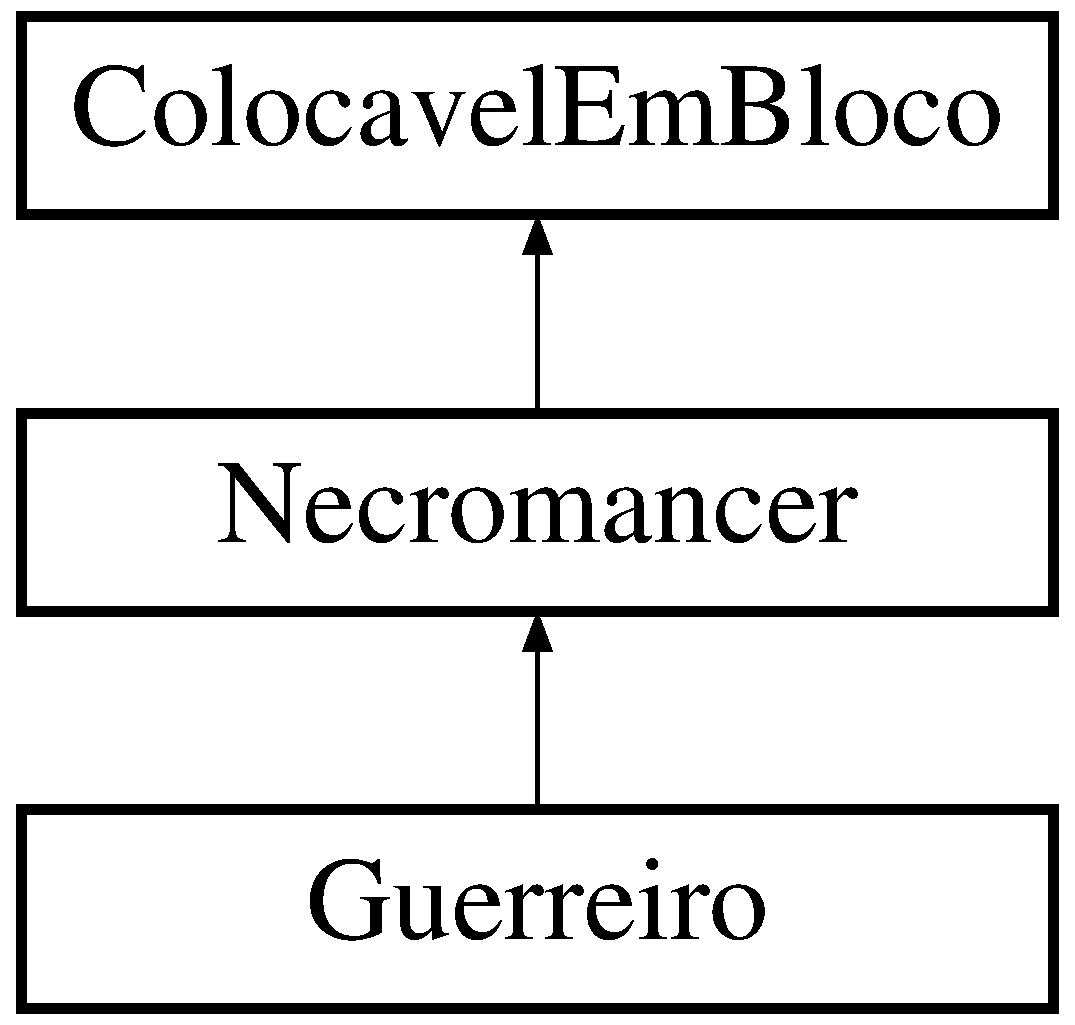
\includegraphics[height=3.000000cm]{class_guerreiro}
\end{center}
\end{figure}
\subsection*{Public Member Functions}
\begin{DoxyCompactItemize}
\item 
\mbox{\Hypertarget{class_guerreiro_a161ed48fa288b011c1c251520e811639}\label{class_guerreiro_a161ed48fa288b011c1c251520e811639}} 
\mbox{\hyperlink{class_guerreiro_a161ed48fa288b011c1c251520e811639}{Guerreiro}} ()
\begin{DoxyCompactList}\small\item\em Construct a new \mbox{\hyperlink{class_guerreiro}{Guerreiro}}\+:\+: \mbox{\hyperlink{class_guerreiro}{Guerreiro}} object. \end{DoxyCompactList}\end{DoxyCompactItemize}
\subsection*{Additional Inherited Members}


\subsection{Detailed Description}


Definition at line 56 of file Necromancer.\+hpp.



The documentation for this class was generated from the following files\+:\begin{DoxyCompactItemize}
\item 
include/\mbox{\hyperlink{_necromancer_8hpp}{Necromancer.\+hpp}}\item 
src/\mbox{\hyperlink{_necromancer_8cpp}{Necromancer.\+cpp}}\end{DoxyCompactItemize}

\hypertarget{class_mapa}{}\section{Mapa Class Reference}
\label{class_mapa}\index{Mapa@{Mapa}}
\subsection*{Public Member Functions}
\begin{DoxyCompactItemize}
\item 
\mbox{\hyperlink{class_mapa_ad722918f4e9150eb37d27de9f2847d5c}{Mapa}} (unsigned short, unsigned short)
\begin{DoxyCompactList}\small\item\em Construct a new \mbox{\hyperlink{class_mapa}{Mapa}}\+:\+: \mbox{\hyperlink{class_mapa}{Mapa}} object. \end{DoxyCompactList}\item 
bool \mbox{\hyperlink{class_mapa_aa07c1444720958b3efbc734d2691361d}{posicao\+\_\+valida}} (unsigned short, unsigned short)
\item 
bool \mbox{\hyperlink{class_mapa_a5bdde997d3c97c5b6fb7d37c124cdf93}{vazio}} (unsigned short, unsigned short)
\item 
bool \mbox{\hyperlink{class_mapa_a4dbab5cd3008b39687d8d2edb0ebacee}{inserir}} (\mbox{\hyperlink{class_colocavel_em_bloco}{Colocavel\+Em\+Bloco}} $\ast$, unsigned short, unsigned short)
\item 
\mbox{\hyperlink{class_colocavel_em_bloco}{Colocavel\+Em\+Bloco}} $\ast$ \mbox{\hyperlink{class_mapa_a52dbdf40a47afb56b1cb35dd1cb552f5}{ver}} (unsigned short, unsigned short)
\item 
\mbox{\hyperlink{class_colocavel_em_bloco}{Colocavel\+Em\+Bloco}} $\ast$ \mbox{\hyperlink{class_mapa_a8c216da0fb1514cb354c40b64d9af93a}{retirar}} (unsigned short, unsigned short)
\end{DoxyCompactItemize}
\subsection*{Public Attributes}
\begin{DoxyCompactItemize}
\item 
\mbox{\Hypertarget{class_mapa_a510e97a3b1705bd120220da7a1ce1cbf}\label{class_mapa_a510e97a3b1705bd120220da7a1ce1cbf}} 
Posicao {\bfseries cursor}
\item 
\mbox{\Hypertarget{class_mapa_ae1372f45e15677c1ac55e88e9cb1f240}\label{class_mapa_ae1372f45e15677c1ac55e88e9cb1f240}} 
Mapa\+De\+Blocos {\bfseries mapa}
\end{DoxyCompactItemize}


\subsection{Detailed Description}


Definition at line 25 of file Mapa.\+hpp.



\subsection{Constructor \& Destructor Documentation}
\mbox{\Hypertarget{class_mapa_ad722918f4e9150eb37d27de9f2847d5c}\label{class_mapa_ad722918f4e9150eb37d27de9f2847d5c}} 
\index{Mapa@{Mapa}!Mapa@{Mapa}}
\index{Mapa@{Mapa}!Mapa@{Mapa}}
\subsubsection{\texorpdfstring{Mapa()}{Mapa()}}
{\footnotesize\ttfamily Mapa\+::\+Mapa (\begin{DoxyParamCaption}\item[{unsigned short}]{X,  }\item[{unsigned short}]{Y }\end{DoxyParamCaption})}



Construct a new \mbox{\hyperlink{class_mapa}{Mapa}}\+:\+: \mbox{\hyperlink{class_mapa}{Mapa}} object. 


\begin{DoxyParams}{Parameters}
{\em X} & \\
\hline
{\em Y} & \\
\hline
\end{DoxyParams}


Definition at line 24 of file Mapa.\+cpp.


\begin{DoxyCode}
24                                              \{
25     this->tam\_x = X;
26     this->tam\_y = Y;
27     \textcolor{keywordtype}{int} i, j;
28     \textcolor{keywordflow}{for} (i = 0; i < X; i++)
29         \textcolor{keywordflow}{for} (j = 0; j < Y; j++)
30             this->mapa[std::make\_pair(i, j)] = \mbox{\hyperlink{class_bloco}{Bloco}}();
31 \}
\end{DoxyCode}


\subsection{Member Function Documentation}
\mbox{\Hypertarget{class_mapa_a4dbab5cd3008b39687d8d2edb0ebacee}\label{class_mapa_a4dbab5cd3008b39687d8d2edb0ebacee}} 
\index{Mapa@{Mapa}!inserir@{inserir}}
\index{inserir@{inserir}!Mapa@{Mapa}}
\subsubsection{\texorpdfstring{inserir()}{inserir()}}
{\footnotesize\ttfamily bool Mapa\+::inserir (\begin{DoxyParamCaption}\item[{\mbox{\hyperlink{class_colocavel_em_bloco}{Colocavel\+Em\+Bloco}} $\ast$}]{item,  }\item[{unsigned short}]{X,  }\item[{unsigned short}]{Y }\end{DoxyParamCaption})}


\begin{DoxyParams}{Parameters}
{\em item} & \\
\hline
{\em X} & \\
\hline
{\em Y} & \\
\hline
\end{DoxyParams}
\begin{DoxyReturn}{Returns}
true 

false 
\end{DoxyReturn}


Definition at line 68 of file Mapa.\+cpp.



References vazio().



Referenced by Controlador\+::criar\+\_\+necromancer(), Controlador\+::criar\+\_\+pilar(), and Controlador\+::novo\+\_\+jogo().


\begin{DoxyCode}
68                                                                              \{
69     \textcolor{keywordflow}{if} (!this->\mbox{\hyperlink{class_mapa_a5bdde997d3c97c5b6fb7d37c124cdf93}{vazio}}(X, Y)) \textcolor{keywordflow}{return} \textcolor{keyword}{false};
70 
71     this->mapa[std::make\_pair(X, Y)].preenche(item);
72     item->x = X;
73     item->y = Y;
74     \textcolor{keywordflow}{return} \textcolor{keyword}{true};
75 \}
\end{DoxyCode}
\mbox{\Hypertarget{class_mapa_aa07c1444720958b3efbc734d2691361d}\label{class_mapa_aa07c1444720958b3efbc734d2691361d}} 
\index{Mapa@{Mapa}!posicao\+\_\+valida@{posicao\+\_\+valida}}
\index{posicao\+\_\+valida@{posicao\+\_\+valida}!Mapa@{Mapa}}
\subsubsection{\texorpdfstring{posicao\+\_\+valida()}{posicao\_valida()}}
{\footnotesize\ttfamily bool Mapa\+::posicao\+\_\+valida (\begin{DoxyParamCaption}\item[{unsigned short}]{X,  }\item[{unsigned short}]{Y }\end{DoxyParamCaption})}


\begin{DoxyParams}{Parameters}
{\em X} & \\
\hline
{\em Y} & \\
\hline
\end{DoxyParams}
\begin{DoxyReturn}{Returns}
true 

false 
\end{DoxyReturn}


Definition at line 41 of file Mapa.\+cpp.



Referenced by Controlador\+::gerou\+\_\+combate(), Controlador\+::pode\+\_\+movimentar(), retirar(), vazio(), and ver().


\begin{DoxyCode}
41                                                             \{
42     \textcolor{keywordflow}{return} X < this->tam\_x && Y < this->tam\_y;
43 \}
\end{DoxyCode}
\mbox{\Hypertarget{class_mapa_a8c216da0fb1514cb354c40b64d9af93a}\label{class_mapa_a8c216da0fb1514cb354c40b64d9af93a}} 
\index{Mapa@{Mapa}!retirar@{retirar}}
\index{retirar@{retirar}!Mapa@{Mapa}}
\subsubsection{\texorpdfstring{retirar()}{retirar()}}
{\footnotesize\ttfamily \mbox{\hyperlink{class_colocavel_em_bloco}{Colocavel\+Em\+Bloco}} $\ast$ Mapa\+::retirar (\begin{DoxyParamCaption}\item[{unsigned short}]{X,  }\item[{unsigned short}]{Y }\end{DoxyParamCaption})}


\begin{DoxyParams}{Parameters}
{\em X} & \\
\hline
{\em Y} & \\
\hline
\end{DoxyParams}
\begin{DoxyReturn}{Returns}
Colocavel\+Em\+Bloco$\ast$ 
\end{DoxyReturn}


Definition at line 98 of file Mapa.\+cpp.



References posicao\+\_\+valida(), and vazio().



Referenced by Controlador\+::movimentar().


\begin{DoxyCode}
98                                                                   \{
99     \textcolor{keywordflow}{if} (this->\mbox{\hyperlink{class_mapa_a5bdde997d3c97c5b6fb7d37c124cdf93}{vazio}}(X, Y) || !this->\mbox{\hyperlink{class_mapa_aa07c1444720958b3efbc734d2691361d}{posicao\_valida}}(X, Y)) \textcolor{keywordflow}{return} \textcolor{keyword}{nullptr};
100     \mbox{\hyperlink{class_colocavel_em_bloco}{ColocavelEmBloco}} *conteudo = this->mapa[std::make\_pair(X, Y)].conteudo;
101     this->mapa[std::make\_pair(X, Y)].limpa();
102 
103     \textcolor{keywordflow}{return} conteudo;
104 \}
\end{DoxyCode}
\mbox{\Hypertarget{class_mapa_a5bdde997d3c97c5b6fb7d37c124cdf93}\label{class_mapa_a5bdde997d3c97c5b6fb7d37c124cdf93}} 
\index{Mapa@{Mapa}!vazio@{vazio}}
\index{vazio@{vazio}!Mapa@{Mapa}}
\subsubsection{\texorpdfstring{vazio()}{vazio()}}
{\footnotesize\ttfamily bool Mapa\+::vazio (\begin{DoxyParamCaption}\item[{unsigned short}]{X,  }\item[{unsigned short}]{Y }\end{DoxyParamCaption})}


\begin{DoxyParams}{Parameters}
{\em X} & \\
\hline
{\em Y} & \\
\hline
\end{DoxyParams}
\begin{DoxyReturn}{Returns}
true 

false 
\end{DoxyReturn}


Definition at line 53 of file Mapa.\+cpp.



References posicao\+\_\+valida().



Referenced by Controlador\+::criar\+\_\+necromancer(), Controlador\+::criar\+\_\+pilar(), Controlador\+::gerou\+\_\+combate(), inserir(), Controlador\+::matar(), Controlador\+::movimentar(), Controlador\+::pode\+\_\+movimentar(), retirar(), and ver().


\begin{DoxyCode}
53                                                    \{
54     \textcolor{keywordflow}{if} (!this->\mbox{\hyperlink{class_mapa_aa07c1444720958b3efbc734d2691361d}{posicao\_valida}}(X, Y)) \textcolor{keywordflow}{return} \textcolor{keyword}{false};
55 
56     \textcolor{keywordflow}{return} this->mapa[std::make\_pair(X, Y)].vazio;
57 \}
\end{DoxyCode}
\mbox{\Hypertarget{class_mapa_a52dbdf40a47afb56b1cb35dd1cb552f5}\label{class_mapa_a52dbdf40a47afb56b1cb35dd1cb552f5}} 
\index{Mapa@{Mapa}!ver@{ver}}
\index{ver@{ver}!Mapa@{Mapa}}
\subsubsection{\texorpdfstring{ver()}{ver()}}
{\footnotesize\ttfamily \mbox{\hyperlink{class_colocavel_em_bloco}{Colocavel\+Em\+Bloco}} $\ast$ Mapa\+::ver (\begin{DoxyParamCaption}\item[{unsigned short}]{X,  }\item[{unsigned short}]{Y }\end{DoxyParamCaption})}


\begin{DoxyParams}{Parameters}
{\em X} & \\
\hline
{\em Y} & \\
\hline
\end{DoxyParams}
\begin{DoxyReturn}{Returns}
Colocavel\+Em\+Bloco$\ast$ 
\end{DoxyReturn}


Definition at line 84 of file Mapa.\+cpp.



References posicao\+\_\+valida(), and vazio().



Referenced by Controlador\+::gerou\+\_\+combate(), Controlador\+::matar(), Controlador\+::movimentar(), Controlador\+::pode\+\_\+movimentar(), Controlador\+::realiza\+\_\+combate(), and Controlador\+::verifica\+\_\+combate().


\begin{DoxyCode}
84                                                               \{
85     \textcolor{keywordflow}{if} (this->\mbox{\hyperlink{class_mapa_a5bdde997d3c97c5b6fb7d37c124cdf93}{vazio}}(X, Y) || !this->\mbox{\hyperlink{class_mapa_aa07c1444720958b3efbc734d2691361d}{posicao\_valida}}(X, Y)) \textcolor{keywordflow}{return} \textcolor{keyword}{nullptr};
86     \mbox{\hyperlink{class_colocavel_em_bloco}{ColocavelEmBloco}} *conteudo = this->mapa[std::make\_pair(X, Y)].conteudo;
87 
88     \textcolor{keywordflow}{return} conteudo;
89 \}
\end{DoxyCode}


The documentation for this class was generated from the following files\+:\begin{DoxyCompactItemize}
\item 
include/\mbox{\hyperlink{_mapa_8hpp}{Mapa.\+hpp}}\item 
src/\mbox{\hyperlink{_mapa_8cpp}{Mapa.\+cpp}}\end{DoxyCompactItemize}

\hypertarget{class_metal}{}\section{Metal Class Reference}
\label{class_metal}\index{Metal@{Metal}}
Inheritance diagram for Metal\+:\begin{figure}[H]
\begin{center}
\leavevmode
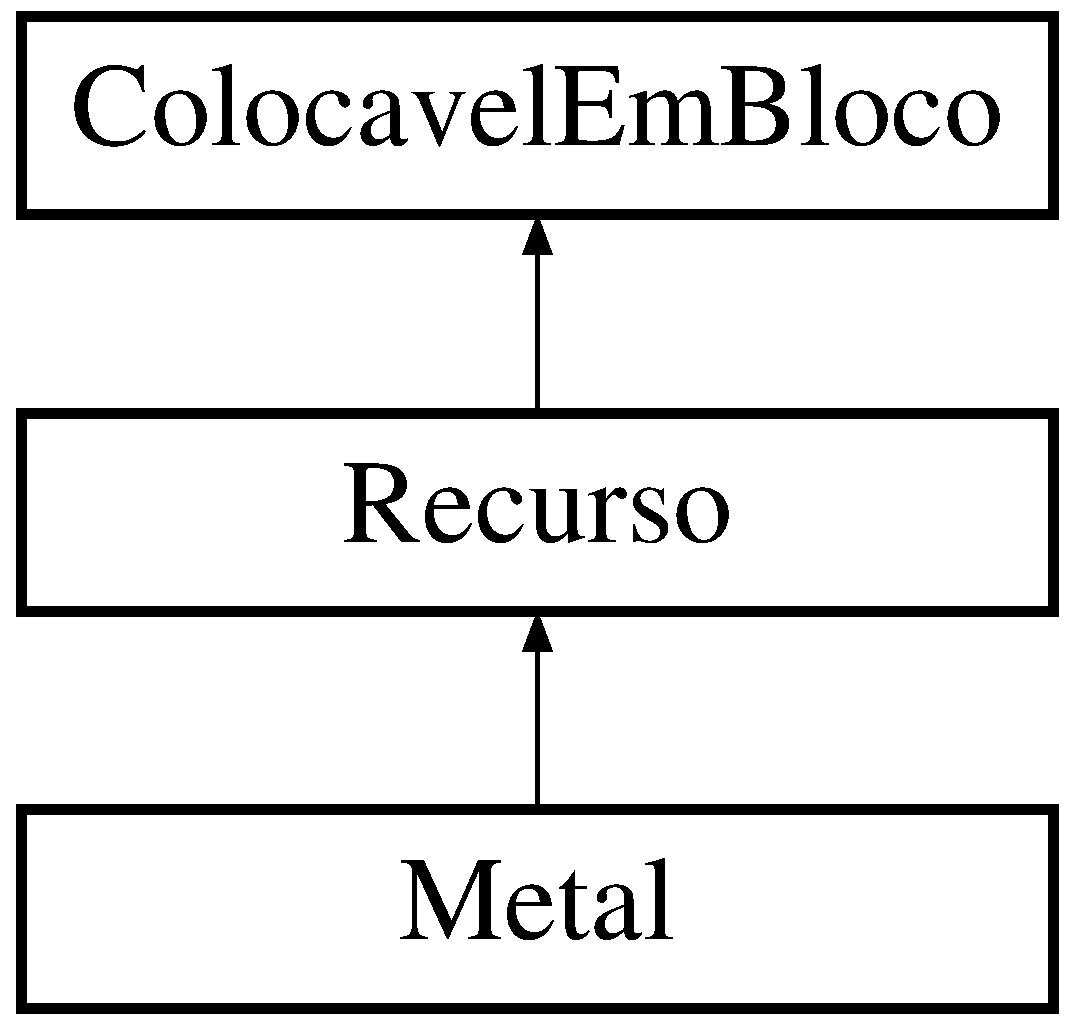
\includegraphics[height=3.000000cm]{class_metal}
\end{center}
\end{figure}
\subsection*{Public Member Functions}
\begin{DoxyCompactItemize}
\item 
\mbox{\Hypertarget{class_metal_a4439579b25694774c6e79daf71230524}\label{class_metal_a4439579b25694774c6e79daf71230524}} 
\mbox{\hyperlink{class_metal_a4439579b25694774c6e79daf71230524}{Metal}} ()
\begin{DoxyCompactList}\small\item\em Construct a new \mbox{\hyperlink{class_metal}{Metal}}\+:\+: \mbox{\hyperlink{class_metal}{Metal}} object. \end{DoxyCompactList}\end{DoxyCompactItemize}
\subsection*{Additional Inherited Members}


\subsection{Detailed Description}


Definition at line 37 of file Recurso.\+hpp.



The documentation for this class was generated from the following files\+:\begin{DoxyCompactItemize}
\item 
include/\mbox{\hyperlink{_recurso_8hpp}{Recurso.\+hpp}}\item 
src/\mbox{\hyperlink{_recurso_8cpp}{Recurso.\+cpp}}\end{DoxyCompactItemize}

\hypertarget{class_necromancer}{}\section{Necromancer Class Reference}
\label{class_necromancer}\index{Necromancer@{Necromancer}}
Inheritance diagram for Necromancer\+:\begin{figure}[H]
\begin{center}
\leavevmode
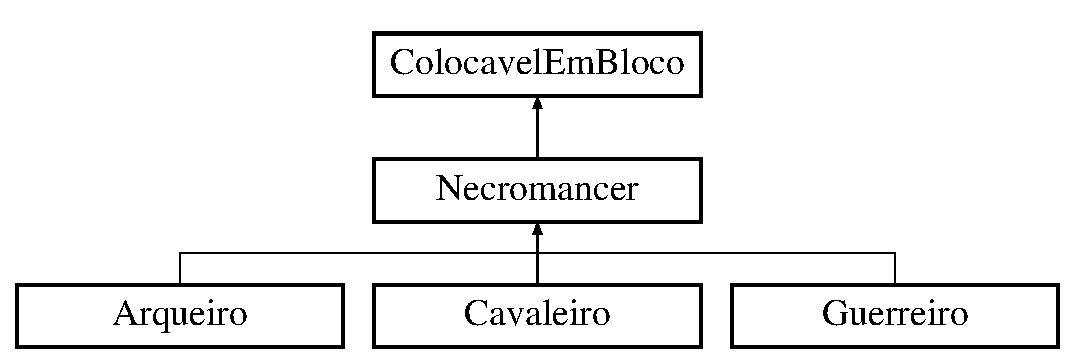
\includegraphics[height=3.000000cm]{class_necromancer}
\end{center}
\end{figure}
\subsection*{Public Member Functions}
\begin{DoxyCompactItemize}
\item 
\mbox{\Hypertarget{class_necromancer_a2d9f222048d7321295264900dd5879f9}\label{class_necromancer_a2d9f222048d7321295264900dd5879f9}} 
\mbox{\hyperlink{class_necromancer_a2d9f222048d7321295264900dd5879f9}{Necromancer}} ()
\begin{DoxyCompactList}\small\item\em Construct a new \mbox{\hyperlink{class_necromancer}{Necromancer}}\+:\+: \mbox{\hyperlink{class_necromancer}{Necromancer}} object. \end{DoxyCompactList}\item 
unsigned short \mbox{\hyperlink{class_necromancer_ae276261d4338078bb09b24e73c1abb5b}{multiplicador}} (Tipo\+Pilar tipo)
\item 
unsigned short \mbox{\hyperlink{class_necromancer_ad8a25efaa26240e028c893d1df80b067}{multiplicador}} (Tipo\+Necromancer tipo)
\item 
\mbox{\Hypertarget{class_necromancer_a8e7451787b08609862b19851bfb5e699}\label{class_necromancer_a8e7451787b08609862b19851bfb5e699}} 
bool {\bfseries handle\+Event} (S\+D\+L\+\_\+\+Event $\ast$e, int x, int y)
\end{DoxyCompactItemize}
\subsection*{Public Attributes}
\begin{DoxyCompactItemize}
\item 
\mbox{\Hypertarget{class_necromancer_a59c7606cb39566c863099344f8ab06ed}\label{class_necromancer_a59c7606cb39566c863099344f8ab06ed}} 
unsigned short {\bfseries mp}
\item 
\mbox{\Hypertarget{class_necromancer_ad2db9dae93163aa8506be6ded7861906}\label{class_necromancer_ad2db9dae93163aa8506be6ded7861906}} 
Tipo\+Necromancer {\bfseries tipo\+\_\+necromancer}
\end{DoxyCompactItemize}


\subsection{Detailed Description}


Definition at line 39 of file Necromancer.\+hpp.



\subsection{Member Function Documentation}
\mbox{\Hypertarget{class_necromancer_ae276261d4338078bb09b24e73c1abb5b}\label{class_necromancer_ae276261d4338078bb09b24e73c1abb5b}} 
\index{Necromancer@{Necromancer}!multiplicador@{multiplicador}}
\index{multiplicador@{multiplicador}!Necromancer@{Necromancer}}
\subsubsection{\texorpdfstring{multiplicador()}{multiplicador()}\hspace{0.1cm}{\footnotesize\ttfamily [1/2]}}
{\footnotesize\ttfamily unsigned short Necromancer\+::multiplicador (\begin{DoxyParamCaption}\item[{Tipo\+Pilar}]{tipo }\end{DoxyParamCaption})}


\begin{DoxyParams}{Parameters}
{\em tipo} & \\
\hline
\end{DoxyParams}
\begin{DoxyReturn}{Returns}
unsigned short 
\end{DoxyReturn}


Definition at line 97 of file Necromancer.\+cpp.


\begin{DoxyCode}
97                                                         \{
98     \textcolor{keywordflow}{if} (this->tipo\_necromancer == TipoNecromancer::ARQUEIRO) \{
99         \textcolor{keywordflow}{if} (tipo == TipoPilar::ESPADA)
100             \textcolor{keywordflow}{return} ARCO\_ESPADA\_ATQ\_MULTIPLICADOR;
101 
102         \textcolor{keywordflow}{if} (tipo == TipoPilar::LANCA)
103             \textcolor{keywordflow}{return} ARCO\_LANCA\_ATQ\_MULTIPLICADOR;
104 
105         \textcolor{keywordflow}{if} (tipo == TipoPilar::ARCO)
106             \textcolor{keywordflow}{return} ARCO\_ARCO\_ATQ\_MULTIPLICADOR;
107     \}
108     \textcolor{keywordflow}{if} (this->tipo\_necromancer == TipoNecromancer::CAVALEIRO) \{
109         \textcolor{keywordflow}{if} (tipo == TipoPilar::ESPADA)
110             \textcolor{keywordflow}{return} LANCA\_ESPADA\_ATQ\_MULTIPLICADOR;
111 
112         \textcolor{keywordflow}{if} (tipo == TipoPilar::LANCA)
113             \textcolor{keywordflow}{return} LANCA\_LANCA\_ATQ\_MULTIPLICADOR;
114 
115         \textcolor{keywordflow}{if} (tipo == TipoPilar::ARCO)
116             \textcolor{keywordflow}{return} LANCA\_ARCO\_ATQ\_MULTIPLICADOR;
117     \}
118     \textcolor{keywordflow}{if} (this->tipo\_necromancer == TipoNecromancer::GUERREIRO) \{
119         \textcolor{keywordflow}{if} (tipo == TipoPilar::ESPADA)
120             \textcolor{keywordflow}{return} ESPADA\_ESPADA\_ATQ\_MULTIPLICADOR;
121 
122         \textcolor{keywordflow}{if} (tipo == TipoPilar::LANCA)
123             \textcolor{keywordflow}{return} ESPADA\_LANCA\_ATQ\_MULTIPLICADOR;
124 
125         \textcolor{keywordflow}{if} (tipo == TipoPilar::ARCO)
126             \textcolor{keywordflow}{return} ESPADA\_ARCO\_ATQ\_MULTIPLICADOR;
127     \}
128     \textcolor{keywordflow}{return} 0;
129 \}
\end{DoxyCode}
\mbox{\Hypertarget{class_necromancer_ad8a25efaa26240e028c893d1df80b067}\label{class_necromancer_ad8a25efaa26240e028c893d1df80b067}} 
\index{Necromancer@{Necromancer}!multiplicador@{multiplicador}}
\index{multiplicador@{multiplicador}!Necromancer@{Necromancer}}
\subsubsection{\texorpdfstring{multiplicador()}{multiplicador()}\hspace{0.1cm}{\footnotesize\ttfamily [2/2]}}
{\footnotesize\ttfamily unsigned short Necromancer\+::multiplicador (\begin{DoxyParamCaption}\item[{Tipo\+Necromancer}]{tipo }\end{DoxyParamCaption})}


\begin{DoxyParams}{Parameters}
{\em tipo} & \\
\hline
\end{DoxyParams}
\begin{DoxyReturn}{Returns}
unsigned short 
\end{DoxyReturn}


Definition at line 137 of file Necromancer.\+cpp.


\begin{DoxyCode}
137                                                               \{
138     \textcolor{keywordflow}{if} (this->tipo\_necromancer == TipoNecromancer::ARQUEIRO) \{
139         \textcolor{keywordflow}{if} (tipo == TipoNecromancer::GUERREIRO)
140             \textcolor{keywordflow}{return} ARCO\_ESPADA\_ATQ\_MULTIPLICADOR;
141 
142         \textcolor{keywordflow}{if} (tipo == TipoNecromancer::CAVALEIRO)
143             \textcolor{keywordflow}{return} ARCO\_LANCA\_ATQ\_MULTIPLICADOR;
144 
145         \textcolor{keywordflow}{if} (tipo == TipoNecromancer::ARQUEIRO)
146             \textcolor{keywordflow}{return} ARCO\_ARCO\_ATQ\_MULTIPLICADOR;
147     \}
148     \textcolor{keywordflow}{if} (this->tipo\_necromancer == TipoNecromancer::CAVALEIRO) \{
149         \textcolor{keywordflow}{if} (tipo == TipoNecromancer::GUERREIRO)
150             \textcolor{keywordflow}{return} LANCA\_ESPADA\_ATQ\_MULTIPLICADOR;
151 
152         \textcolor{keywordflow}{if} (tipo == TipoNecromancer::CAVALEIRO)
153             \textcolor{keywordflow}{return} LANCA\_LANCA\_ATQ\_MULTIPLICADOR;
154 
155         \textcolor{keywordflow}{if} (tipo == TipoNecromancer::ARQUEIRO)
156             \textcolor{keywordflow}{return} LANCA\_ARCO\_ATQ\_MULTIPLICADOR;
157     \}
158     \textcolor{keywordflow}{if} (this->tipo\_necromancer == TipoNecromancer::GUERREIRO) \{
159         \textcolor{keywordflow}{if} (tipo == TipoNecromancer::GUERREIRO)
160             \textcolor{keywordflow}{return} ESPADA\_ESPADA\_ATQ\_MULTIPLICADOR;
161 
162         \textcolor{keywordflow}{if} (tipo == TipoNecromancer::CAVALEIRO)
163             \textcolor{keywordflow}{return} ESPADA\_LANCA\_ATQ\_MULTIPLICADOR;
164 
165         \textcolor{keywordflow}{if} (tipo == TipoNecromancer::ARQUEIRO)
166             \textcolor{keywordflow}{return} ESPADA\_ARCO\_ATQ\_MULTIPLICADOR;
167     \}
168     \textcolor{keywordflow}{return} 0;
169 \}
\end{DoxyCode}


The documentation for this class was generated from the following files\+:\begin{DoxyCompactItemize}
\item 
include/\mbox{\hyperlink{_necromancer_8hpp}{Necromancer.\+hpp}}\item 
src/\mbox{\hyperlink{_necromancer_8cpp}{Necromancer.\+cpp}}\end{DoxyCompactItemize}

\hypertarget{class_ossos}{}\section{Ossos Class Reference}
\label{class_ossos}\index{Ossos@{Ossos}}
Inheritance diagram for Ossos\+:\begin{figure}[H]
\begin{center}
\leavevmode
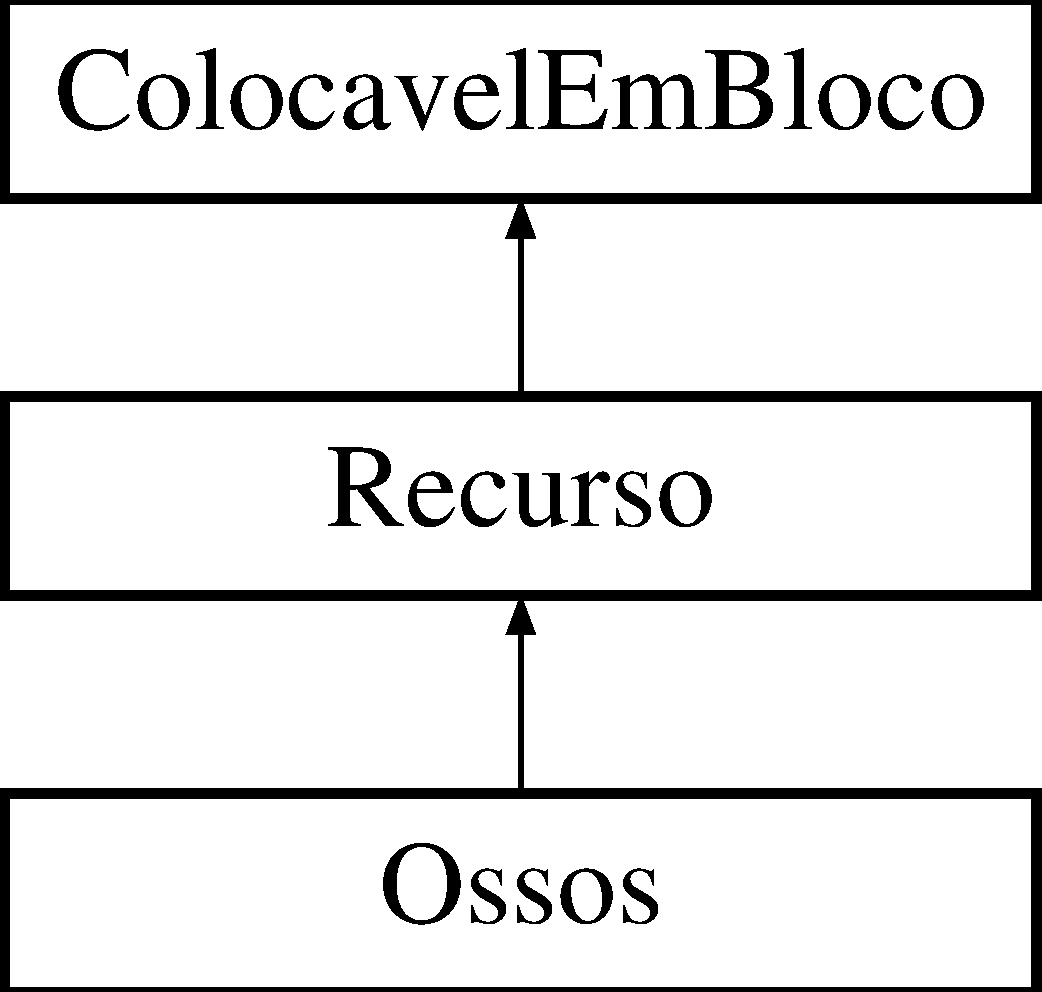
\includegraphics[height=3.000000cm]{class_ossos}
\end{center}
\end{figure}
\subsection*{Public Member Functions}
\begin{DoxyCompactItemize}
\item 
\mbox{\Hypertarget{class_ossos_a37b5a58e92f03645c8ae597de25e3df0}\label{class_ossos_a37b5a58e92f03645c8ae597de25e3df0}} 
\mbox{\hyperlink{class_ossos_a37b5a58e92f03645c8ae597de25e3df0}{Ossos}} ()
\begin{DoxyCompactList}\small\item\em Construct a new \mbox{\hyperlink{class_ossos}{Ossos}}\+:\+: \mbox{\hyperlink{class_ossos}{Ossos}} object. \end{DoxyCompactList}\end{DoxyCompactItemize}
\subsection*{Additional Inherited Members}


\subsection{Detailed Description}


Definition at line 44 of file Recurso.\+hpp.



The documentation for this class was generated from the following files\+:\begin{DoxyCompactItemize}
\item 
include/\mbox{\hyperlink{_recurso_8hpp}{Recurso.\+hpp}}\item 
src/\mbox{\hyperlink{_recurso_8cpp}{Recurso.\+cpp}}\end{DoxyCompactItemize}

\hypertarget{class_pilar}{}\section{Pilar Class Reference}
\label{class_pilar}\index{Pilar@{Pilar}}
Inheritance diagram for Pilar\+:\begin{figure}[H]
\begin{center}
\leavevmode
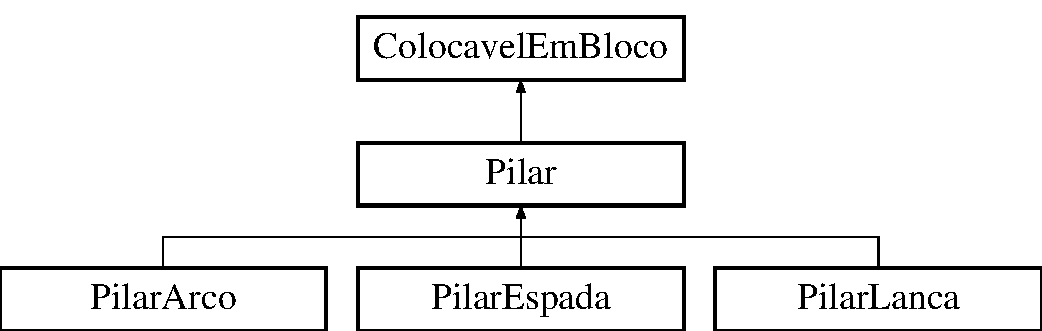
\includegraphics[height=3.000000cm]{class_pilar}
\end{center}
\end{figure}
\subsection*{Public Member Functions}
\begin{DoxyCompactItemize}
\item 
\mbox{\Hypertarget{class_pilar_a0a45a9e317ace22fda66c43b1987104d}\label{class_pilar_a0a45a9e317ace22fda66c43b1987104d}} 
\mbox{\hyperlink{class_pilar_a0a45a9e317ace22fda66c43b1987104d}{Pilar}} ()
\begin{DoxyCompactList}\small\item\em Construct a new \mbox{\hyperlink{class_pilar}{Pilar}}\+:\+: \mbox{\hyperlink{class_pilar}{Pilar}} object. \end{DoxyCompactList}\item 
\mbox{\Hypertarget{class_pilar_a75256cfabc394e62abe757acb86ddb76}\label{class_pilar_a75256cfabc394e62abe757acb86ddb76}} 
bool {\bfseries handle\+Event} (S\+D\+L\+\_\+\+Event $\ast$e, int position\+\_\+x, int position\+\_\+y)
\end{DoxyCompactItemize}
\subsection*{Public Attributes}
\begin{DoxyCompactItemize}
\item 
\mbox{\Hypertarget{class_pilar_ad4148c5c8898c3e857d0140bdd362c84}\label{class_pilar_ad4148c5c8898c3e857d0140bdd362c84}} 
unsigned short {\bfseries hp}
\item 
\mbox{\Hypertarget{class_pilar_a2c1911ab606a59529bc1dcedb27c986c}\label{class_pilar_a2c1911ab606a59529bc1dcedb27c986c}} 
Tipo\+Pilar {\bfseries tipo\+\_\+pilar}
\end{DoxyCompactItemize}


\subsection{Detailed Description}


Definition at line 28 of file Pilar.\+hpp.



The documentation for this class was generated from the following files\+:\begin{DoxyCompactItemize}
\item 
include/\mbox{\hyperlink{_pilar_8hpp}{Pilar.\+hpp}}\item 
src/\mbox{\hyperlink{_pilar_8cpp}{Pilar.\+cpp}}\end{DoxyCompactItemize}

\hypertarget{class_pilar_arco}{}\section{Pilar\+Arco Class Reference}
\label{class_pilar_arco}\index{Pilar\+Arco@{Pilar\+Arco}}
Inheritance diagram for Pilar\+Arco\+:\begin{figure}[H]
\begin{center}
\leavevmode
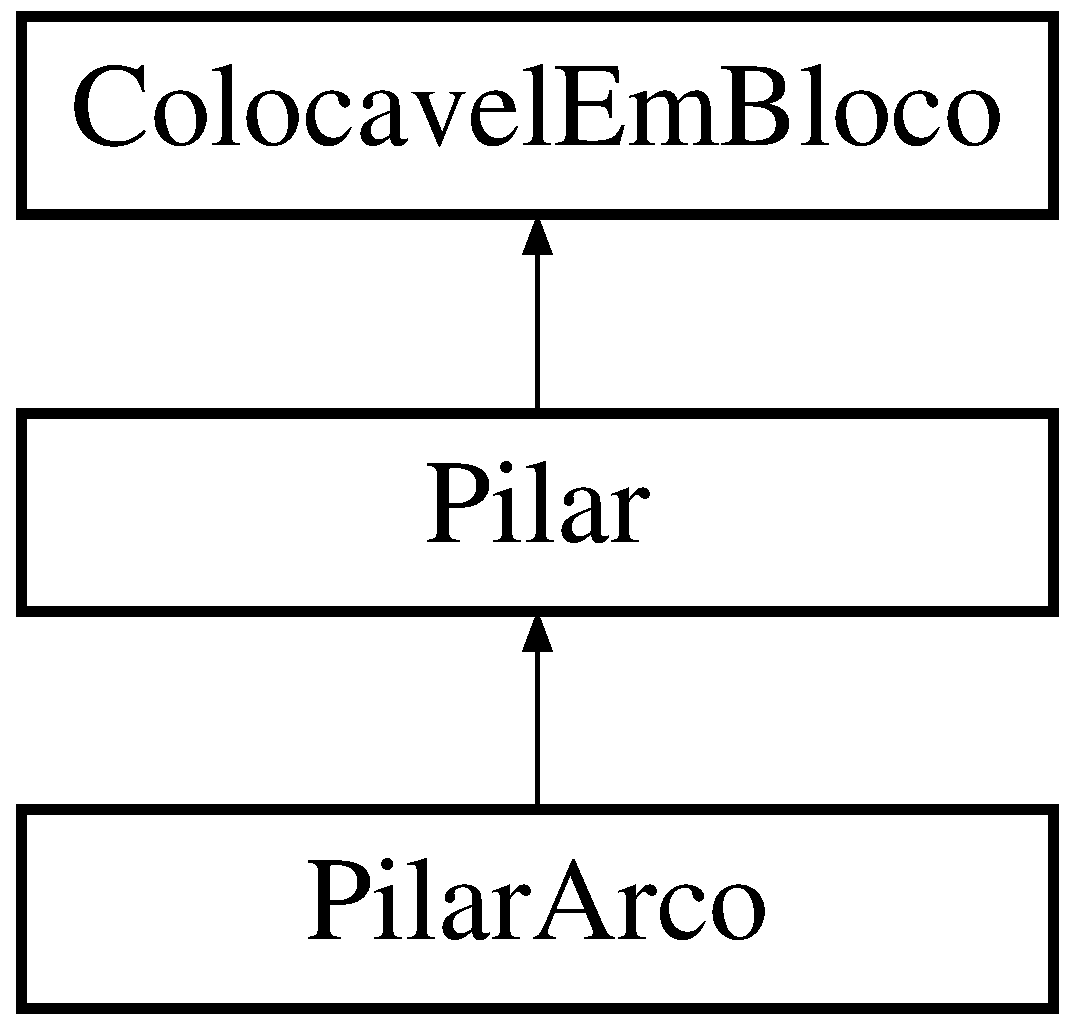
\includegraphics[height=3.000000cm]{class_pilar_arco}
\end{center}
\end{figure}
\subsection*{Public Member Functions}
\begin{DoxyCompactItemize}
\item 
\mbox{\Hypertarget{class_pilar_arco_a356e18041ea4a8e096327e591663157b}\label{class_pilar_arco_a356e18041ea4a8e096327e591663157b}} 
\mbox{\hyperlink{class_pilar_arco_a356e18041ea4a8e096327e591663157b}{Pilar\+Arco}} ()
\begin{DoxyCompactList}\small\item\em Construct a new \mbox{\hyperlink{class_pilar}{Pilar}} Arco\+:\+: \mbox{\hyperlink{class_pilar}{Pilar}} Arco object. \end{DoxyCompactList}\end{DoxyCompactItemize}
\subsection*{Additional Inherited Members}


\subsection{Detailed Description}


Definition at line 52 of file Pilar.\+hpp.



The documentation for this class was generated from the following files\+:\begin{DoxyCompactItemize}
\item 
include/\mbox{\hyperlink{_pilar_8hpp}{Pilar.\+hpp}}\item 
src/\mbox{\hyperlink{_pilar_8cpp}{Pilar.\+cpp}}\end{DoxyCompactItemize}

\hypertarget{class_pilar_espada}{}\section{Pilar\+Espada Class Reference}
\label{class_pilar_espada}\index{Pilar\+Espada@{Pilar\+Espada}}
Inheritance diagram for Pilar\+Espada\+:\begin{figure}[H]
\begin{center}
\leavevmode
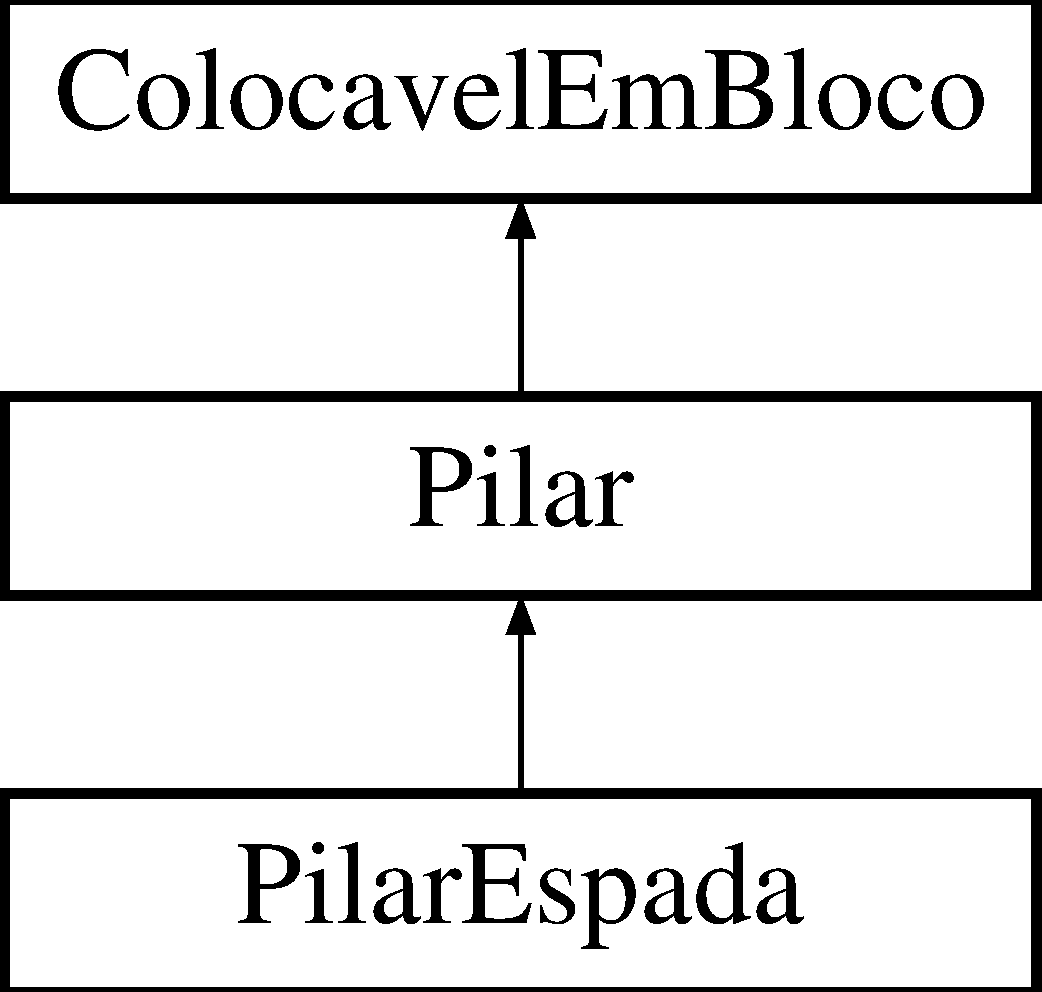
\includegraphics[height=3.000000cm]{class_pilar_espada}
\end{center}
\end{figure}
\subsection*{Public Member Functions}
\begin{DoxyCompactItemize}
\item 
\mbox{\Hypertarget{class_pilar_espada_abacf1e7d96b647406acb6e9630cd0425}\label{class_pilar_espada_abacf1e7d96b647406acb6e9630cd0425}} 
\mbox{\hyperlink{class_pilar_espada_abacf1e7d96b647406acb6e9630cd0425}{Pilar\+Espada}} ()
\begin{DoxyCompactList}\small\item\em Construct a new \mbox{\hyperlink{class_pilar}{Pilar}} Espada\+:\+: \mbox{\hyperlink{class_pilar}{Pilar}} Espada object. \end{DoxyCompactList}\end{DoxyCompactItemize}
\subsection*{Additional Inherited Members}


\subsection{Detailed Description}


Definition at line 38 of file Pilar.\+hpp.



The documentation for this class was generated from the following files\+:\begin{DoxyCompactItemize}
\item 
include/\mbox{\hyperlink{_pilar_8hpp}{Pilar.\+hpp}}\item 
src/\mbox{\hyperlink{_pilar_8cpp}{Pilar.\+cpp}}\end{DoxyCompactItemize}

\hypertarget{class_pilar_lanca}{}\section{Pilar\+Lanca Class Reference}
\label{class_pilar_lanca}\index{Pilar\+Lanca@{Pilar\+Lanca}}
Inheritance diagram for Pilar\+Lanca\+:\begin{figure}[H]
\begin{center}
\leavevmode
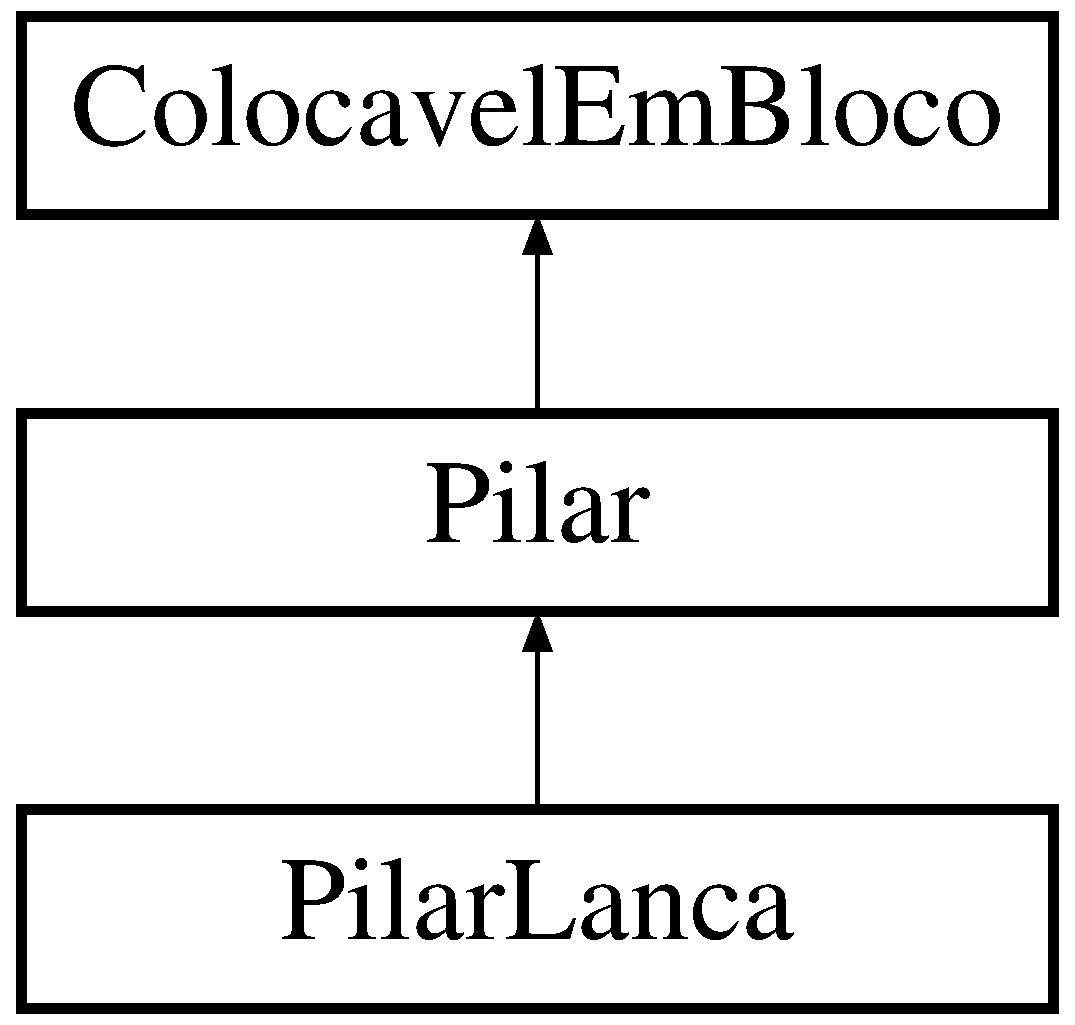
\includegraphics[height=3.000000cm]{class_pilar_lanca}
\end{center}
\end{figure}
\subsection*{Public Member Functions}
\begin{DoxyCompactItemize}
\item 
\mbox{\Hypertarget{class_pilar_lanca_a8763d3329a35b0253460f8d7b4b3fc7a}\label{class_pilar_lanca_a8763d3329a35b0253460f8d7b4b3fc7a}} 
\mbox{\hyperlink{class_pilar_lanca_a8763d3329a35b0253460f8d7b4b3fc7a}{Pilar\+Lanca}} ()
\begin{DoxyCompactList}\small\item\em Construct a new \mbox{\hyperlink{class_pilar}{Pilar}} Lanca\+:\+: \mbox{\hyperlink{class_pilar}{Pilar}} Lanca object. \end{DoxyCompactList}\end{DoxyCompactItemize}
\subsection*{Additional Inherited Members}


\subsection{Detailed Description}


Definition at line 45 of file Pilar.\+hpp.



The documentation for this class was generated from the following files\+:\begin{DoxyCompactItemize}
\item 
include/\mbox{\hyperlink{_pilar_8hpp}{Pilar.\+hpp}}\item 
src/\mbox{\hyperlink{_pilar_8cpp}{Pilar.\+cpp}}\end{DoxyCompactItemize}

\hypertarget{class_player}{}\section{Player Class Reference}
\label{class_player}\index{Player@{Player}}
\subsection*{Public Member Functions}
\begin{DoxyCompactItemize}
\item 
\mbox{\Hypertarget{class_player_affe0cc3cb714f6deb4e62f0c0d3f1fd8}\label{class_player_affe0cc3cb714f6deb4e62f0c0d3f1fd8}} 
\mbox{\hyperlink{class_player_affe0cc3cb714f6deb4e62f0c0d3f1fd8}{Player}} ()
\begin{DoxyCompactList}\small\item\em Construct a new \mbox{\hyperlink{class_player}{Player}}\+:\+: \mbox{\hyperlink{class_player}{Player}} object. \end{DoxyCompactList}\item 
bool \mbox{\hyperlink{class_player_a118c76695a9c1f362a5371381bfe5be3}{criar\+\_\+necromancer}} (Tipo\+Necromancer)
\item 
bool \mbox{\hyperlink{class_player_a23fda6bb2c90d8033dc6ae07d1f27964}{criar\+\_\+pilar}} (Tipo\+Pilar)
\item 
bool \mbox{\hyperlink{class_player_a063de6da853c618adcf8392ba639327c}{tem\+\_\+pilar}} (Tipo\+Pilar)
\item 
bool \mbox{\hyperlink{class_player_aeff8c71e2c3e1a7529ec2190de0ac4cd}{tem\+\_\+necromancer}} (Tipo\+Necromancer)
\item 
\mbox{\hyperlink{class_pilar}{Pilar}} $\ast$ \mbox{\hyperlink{class_player_aa953125244cebb04b2363ae102c5fbf6}{pilar}} (Tipo\+Pilar)
\item 
\mbox{\hyperlink{class_necromancer}{Necromancer}} $\ast$ \mbox{\hyperlink{class_player_a560ffc698994e73527433dd2bf4d2c0d}{necromancer}} (Tipo\+Necromancer)
\item 
bool \mbox{\hyperlink{class_player_a66d2bc18dfc9b913109761a95126f086}{captar\+\_\+recurso}} (Tipo\+Recurso)
\item 
\mbox{\Hypertarget{class_player_a2e69197c9ec7cebcc4e2a618c0342fbb}\label{class_player_a2e69197c9ec7cebcc4e2a618c0342fbb}} 
void {\bfseries muda\+\_\+time} ()
\item 
bool \mbox{\hyperlink{class_player_aad208bab9f9f88af5ac34ebe7c31dc61}{perdeu\+\_\+jogo}} ()
\item 
unsigned short \mbox{\hyperlink{class_player_a945277689283bc50bd3afef306bf9740}{pontuacao}} ()
\item 
void \mbox{\hyperlink{class_player_a7086da1dce5a9de1c2cf29a15ace5a7d}{print\+\_\+recursos}} (const char $\ast$)
\end{DoxyCompactItemize}
\subsection*{Public Attributes}
\begin{DoxyCompactItemize}
\item 
\mbox{\Hypertarget{class_player_a953244bbf0e0326076c22ba47c11a7cb}\label{class_player_a953244bbf0e0326076c22ba47c11a7cb}} 
unsigned short {\bfseries time}
\item 
\mbox{\Hypertarget{class_player_a33608a1ac91b463c5d4f0d75e6ed8724}\label{class_player_a33608a1ac91b463c5d4f0d75e6ed8724}} 
unsigned short {\bfseries metal}
\item 
\mbox{\Hypertarget{class_player_a147e27fdd4a9e19654ed924e14eced3a}\label{class_player_a147e27fdd4a9e19654ed924e14eced3a}} 
unsigned short {\bfseries ossos}
\item 
\mbox{\Hypertarget{class_player_a22564346bf7ddc4a9d6c99a265459067}\label{class_player_a22564346bf7ddc4a9d6c99a265459067}} 
\mbox{\hyperlink{class_guerreiro}{Guerreiro}} {\bfseries guerreiro}
\item 
\mbox{\Hypertarget{class_player_a92dffc00e1f3e6ad24bd0e9432f336cf}\label{class_player_a92dffc00e1f3e6ad24bd0e9432f336cf}} 
\mbox{\hyperlink{class_cavaleiro}{Cavaleiro}} {\bfseries cavaleiro}
\item 
\mbox{\Hypertarget{class_player_a9aeeec934470acf8f4eda1841abf4ed2}\label{class_player_a9aeeec934470acf8f4eda1841abf4ed2}} 
\mbox{\hyperlink{class_arqueiro}{Arqueiro}} {\bfseries arqueiro}
\item 
\mbox{\Hypertarget{class_player_a1b5158c5e932c8f782bb249680188301}\label{class_player_a1b5158c5e932c8f782bb249680188301}} 
\mbox{\hyperlink{class_pilar_espada}{Pilar\+Espada}} {\bfseries pilar\+\_\+espada}
\item 
\mbox{\Hypertarget{class_player_a2b30942a91b8d0342ec6e00d1f3a32f6}\label{class_player_a2b30942a91b8d0342ec6e00d1f3a32f6}} 
\mbox{\hyperlink{class_pilar_arco}{Pilar\+Arco}} {\bfseries pilar\+\_\+arco}
\item 
\mbox{\Hypertarget{class_player_a7b3f7a6b8ca2194cfb0af6dc783d790c}\label{class_player_a7b3f7a6b8ca2194cfb0af6dc783d790c}} 
\mbox{\hyperlink{class_pilar_lanca}{Pilar\+Lanca}} {\bfseries pilar\+\_\+lanca}
\end{DoxyCompactItemize}


\subsection{Detailed Description}


Definition at line 24 of file Player.\+hpp.



\subsection{Member Function Documentation}
\mbox{\Hypertarget{class_player_a66d2bc18dfc9b913109761a95126f086}\label{class_player_a66d2bc18dfc9b913109761a95126f086}} 
\index{Player@{Player}!captar\+\_\+recurso@{captar\+\_\+recurso}}
\index{captar\+\_\+recurso@{captar\+\_\+recurso}!Player@{Player}}
\subsubsection{\texorpdfstring{captar\+\_\+recurso()}{captar\_recurso()}}
{\footnotesize\ttfamily bool Player\+::captar\+\_\+recurso (\begin{DoxyParamCaption}\item[{Tipo\+Recurso}]{rec }\end{DoxyParamCaption})}


\begin{DoxyParams}{Parameters}
{\em rec} & \\
\hline
\end{DoxyParams}
\begin{DoxyReturn}{Returns}
true 

false 
\end{DoxyReturn}


Definition at line 79 of file Player.\+cpp.


\begin{DoxyCode}
79                                            \{
80     \textcolor{keywordflow}{if} (rec == TipoRecurso::METAL) \{
81         this->metal = this->metal + QUANTIDADE\_METAL\_POR\_ITEM;
82     \}
83     \textcolor{keywordflow}{if} (rec == TipoRecurso::OSSOS) \{
84         this->ossos = this->ossos + QUANTIDADE\_OSSOS\_POR\_ITEM;
85     \}
86     \textcolor{keywordflow}{return} \textcolor{keyword}{true};
87 \}
\end{DoxyCode}
\mbox{\Hypertarget{class_player_a118c76695a9c1f362a5371381bfe5be3}\label{class_player_a118c76695a9c1f362a5371381bfe5be3}} 
\index{Player@{Player}!criar\+\_\+necromancer@{criar\+\_\+necromancer}}
\index{criar\+\_\+necromancer@{criar\+\_\+necromancer}!Player@{Player}}
\subsubsection{\texorpdfstring{criar\+\_\+necromancer()}{criar\_necromancer()}}
{\footnotesize\ttfamily bool Player\+::criar\+\_\+necromancer (\begin{DoxyParamCaption}\item[{Tipo\+Necromancer}]{nec }\end{DoxyParamCaption})}


\begin{DoxyParams}{Parameters}
{\em nec} & \\
\hline
\end{DoxyParams}
\begin{DoxyReturn}{Returns}
true 

false 
\end{DoxyReturn}


Definition at line 205 of file Player.\+cpp.



Referenced by Controlador\+::criar\+\_\+necromancer(), and Controlador\+::fortalecer\+\_\+necromancer().


\begin{DoxyCode}
205                                                   \{
206     \textcolor{keywordflow}{if} (nec == TipoNecromancer::GUERREIRO) \{
207         \textcolor{keywordflow}{if} (!this->pilar\_espada.vivo)
208             \textcolor{keywordflow}{return} \textcolor{keyword}{false};
209         \textcolor{keywordflow}{if} (this->ossos < OSSOS\_CRIAR\_GUERREIRO)
210             \textcolor{keywordflow}{return} \textcolor{keyword}{false};
211 
212         this->ossos -= OSSOS\_CRIAR\_GUERREIRO;
213         \textcolor{keywordflow}{if} (!this->guerreiro.vivo) \{
214             this->guerreiro.\mbox{\hyperlink{class_colocavel_em_bloco_a82f12304bcb919f4fe3fc765d00a3d0f}{revive}}();
215             this->guerreiro.mp = MP\_INICIAL\_GUERREIRO;
216         \} \textcolor{keywordflow}{else} \{
217             this->guerreiro.mp += MP\_INICIAL\_GUERREIRO;
218         \}
219     \}
220 
221     \textcolor{keywordflow}{if} (nec == TipoNecromancer::CAVALEIRO) \{
222         \textcolor{keywordflow}{if} (!this->pilar\_lanca.vivo)
223             \textcolor{keywordflow}{return} \textcolor{keyword}{false};
224         \textcolor{keywordflow}{if} (this->ossos < OSSOS\_CRIAR\_CAVALEIRO)
225             \textcolor{keywordflow}{return} \textcolor{keyword}{false};
226 
227         this->ossos -= OSSOS\_CRIAR\_CAVALEIRO;
228 
229         \textcolor{keywordflow}{if} (!this->cavaleiro.vivo) \{
230             this->cavaleiro.\mbox{\hyperlink{class_colocavel_em_bloco_a82f12304bcb919f4fe3fc765d00a3d0f}{revive}}();
231             this->cavaleiro.mp = MP\_INICIAL\_CAVALEIRO;
232         \} \textcolor{keywordflow}{else} \{
233             this->cavaleiro.mp += MP\_INICIAL\_CAVALEIRO;
234         \}
235     \}
236 
237     \textcolor{keywordflow}{if} (nec == TipoNecromancer::ARQUEIRO) \{
238         \textcolor{keywordflow}{if} (!this->pilar\_arco.vivo)
239             \textcolor{keywordflow}{return} \textcolor{keyword}{false};
240         \textcolor{keywordflow}{if} (this->ossos < OSSOS\_CRIAR\_ARQUEIRO)
241             \textcolor{keywordflow}{return} \textcolor{keyword}{false};
242 
243         this->ossos -= OSSOS\_CRIAR\_ARQUEIRO;
244         \textcolor{keywordflow}{if} (!this->arqueiro.vivo) \{
245             this->arqueiro.\mbox{\hyperlink{class_colocavel_em_bloco_a82f12304bcb919f4fe3fc765d00a3d0f}{revive}}();
246             this->arqueiro.mp = MP\_INICIAL\_ARQUEIRO;
247         \} \textcolor{keywordflow}{else} \{
248             this->arqueiro.mp += MP\_INICIAL\_ARQUEIRO;
249         \}
250     \}
251 
252     \textcolor{keywordflow}{return} \textcolor{keyword}{true};
253 \}
\end{DoxyCode}
\mbox{\Hypertarget{class_player_a23fda6bb2c90d8033dc6ae07d1f27964}\label{class_player_a23fda6bb2c90d8033dc6ae07d1f27964}} 
\index{Player@{Player}!criar\+\_\+pilar@{criar\+\_\+pilar}}
\index{criar\+\_\+pilar@{criar\+\_\+pilar}!Player@{Player}}
\subsubsection{\texorpdfstring{criar\+\_\+pilar()}{criar\_pilar()}}
{\footnotesize\ttfamily bool Player\+::criar\+\_\+pilar (\begin{DoxyParamCaption}\item[{Tipo\+Pilar}]{pil }\end{DoxyParamCaption})}


\begin{DoxyParams}{Parameters}
{\em pil} & \\
\hline
\end{DoxyParams}
\begin{DoxyReturn}{Returns}
true 

false 
\end{DoxyReturn}


Definition at line 156 of file Player.\+cpp.



Referenced by Controlador\+::criar\+\_\+pilar(), and Controlador\+::fortalecer\+\_\+pilar().


\begin{DoxyCode}
156                                       \{
157     \textcolor{keywordflow}{if} (pil == TipoPilar::ARCO) \{
158         \textcolor{keywordflow}{if} (this->metal < METAL\_CRIAR\_PILAR\_ARCO)
159             \textcolor{keywordflow}{return} \textcolor{keyword}{false};
160 
161         this->metal -= METAL\_CRIAR\_PILAR\_ARCO;
162         \textcolor{keywordflow}{if} (!this->pilar\_arco.vivo) \{
163             this->pilar\_arco.\mbox{\hyperlink{class_colocavel_em_bloco_a82f12304bcb919f4fe3fc765d00a3d0f}{revive}}();
164             this->pilar\_arco.hp = HP\_INICIAL\_PILAR\_ARCO;
165         \} \textcolor{keywordflow}{else} \{
166             this->pilar\_arco.hp += HP\_INICIAL\_PILAR\_ARCO;
167         \}
168     \}
169 
170     \textcolor{keywordflow}{if} (pil == TipoPilar::LANCA) \{
171         \textcolor{keywordflow}{if} (this->metal < METAL\_CRIAR\_PILAR\_LANCA)
172             \textcolor{keywordflow}{return} \textcolor{keyword}{false};
173 
174         this->metal -= METAL\_CRIAR\_PILAR\_LANCA;
175         \textcolor{keywordflow}{if} (!this->pilar\_lanca.vivo) \{
176             this->pilar\_lanca.\mbox{\hyperlink{class_colocavel_em_bloco_a82f12304bcb919f4fe3fc765d00a3d0f}{revive}}();
177             this->pilar\_lanca.hp = HP\_INICIAL\_PILAR\_LANCA;
178         \} \textcolor{keywordflow}{else} \{
179             this->pilar\_lanca.hp += HP\_INICIAL\_PILAR\_LANCA;
180         \}
181     \}
182 
183     \textcolor{keywordflow}{if} (pil == TipoPilar::ESPADA) \{
184         \textcolor{keywordflow}{if} (this->metal < METAL\_CRIAR\_PILAR\_ESPADA)
185             \textcolor{keywordflow}{return} \textcolor{keyword}{false};
186 
187         this->metal -= METAL\_CRIAR\_PILAR\_ESPADA;
188         \textcolor{keywordflow}{if} (!this->pilar\_espada.vivo) \{
189             this->pilar\_espada.\mbox{\hyperlink{class_colocavel_em_bloco_a82f12304bcb919f4fe3fc765d00a3d0f}{revive}}();
190             this->pilar\_espada.hp = HP\_INICIAL\_PILAR\_ESPADA;
191         \} \textcolor{keywordflow}{else} \{
192             this->pilar\_espada.hp += HP\_INICIAL\_PILAR\_ESPADA;
193         \}
194     \}
195     \textcolor{keywordflow}{return} \textcolor{keyword}{true};
196 \}
\end{DoxyCode}
\mbox{\Hypertarget{class_player_a560ffc698994e73527433dd2bf4d2c0d}\label{class_player_a560ffc698994e73527433dd2bf4d2c0d}} 
\index{Player@{Player}!necromancer@{necromancer}}
\index{necromancer@{necromancer}!Player@{Player}}
\subsubsection{\texorpdfstring{necromancer()}{necromancer()}}
{\footnotesize\ttfamily \mbox{\hyperlink{class_necromancer}{Necromancer}} $\ast$ Player\+::necromancer (\begin{DoxyParamCaption}\item[{Tipo\+Necromancer}]{nec }\end{DoxyParamCaption})}


\begin{DoxyParams}{Parameters}
{\em nec} & \\
\hline
\end{DoxyParams}
\begin{DoxyReturn}{Returns}
Necromancer$\ast$ 
\end{DoxyReturn}


Definition at line 114 of file Player.\+cpp.



Referenced by Controlador\+::criar\+\_\+necromancer(), Controlador\+::fortalecer\+\_\+necromancer(), and tem\+\_\+necromancer().


\begin{DoxyCode}
114                                                     \{
115     \textcolor{keywordflow}{if} (nec == TipoNecromancer::GUERREIRO)
116         \textcolor{keywordflow}{return} &this->guerreiro;
117 
118     \textcolor{keywordflow}{if} (nec == TipoNecromancer::ARQUEIRO)
119         \textcolor{keywordflow}{return} &this->arqueiro;
120 
121     \textcolor{keywordflow}{if} (nec == TipoNecromancer::CAVALEIRO)
122         \textcolor{keywordflow}{return} &this->cavaleiro;
123 
124     \textcolor{keywordflow}{return} \textcolor{keyword}{nullptr};
125 \}
\end{DoxyCode}
\mbox{\Hypertarget{class_player_aad208bab9f9f88af5ac34ebe7c31dc61}\label{class_player_aad208bab9f9f88af5ac34ebe7c31dc61}} 
\index{Player@{Player}!perdeu\+\_\+jogo@{perdeu\+\_\+jogo}}
\index{perdeu\+\_\+jogo@{perdeu\+\_\+jogo}!Player@{Player}}
\subsubsection{\texorpdfstring{perdeu\+\_\+jogo()}{perdeu\_jogo()}}
{\footnotesize\ttfamily bool Player\+::perdeu\+\_\+jogo (\begin{DoxyParamCaption}{ }\end{DoxyParamCaption})}

\begin{DoxyReturn}{Returns}
true 

false 
\end{DoxyReturn}


Definition at line 289 of file Player.\+cpp.



Referenced by Controlador\+::alguem\+\_\+ganhou().


\begin{DoxyCode}
289                          \{
290     \textcolor{keywordflow}{return} !(this->guerreiro.vivo || this->pilar\_espada.vivo ||
291     this->arqueiro.vivo || this->pilar\_arco.vivo ||
292     this->cavaleiro.vivo || this->pilar\_lanca.vivo);
293 \}
\end{DoxyCode}
\mbox{\Hypertarget{class_player_aa953125244cebb04b2363ae102c5fbf6}\label{class_player_aa953125244cebb04b2363ae102c5fbf6}} 
\index{Player@{Player}!pilar@{pilar}}
\index{pilar@{pilar}!Player@{Player}}
\subsubsection{\texorpdfstring{pilar()}{pilar()}}
{\footnotesize\ttfamily \mbox{\hyperlink{class_pilar}{Pilar}} $\ast$ Player\+::pilar (\begin{DoxyParamCaption}\item[{Tipo\+Pilar}]{pil }\end{DoxyParamCaption})}


\begin{DoxyParams}{Parameters}
{\em pil} & \\
\hline
\end{DoxyParams}
\begin{DoxyReturn}{Returns}
Pilar$\ast$ 
\end{DoxyReturn}


Definition at line 95 of file Player.\+cpp.



Referenced by Controlador\+::criar\+\_\+pilar(), Controlador\+::fortalecer\+\_\+pilar(), and tem\+\_\+pilar().


\begin{DoxyCode}
95                                   \{
96     \textcolor{keywordflow}{if} (pil == TipoPilar::ARCO)
97         \textcolor{keywordflow}{return} &this->pilar\_arco;
98 
99     \textcolor{keywordflow}{if} (pil == TipoPilar::LANCA)
100         \textcolor{keywordflow}{return} &this->pilar\_lanca;
101 
102     \textcolor{keywordflow}{if} (pil == TipoPilar::ESPADA)
103         \textcolor{keywordflow}{return} &this->pilar\_espada;
104 
105     \textcolor{keywordflow}{return} \textcolor{keyword}{nullptr};
106 \}
\end{DoxyCode}
\mbox{\Hypertarget{class_player_a945277689283bc50bd3afef306bf9740}\label{class_player_a945277689283bc50bd3afef306bf9740}} 
\index{Player@{Player}!pontuacao@{pontuacao}}
\index{pontuacao@{pontuacao}!Player@{Player}}
\subsubsection{\texorpdfstring{pontuacao()}{pontuacao()}}
{\footnotesize\ttfamily unsigned short Player\+::pontuacao (\begin{DoxyParamCaption}{ }\end{DoxyParamCaption})}

\begin{DoxyReturn}{Returns}
unsigned short 
\end{DoxyReturn}


Definition at line 300 of file Player.\+cpp.



Referenced by Controlador\+::alguem\+\_\+ganhou().


\begin{DoxyCode}
300                                  \{
301     \textcolor{keywordtype}{unsigned} \textcolor{keywordtype}{short} total = 0;
302 
303     \textcolor{keywordflow}{if} (this->pilar\_espada.vivo)
304         total+=this->pilar\_espada.hp;
305     \textcolor{keywordflow}{if} (this->pilar\_arco.vivo)
306         total+=this->pilar\_arco.hp;
307     \textcolor{keywordflow}{if} (this->pilar\_lanca.vivo)
308         total+=this->pilar\_lanca.hp;
309     \textcolor{keywordflow}{if} (this->guerreiro.vivo)
310         total+=this->guerreiro.mp;
311     \textcolor{keywordflow}{if} (this->arqueiro.vivo)
312         total+=this->arqueiro.mp;
313     \textcolor{keywordflow}{if} (this->cavaleiro.vivo)
314         total+=this->cavaleiro.mp;
315 
316     \textcolor{keywordflow}{return} total;
317 \}
\end{DoxyCode}
\mbox{\Hypertarget{class_player_a7086da1dce5a9de1c2cf29a15ace5a7d}\label{class_player_a7086da1dce5a9de1c2cf29a15ace5a7d}} 
\index{Player@{Player}!print\+\_\+recursos@{print\+\_\+recursos}}
\index{print\+\_\+recursos@{print\+\_\+recursos}!Player@{Player}}
\subsubsection{\texorpdfstring{print\+\_\+recursos()}{print\_recursos()}}
{\footnotesize\ttfamily void Player\+::print\+\_\+recursos (\begin{DoxyParamCaption}\item[{const char $\ast$}]{nome }\end{DoxyParamCaption})}


\begin{DoxyParams}{Parameters}
{\em nome} & \\
\hline
\end{DoxyParams}


Definition at line 260 of file Player.\+cpp.


\begin{DoxyCode}
260                                             \{
261     \textcolor{keyword}{using namespace }\mbox{\hyperlink{namespacestd}{std}};
262 
263 \textcolor{preprocessor}{    #ifdef PROD}
264     std::ostringstream metal\_s, bones\_s;
265 
266     metal\_s << \textcolor{stringliteral}{"METAL: "} << this->metal;
267     std::string m = metal\_s.str();
268 
269     bones\_s << \textcolor{stringliteral}{"BONES: "} << this->ossos;
270     std::string o = bones\_s.str();
271 
272     textMetal .loadFromRenderedText(m);
273     textMetal .render(444, 568);
274     textBones.loadFromRenderedText(o);
275     textBones.render(654, 568);
276 \textcolor{preprocessor}{    #else}
277     cout << nome << \textcolor{stringliteral}{" tem: "};
278     cout << this->metal << \textcolor{stringliteral}{" de metal, "};
279     cout << this->ossos << \textcolor{stringliteral}{" de ossos"} << endl;
280 \textcolor{preprocessor}{    #endif}
281 \}
\end{DoxyCode}
\mbox{\Hypertarget{class_player_aeff8c71e2c3e1a7529ec2190de0ac4cd}\label{class_player_aeff8c71e2c3e1a7529ec2190de0ac4cd}} 
\index{Player@{Player}!tem\+\_\+necromancer@{tem\+\_\+necromancer}}
\index{tem\+\_\+necromancer@{tem\+\_\+necromancer}!Player@{Player}}
\subsubsection{\texorpdfstring{tem\+\_\+necromancer()}{tem\_necromancer()}}
{\footnotesize\ttfamily bool Player\+::tem\+\_\+necromancer (\begin{DoxyParamCaption}\item[{Tipo\+Necromancer}]{nec }\end{DoxyParamCaption})}


\begin{DoxyParams}{Parameters}
{\em nec} & \\
\hline
\end{DoxyParams}
\begin{DoxyReturn}{Returns}
true 

false 
\end{DoxyReturn}


Definition at line 145 of file Player.\+cpp.



References necromancer().


\begin{DoxyCode}
145                                                 \{
146     \textcolor{keywordflow}{return} this->\mbox{\hyperlink{class_player_a560ffc698994e73527433dd2bf4d2c0d}{necromancer}}(nec)->vivo;
147 \}
\end{DoxyCode}
\mbox{\Hypertarget{class_player_a063de6da853c618adcf8392ba639327c}\label{class_player_a063de6da853c618adcf8392ba639327c}} 
\index{Player@{Player}!tem\+\_\+pilar@{tem\+\_\+pilar}}
\index{tem\+\_\+pilar@{tem\+\_\+pilar}!Player@{Player}}
\subsubsection{\texorpdfstring{tem\+\_\+pilar()}{tem\_pilar()}}
{\footnotesize\ttfamily bool Player\+::tem\+\_\+pilar (\begin{DoxyParamCaption}\item[{Tipo\+Pilar}]{pil }\end{DoxyParamCaption})}


\begin{DoxyParams}{Parameters}
{\em pil} & \\
\hline
\end{DoxyParams}
\begin{DoxyReturn}{Returns}
true 

false 
\end{DoxyReturn}


Definition at line 134 of file Player.\+cpp.



References pilar().


\begin{DoxyCode}
134                                     \{
135     \textcolor{keywordflow}{return} this->\mbox{\hyperlink{class_player_aa953125244cebb04b2363ae102c5fbf6}{pilar}}(pil)->vivo;
136 \}
\end{DoxyCode}


The documentation for this class was generated from the following files\+:\begin{DoxyCompactItemize}
\item 
include/\mbox{\hyperlink{_player_8hpp}{Player.\+hpp}}\item 
src/\mbox{\hyperlink{_player_8cpp}{Player.\+cpp}}\end{DoxyCompactItemize}

\hypertarget{class_recurso}{}\section{Recurso Class Reference}
\label{class_recurso}\index{Recurso@{Recurso}}
Inheritance diagram for Recurso\+:\begin{figure}[H]
\begin{center}
\leavevmode
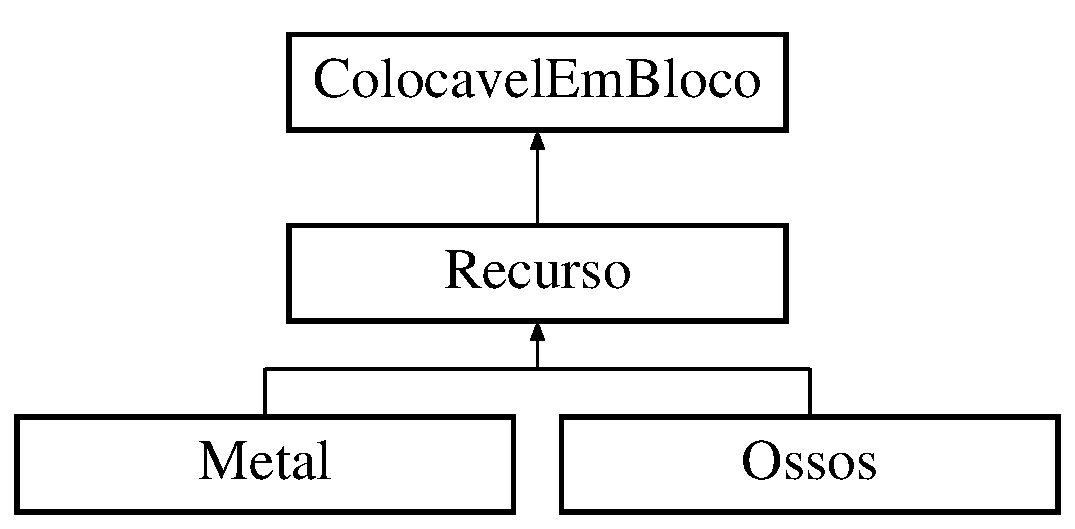
\includegraphics[height=3.000000cm]{class_recurso}
\end{center}
\end{figure}
\subsection*{Public Member Functions}
\begin{DoxyCompactItemize}
\item 
\mbox{\Hypertarget{class_recurso_a43cf1959ef600190ab7cdb74b9722d11}\label{class_recurso_a43cf1959ef600190ab7cdb74b9722d11}} 
\mbox{\hyperlink{class_recurso_a43cf1959ef600190ab7cdb74b9722d11}{Recurso}} ()
\begin{DoxyCompactList}\small\item\em Construct a new \mbox{\hyperlink{class_recurso}{Recurso}}\+:\+: \mbox{\hyperlink{class_recurso}{Recurso}} object. \end{DoxyCompactList}\end{DoxyCompactItemize}
\subsection*{Public Attributes}
\begin{DoxyCompactItemize}
\item 
\mbox{\Hypertarget{class_recurso_a270b8b705353deb293fdda57eb38d567}\label{class_recurso_a270b8b705353deb293fdda57eb38d567}} 
unsigned short {\bfseries qtde}
\item 
\mbox{\Hypertarget{class_recurso_a5a3d2e707dd3113235ab1132d0df77a3}\label{class_recurso_a5a3d2e707dd3113235ab1132d0df77a3}} 
Tipo\+Recurso {\bfseries tipo\+\_\+recurso}
\end{DoxyCompactItemize}


\subsection{Detailed Description}


Definition at line 27 of file Recurso.\+hpp.



The documentation for this class was generated from the following files\+:\begin{DoxyCompactItemize}
\item 
include/\mbox{\hyperlink{_recurso_8hpp}{Recurso.\+hpp}}\item 
src/\mbox{\hyperlink{_recurso_8cpp}{Recurso.\+cpp}}\end{DoxyCompactItemize}

\chapter{File Documentation}
\hypertarget{_bloco_8hpp}{}\section{include/\+Bloco.hpp File Reference}
\label{_bloco_8hpp}\index{include/\+Bloco.\+hpp@{include/\+Bloco.\+hpp}}
{\ttfamily \#include \char`\"{}Utils.\+hpp\char`\"{}}\newline
\subsection*{Classes}
\begin{DoxyCompactItemize}
\item 
class \mbox{\hyperlink{class_colocavel_em_bloco}{Colocavel\+Em\+Bloco}}
\item 
class \mbox{\hyperlink{class_bloco}{Bloco}}
\end{DoxyCompactItemize}
\subsection*{Enumerations}
\begin{DoxyCompactItemize}
\item 
\mbox{\Hypertarget{_bloco_8hpp_aa1d8b7a8ad4f7e5ef6b3641d87929624}\label{_bloco_8hpp_aa1d8b7a8ad4f7e5ef6b3641d87929624}} 
enum {\bfseries Tipo\+Conteudo\+Bloco} \{ {\bfseries U\+N\+I\+D\+A\+DE} = 0, 
{\bfseries P\+R\+E\+D\+IO}, 
{\bfseries R\+E\+C\+U\+R\+SO}
 \}
\end{DoxyCompactItemize}


\subsection{Detailed Description}
\begin{DoxyAuthor}{Author}
Alex Siqueira (\href{mailto:siqueiralex@github.com}{\tt siqueiralex@github.\+com}) 

Alexander André (\href{mailto:Alexander-1995@github.com}{\tt Alexander-\/1995@github.\+com}) 

Arthur Veiga (\href{mailto:arthurveiga@github.com}{\tt arthurveiga@github.\+com}) 

Matheus Veleci (\href{mailto:matheusvsantos@github.com}{\tt matheusvsantos@github.\+com}) 

Luis Luz (\href{mailto:lightguy875@github.com}{\tt lightguy875@github.\+com}) 
\end{DoxyAuthor}
\begin{DoxyVersion}{Version}
0.\+1 
\end{DoxyVersion}
\begin{DoxyDate}{Date}
2018-\/12-\/01
\end{DoxyDate}
\begin{DoxyCopyright}{Copyright}
Copyright (c) 2018 
\end{DoxyCopyright}

\hypertarget{_button_8hpp}{}\section{include/\+Button.hpp File Reference}
\label{_button_8hpp}\index{include/\+Button.\+hpp@{include/\+Button.\+hpp}}
{\ttfamily \#include \char`\"{}Game.\+hpp\char`\"{}}\newline
{\ttfamily \#include \char`\"{}common.\+hpp\char`\"{}}\newline
\subsection*{Classes}
\begin{DoxyCompactItemize}
\item 
class \mbox{\hyperlink{class_button}{Button}}
\end{DoxyCompactItemize}
\subsection*{Macros}
\begin{DoxyCompactItemize}
\item 
\mbox{\Hypertarget{_button_8hpp_aa87aa947426ab247561c8dbdb0e2bcf1}\label{_button_8hpp_aa87aa947426ab247561c8dbdb0e2bcf1}} 
\#define {\bfseries Button\+\_\+\+S\+T\+R\+U\+C\+T\+U\+RE}
\item 
\mbox{\Hypertarget{_button_8hpp_a579fab149208c817412ac02f0b21647d}\label{_button_8hpp_a579fab149208c817412ac02f0b21647d}} 
\#define {\bfseries T\+O\+T\+A\+L\+\_\+\+M\+E\+N\+U\+\_\+\+B\+U\+T\+T\+O\+NS}~3
\end{DoxyCompactItemize}
\subsection*{Enumerations}
\begin{DoxyCompactItemize}
\item 
\mbox{\Hypertarget{_button_8hpp_ae2d5c50fae96a83cc4f5974af78e6943}\label{_button_8hpp_ae2d5c50fae96a83cc4f5974af78e6943}} 
enum {\bfseries Button\+Type} \{ \newline
{\bfseries B\+U\+T\+T\+O\+N\+\_\+\+P\+L\+AY}, 
{\bfseries B\+U\+T\+T\+O\+N\+\_\+\+C\+R\+E\+D\+I\+TS}, 
{\bfseries B\+U\+T\+T\+O\+N\+\_\+\+Q\+U\+IT}, 
{\bfseries B\+U\+T\+T\+O\+N\+\_\+\+B\+A\+C\+K\+\_\+\+C\+R\+E\+D\+I\+TS}, 
\newline
{\bfseries B\+U\+T\+T\+O\+N\+\_\+\+B\+A\+C\+K\+\_\+\+G\+A\+ME}, 
{\bfseries B\+U\+T\+T\+O\+N\+\_\+\+C\+R\+I\+A\+R\+\_\+\+P\+I\+L\+A\+R\+\_\+\+A\+R\+CO}, 
{\bfseries B\+U\+T\+T\+O\+N\+\_\+\+C\+R\+I\+A\+R\+\_\+\+P\+I\+L\+A\+R\+\_\+\+L\+A\+N\+CA}, 
{\bfseries B\+U\+T\+T\+O\+N\+\_\+\+C\+R\+I\+A\+R\+\_\+\+P\+I\+L\+A\+R\+\_\+\+E\+S\+P\+A\+DA}, 
\newline
{\bfseries B\+U\+T\+T\+O\+N\+\_\+\+C\+R\+I\+A\+R\+\_\+\+N\+E\+C\+RO}, 
{\bfseries B\+U\+T\+T\+O\+N\+\_\+\+F\+O\+R\+T\+\_\+\+P\+I\+L\+AR}, 
{\bfseries B\+U\+T\+T\+O\+N\+\_\+\+F\+O\+R\+T\+\_\+\+N\+E\+C\+RO}, 
{\bfseries B\+U\+T\+T\+O\+N\+\_\+\+C\+R\+I\+AR}, 
\newline
{\bfseries C\+A\+N\+C\+EL}
 \}
\end{DoxyCompactItemize}


\subsection{Detailed Description}
\begin{DoxyAuthor}{Author}
Alex Siqueira (\href{mailto:siqueiralex@github.com}{\tt siqueiralex@github.\+com}) 

Alexander André (\href{mailto:Alexander-1995@github.com}{\tt Alexander-\/1995@github.\+com}) 

Arthur Veiga (\href{mailto:arthurveiga@github.com}{\tt arthurveiga@github.\+com}) 

Matheus Veleci (\href{mailto:matheusvsantos@github.com}{\tt matheusvsantos@github.\+com}) 

Luis Luz (\href{mailto:lightguy875@github.com}{\tt lightguy875@github.\+com}) 
\end{DoxyAuthor}
\begin{DoxyVersion}{Version}
0.\+1 
\end{DoxyVersion}
\begin{DoxyDate}{Date}
2018-\/12-\/01
\end{DoxyDate}
\begin{DoxyCopyright}{Copyright}
Copyright (c) 2018 
\end{DoxyCopyright}

\hypertarget{common_8hpp}{}\section{include/common.hpp File Reference}
\label{common_8hpp}\index{include/common.\+hpp@{include/common.\+hpp}}
{\ttfamily \#include \char`\"{}Button.\+hpp\char`\"{}}\newline
{\ttfamily \#include \char`\"{}Texture.\+hpp\char`\"{}}\newline
{\ttfamily \#include $<$S\+D\+L2/\+S\+D\+L\+\_\+ttf.\+h$>$}\newline
\subsection*{Macros}
\begin{DoxyCompactItemize}
\item 
\mbox{\Hypertarget{common_8hpp_a2cd109632a6dcccaa80b43561b1ab700}\label{common_8hpp_a2cd109632a6dcccaa80b43561b1ab700}} 
\#define {\bfseries S\+C\+R\+E\+E\+N\+\_\+\+W\+I\+D\+TH}~800
\item 
\mbox{\Hypertarget{common_8hpp_a6974d08a74da681b3957b2fead2608b8}\label{common_8hpp_a6974d08a74da681b3957b2fead2608b8}} 
\#define {\bfseries S\+C\+R\+E\+E\+N\+\_\+\+H\+E\+I\+G\+HT}~600
\item 
\mbox{\Hypertarget{common_8hpp_aa465c0206c08c9cde6075c2afb1c8bc8}\label{common_8hpp_aa465c0206c08c9cde6075c2afb1c8bc8}} 
\#define {\bfseries S\+Q\+U\+A\+R\+E\+\_\+\+S\+I\+ZE}~40
\item 
\mbox{\Hypertarget{common_8hpp_a4923a7390726728990e9fc9974658873}\label{common_8hpp_a4923a7390726728990e9fc9974658873}} 
\#define {\bfseries P\+L\+A\+Y\+E\+R\+\_\+\+A\+R\+E\+A\+\_\+\+S\+T\+A\+R\+T\+\_\+Y}~40
\item 
\mbox{\Hypertarget{common_8hpp_adaddb73885160218e7976e16815fd92e}\label{common_8hpp_adaddb73885160218e7976e16815fd92e}} 
\#define {\bfseries P\+L\+A\+Y\+E\+R\+\_\+\+A\+R\+E\+A\+\_\+\+E\+N\+D\+\_\+Y}~560
\item 
\mbox{\Hypertarget{common_8hpp_afe49ac6d27651b1b163c2ab258a3bb7c}\label{common_8hpp_afe49ac6d27651b1b163c2ab258a3bb7c}} 
\#define {\bfseries P\+L\+A\+Y\+E\+R\+\_\+\+A\+R\+E\+A\+\_\+\+S\+T\+A\+R\+T\+\_\+X}~120
\item 
\mbox{\Hypertarget{common_8hpp_aabe53f638533941e255c4d06e545e897}\label{common_8hpp_aabe53f638533941e255c4d06e545e897}} 
\#define {\bfseries P\+L\+A\+Y\+E\+R\+\_\+\+A\+R\+E\+A\+\_\+\+E\+N\+D\+\_\+X}~680
\end{DoxyCompactItemize}
\subsection*{Variables}
\begin{DoxyCompactItemize}
\item 
\mbox{\Hypertarget{common_8hpp_a918b230e9805d25f5fa32459a87dee8f}\label{common_8hpp_a918b230e9805d25f5fa32459a87dee8f}} 
\mbox{\hyperlink{class_button}{Button}} {\bfseries menu\+Buttons} \mbox{[}T\+O\+T\+A\+L\+\_\+\+M\+E\+N\+U\+\_\+\+B\+U\+T\+T\+O\+NS\mbox{]}
\item 
\mbox{\Hypertarget{common_8hpp_a4822d5e4e7fb2d26aedcd492c4254b7a}\label{common_8hpp_a4822d5e4e7fb2d26aedcd492c4254b7a}} 
\mbox{\hyperlink{class_button}{Button}} {\bfseries pause\+Button} \mbox{[}2\mbox{]}
\item 
\mbox{\Hypertarget{common_8hpp_a831bd72f9c6ffcc476f0df35eb411c59}\label{common_8hpp_a831bd72f9c6ffcc476f0df35eb411c59}} 
\mbox{\hyperlink{class_button}{Button}} {\bfseries credits\+Back\+Button}
\item 
\mbox{\Hypertarget{common_8hpp_aaa8e409e04dcf575ef63fd5fb3db06f9}\label{common_8hpp_aaa8e409e04dcf575ef63fd5fb3db06f9}} 
S\+D\+L\+\_\+\+Window $\ast$ {\bfseries window}
\item 
\mbox{\Hypertarget{common_8hpp_a966da7a60c4ea3ba301e26ccc5efe452}\label{common_8hpp_a966da7a60c4ea3ba301e26ccc5efe452}} 
S\+D\+L\+\_\+\+Renderer $\ast$ {\bfseries renderer}
\item 
\mbox{\Hypertarget{common_8hpp_a88e92429d5c1319c5a693c5e96742577}\label{common_8hpp_a88e92429d5c1319c5a693c5e96742577}} 
Texture {\bfseries menu\+\_\+screen}
\item 
\mbox{\Hypertarget{common_8hpp_a94bbf2b4f079b7abf8b8366267c1819d}\label{common_8hpp_a94bbf2b4f079b7abf8b8366267c1819d}} 
Texture {\bfseries credit\+\_\+screen}
\item 
\mbox{\Hypertarget{common_8hpp_a0c83ba420981799044096f0e61cd6130}\label{common_8hpp_a0c83ba420981799044096f0e61cd6130}} 
Texture {\bfseries pause\+\_\+screen}
\item 
\mbox{\Hypertarget{common_8hpp_a9d17e3b3d95f2f3bdfbb390349657f60}\label{common_8hpp_a9d17e3b3d95f2f3bdfbb390349657f60}} 
Texture {\bfseries round\+\_\+screen}
\item 
\mbox{\Hypertarget{common_8hpp_a5cd840b1b5ad682981b7aefc8c37b8c8}\label{common_8hpp_a5cd840b1b5ad682981b7aefc8c37b8c8}} 
Texture {\bfseries knight} \mbox{[}2\mbox{]}
\item 
\mbox{\Hypertarget{common_8hpp_afb0456214bf86e8255efbf93843e9c5b}\label{common_8hpp_afb0456214bf86e8255efbf93843e9c5b}} 
Texture {\bfseries solider} \mbox{[}2\mbox{]}
\item 
\mbox{\Hypertarget{common_8hpp_ace74383427c40e9917c56fad4b6f2c11}\label{common_8hpp_ace74383427c40e9917c56fad4b6f2c11}} 
Texture {\bfseries archer} \mbox{[}2\mbox{]}
\item 
\mbox{\Hypertarget{common_8hpp_ae4632d4c0660c7d35d3b86057bd7c2e9}\label{common_8hpp_ae4632d4c0660c7d35d3b86057bd7c2e9}} 
Texture {\bfseries map\+\_\+screen}
\item 
\mbox{\Hypertarget{common_8hpp_a10392e450938c1c3db72f902ebe36f7a}\label{common_8hpp_a10392e450938c1c3db72f902ebe36f7a}} 
Texture {\bfseries ganhou\+\_\+screen} \mbox{[}2\mbox{]}
\item 
\mbox{\Hypertarget{common_8hpp_abf5bfa705e66ffc1ddaa6ce46c960873}\label{common_8hpp_abf5bfa705e66ffc1ddaa6ce46c960873}} 
T\+T\+F\+\_\+\+Font $\ast$ {\bfseries font}
\item 
\mbox{\Hypertarget{common_8hpp_adb557ab7cf5ea08e8b024b64ae7fbbf7}\label{common_8hpp_adb557ab7cf5ea08e8b024b64ae7fbbf7}} 
Texture {\bfseries text\+Active\+Item}
\item 
\mbox{\Hypertarget{common_8hpp_a325d4592837174021a9691937f662dba}\label{common_8hpp_a325d4592837174021a9691937f662dba}} 
Texture {\bfseries text\+HP}
\item 
\mbox{\Hypertarget{common_8hpp_a993543549b5395e9004ca567bab1b997}\label{common_8hpp_a993543549b5395e9004ca567bab1b997}} 
Texture {\bfseries text\+Bones}
\item 
\mbox{\Hypertarget{common_8hpp_a595b1c1034a23eae04587313da684bbf}\label{common_8hpp_a595b1c1034a23eae04587313da684bbf}} 
Texture {\bfseries text\+Metal}
\item 
\mbox{\Hypertarget{common_8hpp_a5fdf598ed1ee9a242523b50687251e00}\label{common_8hpp_a5fdf598ed1ee9a242523b50687251e00}} 
Texture {\bfseries text\+Round}
\item 
\mbox{\Hypertarget{common_8hpp_a317243d7664c329128a0f4b6444a3c9b}\label{common_8hpp_a317243d7664c329128a0f4b6444a3c9b}} 
Texture {\bfseries pilar\+\_\+archer} \mbox{[}2\mbox{]}
\item 
\mbox{\Hypertarget{common_8hpp_a95dc3fcb509a2e27395399748755954b}\label{common_8hpp_a95dc3fcb509a2e27395399748755954b}} 
Texture {\bfseries pilar\+\_\+knight} \mbox{[}2\mbox{]}
\item 
\mbox{\Hypertarget{common_8hpp_a44877f53171b123e5ac2af041fe28ff7}\label{common_8hpp_a44877f53171b123e5ac2af041fe28ff7}} 
Texture {\bfseries pilar\+\_\+solider} \mbox{[}2\mbox{]}
\item 
\mbox{\Hypertarget{common_8hpp_ad1db82157cd98f00d6e7f9ef9b5637ad}\label{common_8hpp_ad1db82157cd98f00d6e7f9ef9b5637ad}} 
Texture {\bfseries bones} \mbox{[}20\mbox{]}
\item 
\mbox{\Hypertarget{common_8hpp_a712aa1c199e50ae301e38e36a62c2b4e}\label{common_8hpp_a712aa1c199e50ae301e38e36a62c2b4e}} 
Texture {\bfseries metal} \mbox{[}20\mbox{]}
\item 
\mbox{\Hypertarget{common_8hpp_abee26a5db07835674de8945f1227df02}\label{common_8hpp_abee26a5db07835674de8945f1227df02}} 
int {\bfseries ativo\+\_\+x\+\_\+jog}
\item 
\mbox{\Hypertarget{common_8hpp_af8b1c421c2b3f3474f60f3172232582c}\label{common_8hpp_af8b1c421c2b3f3474f60f3172232582c}} 
int {\bfseries ativo\+\_\+y\+\_\+jog}
\item 
\mbox{\Hypertarget{common_8hpp_a3af4fd2e68b24f6267ca0fdba135ce97}\label{common_8hpp_a3af4fd2e68b24f6267ca0fdba135ce97}} 
int {\bfseries ativo\+\_\+x\+\_\+cpu}
\item 
\mbox{\Hypertarget{common_8hpp_a5a03c7b0c242cb206996d29c58200e78}\label{common_8hpp_a5a03c7b0c242cb206996d29c58200e78}} 
int {\bfseries ativo\+\_\+y\+\_\+cpu}
\item 
\mbox{\Hypertarget{common_8hpp_ae8e5ca4ec014caadce25d80a7ec32912}\label{common_8hpp_ae8e5ca4ec014caadce25d80a7ec32912}} 
int {\bfseries ganhou\+\_\+time}
\end{DoxyCompactItemize}


\subsection{Detailed Description}
\begin{DoxyAuthor}{Author}
Alex Siqueira (\href{mailto:siqueiralex@github.com}{\tt siqueiralex@github.\+com}) 

Alexander André (\href{mailto:Alexander-1995@github.com}{\tt Alexander-\/1995@github.\+com}) 

Arthur Veiga (\href{mailto:arthurveiga@github.com}{\tt arthurveiga@github.\+com}) 

Matheus Veleci (\href{mailto:matheusvsantos@github.com}{\tt matheusvsantos@github.\+com}) 

Luis Luz (\href{mailto:lightguy875@github.com}{\tt lightguy875@github.\+com}) 
\end{DoxyAuthor}
\begin{DoxyVersion}{Version}
0.\+1 
\end{DoxyVersion}
\begin{DoxyDate}{Date}
2018-\/12-\/01
\end{DoxyDate}
\begin{DoxyCopyright}{Copyright}
Copyright (c) 2018 
\end{DoxyCopyright}

\hypertarget{_controlador_8hpp}{}\section{include/\+Controlador.hpp File Reference}
\label{_controlador_8hpp}\index{include/\+Controlador.\+hpp@{include/\+Controlador.\+hpp}}
{\ttfamily \#include $<$string$>$}\newline
{\ttfamily \#include $<$list$>$}\newline
{\ttfamily \#include $<$cmath$>$}\newline
{\ttfamily \#include \char`\"{}Recurso.\+hpp\char`\"{}}\newline
{\ttfamily \#include \char`\"{}Mapa.\+hpp\char`\"{}}\newline
{\ttfamily \#include \char`\"{}Player.\+hpp\char`\"{}}\newline
{\ttfamily \#include \char`\"{}Utils.\+hpp\char`\"{}}\newline
\subsection*{Classes}
\begin{DoxyCompactItemize}
\item 
class \mbox{\hyperlink{class_controlador}{Controlador}}
\end{DoxyCompactItemize}


\subsection{Detailed Description}
\begin{DoxyAuthor}{Author}
Alex Siqueira (\href{mailto:siqueiralex@github.com}{\tt siqueiralex@github.\+com}) 

Alexander André (\href{mailto:Alexander-1995@github.com}{\tt Alexander-\/1995@github.\+com}) 

Arthur Veiga (\href{mailto:arthurveiga@github.com}{\tt arthurveiga@github.\+com}) 

Matheus Veleci (\href{mailto:matheusvsantos@github.com}{\tt matheusvsantos@github.\+com}) 

Luis Luz (\href{mailto:lightguy875@github.com}{\tt lightguy875@github.\+com}) 
\end{DoxyAuthor}
\begin{DoxyVersion}{Version}
0.\+1 
\end{DoxyVersion}
\begin{DoxyDate}{Date}
2018-\/12-\/01
\end{DoxyDate}
\begin{DoxyCopyright}{Copyright}
Copyright (c) 2018 
\end{DoxyCopyright}

\hypertarget{_game_8hpp}{}\section{include/\+Game.hpp File Reference}
\label{_game_8hpp}\index{include/\+Game.\+hpp@{include/\+Game.\+hpp}}
{\ttfamily \#include \char`\"{}common.\+hpp\char`\"{}}\newline
{\ttfamily \#include $<$S\+D\+L2/\+S\+D\+L\+\_\+image.\+h$>$}\newline
{\ttfamily \#include $<$S\+D\+L2/\+S\+D\+L.\+h$>$}\newline


\subsection{Detailed Description}
\begin{DoxyAuthor}{Author}
Alex Siqueira (\href{mailto:siqueiralex@github.com}{\tt siqueiralex@github.\+com}) 

Alexander André (\href{mailto:Alexander-1995@github.com}{\tt Alexander-\/1995@github.\+com}) 

Arthur Veiga (\href{mailto:arthurveiga@github.com}{\tt arthurveiga@github.\+com}) 

Matheus Veleci (\href{mailto:matheusvsantos@github.com}{\tt matheusvsantos@github.\+com}) 

Luis Luz (\href{mailto:lightguy875@github.com}{\tt lightguy875@github.\+com}) 
\end{DoxyAuthor}
\begin{DoxyVersion}{Version}
0.\+1 
\end{DoxyVersion}
\begin{DoxyDate}{Date}
2018-\/12-\/01
\end{DoxyDate}
\begin{DoxyCopyright}{Copyright}
Copyright (c) 2018 
\end{DoxyCopyright}

\hypertarget{_graphics_8hpp}{}\section{include/\+Graphics.hpp File Reference}
\label{_graphics_8hpp}\index{include/\+Graphics.\+hpp@{include/\+Graphics.\+hpp}}
{\ttfamily \#include $<$S\+D\+L2/\+S\+D\+L\+\_\+image.\+h$>$}\newline
{\ttfamily \#include $<$S\+D\+L2/\+S\+D\+L.\+h$>$}\newline
{\ttfamily \#include $<$S\+D\+L2/\+S\+D\+L\+\_\+ttf.\+h$>$}\newline
{\ttfamily \#include \char`\"{}Texture.\+hpp\char`\"{}}\newline
{\ttfamily \#include \char`\"{}common.\+hpp\char`\"{}}\newline
\subsection*{Classes}
\begin{DoxyCompactItemize}
\item 
class \mbox{\hyperlink{class_graphics}{Graphics}}
\end{DoxyCompactItemize}


\subsection{Detailed Description}
\begin{DoxyAuthor}{Author}
Alex Siqueira (\href{mailto:siqueiralex@github.com}{\tt siqueiralex@github.\+com}) 

Alexander André (\href{mailto:Alexander-1995@github.com}{\tt Alexander-\/1995@github.\+com}) 

Arthur Veiga (\href{mailto:arthurveiga@github.com}{\tt arthurveiga@github.\+com}) 

Matheus Veleci (\href{mailto:matheusvsantos@github.com}{\tt matheusvsantos@github.\+com}) 

Luis Luz (\href{mailto:lightguy875@github.com}{\tt lightguy875@github.\+com}) 
\end{DoxyAuthor}
\begin{DoxyVersion}{Version}
0.\+1 
\end{DoxyVersion}
\begin{DoxyDate}{Date}
2018-\/12-\/01
\end{DoxyDate}
\begin{DoxyCopyright}{Copyright}
Copyright (c) 2018 
\end{DoxyCopyright}

\hypertarget{_mapa_8hpp}{}\section{include/\+Mapa.hpp File Reference}
\label{_mapa_8hpp}\index{include/\+Mapa.\+hpp@{include/\+Mapa.\+hpp}}
{\ttfamily \#include $<$tuple$>$}\newline
{\ttfamily \#include $<$map$>$}\newline
{\ttfamily \#include \char`\"{}Bloco.\+hpp\char`\"{}}\newline
\subsection*{Classes}
\begin{DoxyCompactItemize}
\item 
class \mbox{\hyperlink{class_mapa}{Mapa}}
\end{DoxyCompactItemize}
\subsection*{Typedefs}
\begin{DoxyCompactItemize}
\item 
\mbox{\Hypertarget{_mapa_8hpp_a84537d48098426a5ca151c8e9a9998d0}\label{_mapa_8hpp_a84537d48098426a5ca151c8e9a9998d0}} 
typedef std\+::pair$<$ unsigned short, unsigned short $>$ {\bfseries Posicao}
\item 
\mbox{\Hypertarget{_mapa_8hpp_a277824eeb3f9d9af719abc5f8aa89dfb}\label{_mapa_8hpp_a277824eeb3f9d9af719abc5f8aa89dfb}} 
typedef std\+::map$<$ Posicao, \mbox{\hyperlink{class_bloco}{Bloco}} $>$ {\bfseries Mapa\+De\+Blocos}
\end{DoxyCompactItemize}


\subsection{Detailed Description}
\begin{DoxyAuthor}{Author}
Alex Siqueira (\href{mailto:siqueiralex@github.com}{\tt siqueiralex@github.\+com}) 

Alexander André (\href{mailto:Alexander-1995@github.com}{\tt Alexander-\/1995@github.\+com}) 

Arthur Veiga (\href{mailto:arthurveiga@github.com}{\tt arthurveiga@github.\+com}) 

Matheus Veleci (\href{mailto:matheusvsantos@github.com}{\tt matheusvsantos@github.\+com}) 

Luis Luz (\href{mailto:lightguy875@github.com}{\tt lightguy875@github.\+com}) 
\end{DoxyAuthor}
\begin{DoxyVersion}{Version}
0.\+1 
\end{DoxyVersion}
\begin{DoxyDate}{Date}
2018-\/12-\/01
\end{DoxyDate}
\begin{DoxyCopyright}{Copyright}
Copyright (c) 2018 
\end{DoxyCopyright}

\hypertarget{_necromancer_8hpp}{}\section{include/\+Necromancer.hpp File Reference}
\label{_necromancer_8hpp}\index{include/\+Necromancer.\+hpp@{include/\+Necromancer.\+hpp}}
{\ttfamily \#include $<$S\+D\+L2/\+S\+D\+L\+\_\+image.\+h$>$}\newline
{\ttfamily \#include $<$S\+D\+L2/\+S\+D\+L.\+h$>$}\newline
{\ttfamily \#include \char`\"{}Bloco.\+hpp\char`\"{}}\newline
{\ttfamily \#include \char`\"{}Pilar.\+hpp\char`\"{}}\newline
{\ttfamily \#include \char`\"{}Utils.\+hpp\char`\"{}}\newline
\subsection*{Classes}
\begin{DoxyCompactItemize}
\item 
class \mbox{\hyperlink{class_necromancer}{Necromancer}}
\item 
class \mbox{\hyperlink{class_guerreiro}{Guerreiro}}
\item 
class \mbox{\hyperlink{class_cavaleiro}{Cavaleiro}}
\item 
class \mbox{\hyperlink{class_arqueiro}{Arqueiro}}
\end{DoxyCompactItemize}
\subsection*{Enumerations}
\begin{DoxyCompactItemize}
\item 
\mbox{\Hypertarget{_necromancer_8hpp_ac3271bec28560054d3c581c9f7ba162e}\label{_necromancer_8hpp_ac3271bec28560054d3c581c9f7ba162e}} 
enum {\bfseries Tipo\+Necromancer} \{ {\bfseries G\+U\+E\+R\+R\+E\+I\+RO} = 4, 
{\bfseries C\+A\+V\+A\+L\+E\+I\+RO}, 
{\bfseries A\+R\+Q\+U\+E\+I\+RO}
 \}
\end{DoxyCompactItemize}


\subsection{Detailed Description}
\begin{DoxyAuthor}{Author}
Alex Siqueira (\href{mailto:siqueiralex@github.com}{\tt siqueiralex@github.\+com}) 

Alexander André (\href{mailto:Alexander-1995@github.com}{\tt Alexander-\/1995@github.\+com}) 

Arthur Veiga (\href{mailto:arthurveiga@github.com}{\tt arthurveiga@github.\+com}) 

Matheus Veleci (\href{mailto:matheusvsantos@github.com}{\tt matheusvsantos@github.\+com}) 

Luis Luz (\href{mailto:lightguy875@github.com}{\tt lightguy875@github.\+com}) 
\end{DoxyAuthor}
\begin{DoxyVersion}{Version}
0.\+1 
\end{DoxyVersion}
\begin{DoxyDate}{Date}
2018-\/12-\/01
\end{DoxyDate}
\begin{DoxyCopyright}{Copyright}
Copyright (c) 2018 
\end{DoxyCopyright}

\hypertarget{_pilar_8hpp}{}\section{include/\+Pilar.hpp File Reference}
\label{_pilar_8hpp}\index{include/\+Pilar.\+hpp@{include/\+Pilar.\+hpp}}
{\ttfamily \#include \char`\"{}Bloco.\+hpp\char`\"{}}\newline
{\ttfamily \#include \char`\"{}Utils.\+hpp\char`\"{}}\newline
{\ttfamily \#include \char`\"{}common.\+hpp\char`\"{}}\newline
\subsection*{Classes}
\begin{DoxyCompactItemize}
\item 
class \mbox{\hyperlink{class_pilar}{Pilar}}
\item 
class \mbox{\hyperlink{class_pilar_espada}{Pilar\+Espada}}
\item 
class \mbox{\hyperlink{class_pilar_lanca}{Pilar\+Lanca}}
\item 
class \mbox{\hyperlink{class_pilar_arco}{Pilar\+Arco}}
\end{DoxyCompactItemize}
\subsection*{Enumerations}
\begin{DoxyCompactItemize}
\item 
\mbox{\Hypertarget{_pilar_8hpp_ab97739e93f1d75b9711fef5b6237e66b}\label{_pilar_8hpp_ab97739e93f1d75b9711fef5b6237e66b}} 
enum {\bfseries Tipo\+Pilar} \{ {\bfseries E\+S\+P\+A\+DA} = 7, 
{\bfseries L\+A\+N\+CA}, 
{\bfseries A\+R\+CO}
 \}
\end{DoxyCompactItemize}


\subsection{Detailed Description}
\begin{DoxyAuthor}{Author}
Alex Siqueira (\href{mailto:siqueiralex@github.com}{\tt siqueiralex@github.\+com}) 

Alexander André (\href{mailto:Alexander-1995@github.com}{\tt Alexander-\/1995@github.\+com}) 

Arthur Veiga (\href{mailto:arthurveiga@github.com}{\tt arthurveiga@github.\+com}) 

Matheus Veleci (\href{mailto:matheusvsantos@github.com}{\tt matheusvsantos@github.\+com}) 

Luis Luz (\href{mailto:lightguy875@github.com}{\tt lightguy875@github.\+com}) 
\end{DoxyAuthor}
\begin{DoxyVersion}{Version}
0.\+1 
\end{DoxyVersion}
\begin{DoxyDate}{Date}
2018-\/12-\/01
\end{DoxyDate}
\begin{DoxyCopyright}{Copyright}
Copyright (c) 2018 
\end{DoxyCopyright}

\hypertarget{_player_8hpp}{}\section{include/\+Player.hpp File Reference}
\label{_player_8hpp}\index{include/\+Player.\+hpp@{include/\+Player.\+hpp}}
{\ttfamily \#include \char`\"{}Necromancer.\+hpp\char`\"{}}\newline
{\ttfamily \#include \char`\"{}Pilar.\+hpp\char`\"{}}\newline
{\ttfamily \#include \char`\"{}Recurso.\+hpp\char`\"{}}\newline
{\ttfamily \#include \char`\"{}Utils.\+hpp\char`\"{}}\newline
\subsection*{Classes}
\begin{DoxyCompactItemize}
\item 
class \mbox{\hyperlink{class_player}{Player}}
\end{DoxyCompactItemize}


\subsection{Detailed Description}
\begin{DoxyAuthor}{Author}
Alex Siqueira (\href{mailto:siqueiralex@github.com}{\tt siqueiralex@github.\+com}) 

Alexander André (\href{mailto:Alexander-1995@github.com}{\tt Alexander-\/1995@github.\+com}) 

Arthur Veiga (\href{mailto:arthurveiga@github.com}{\tt arthurveiga@github.\+com}) 

Matheus Veleci (\href{mailto:matheusvsantos@github.com}{\tt matheusvsantos@github.\+com}) 

Luis Luz (\href{mailto:lightguy875@github.com}{\tt lightguy875@github.\+com}) 
\end{DoxyAuthor}
\begin{DoxyVersion}{Version}
0.\+1 
\end{DoxyVersion}
\begin{DoxyDate}{Date}
2018-\/12-\/01
\end{DoxyDate}
\begin{DoxyCopyright}{Copyright}
Copyright (c) 2018 
\end{DoxyCopyright}

\hypertarget{_recurso_8hpp}{}\section{include/\+Recurso.hpp File Reference}
\label{_recurso_8hpp}\index{include/\+Recurso.\+hpp@{include/\+Recurso.\+hpp}}
{\ttfamily \#include \char`\"{}Bloco.\+hpp\char`\"{}}\newline
{\ttfamily \#include \char`\"{}Utils.\+hpp\char`\"{}}\newline
\subsection*{Classes}
\begin{DoxyCompactItemize}
\item 
class \mbox{\hyperlink{class_recurso}{Recurso}}
\item 
class \mbox{\hyperlink{class_metal}{Metal}}
\item 
class \mbox{\hyperlink{class_ossos}{Ossos}}
\end{DoxyCompactItemize}
\subsection*{Enumerations}
\begin{DoxyCompactItemize}
\item 
\mbox{\Hypertarget{_recurso_8hpp_af185edab70d7be27bd991eec1b598791}\label{_recurso_8hpp_af185edab70d7be27bd991eec1b598791}} 
enum {\bfseries Tipo\+Recurso} \{ {\bfseries M\+E\+T\+AL} = 10, 
{\bfseries O\+S\+S\+OS}
 \}
\end{DoxyCompactItemize}


\subsection{Detailed Description}
\begin{DoxyAuthor}{Author}
Alex Siqueira (\href{mailto:siqueiralex@github.com}{\tt siqueiralex@github.\+com}) 

Alexander André (\href{mailto:Alexander-1995@github.com}{\tt Alexander-\/1995@github.\+com}) 

Arthur Veiga (\href{mailto:arthurveiga@github.com}{\tt arthurveiga@github.\+com}) 

Matheus Veleci (\href{mailto:matheusvsantos@github.com}{\tt matheusvsantos@github.\+com}) 

Luis Luz (\href{mailto:lightguy875@github.com}{\tt lightguy875@github.\+com}) 
\end{DoxyAuthor}
\begin{DoxyVersion}{Version}
0.\+1 
\end{DoxyVersion}
\begin{DoxyDate}{Date}
2018-\/12-\/01
\end{DoxyDate}
\begin{DoxyCopyright}{Copyright}
Copyright (c) 2018 
\end{DoxyCopyright}

\hypertarget{_texture_8hpp}{}\section{include/\+Texture.hpp File Reference}
\label{_texture_8hpp}\index{include/\+Texture.\+hpp@{include/\+Texture.\+hpp}}
{\ttfamily \#include $<$S\+D\+L2/\+S\+D\+L\+\_\+image.\+h$>$}\newline
{\ttfamily \#include $<$S\+D\+L2/\+S\+D\+L.\+h$>$}\newline
{\ttfamily \#include \char`\"{}common.\+hpp\char`\"{}}\newline
{\ttfamily \#include $<$string$>$}\newline


\subsection{Detailed Description}
\begin{DoxyAuthor}{Author}
Alex Siqueira (\href{mailto:siqueiralex@github.com}{\tt siqueiralex@github.\+com}) 

Alexander André (\href{mailto:Alexander-1995@github.com}{\tt Alexander-\/1995@github.\+com}) 

Arthur Veiga (\href{mailto:arthurveiga@github.com}{\tt arthurveiga@github.\+com}) 

Matheus Veleci (\href{mailto:matheusvsantos@github.com}{\tt matheusvsantos@github.\+com}) 

Luis Luz (\href{mailto:lightguy875@github.com}{\tt lightguy875@github.\+com}) 
\end{DoxyAuthor}
\begin{DoxyVersion}{Version}
0.\+1 
\end{DoxyVersion}
\begin{DoxyDate}{Date}
2018-\/12-\/01
\end{DoxyDate}
\begin{DoxyCopyright}{Copyright}
Copyright (c) 2018 
\end{DoxyCopyright}

\hypertarget{_bloco_8cpp}{}\section{src/\+Bloco.cpp File Reference}
\label{_bloco_8cpp}\index{src/\+Bloco.\+cpp@{src/\+Bloco.\+cpp}}
{\ttfamily \#include \char`\"{}../include/\+Bloco.\+hpp\char`\"{}}\newline
{\ttfamily \#include $<$iostream$>$}\newline


\subsection{Detailed Description}
\begin{DoxyAuthor}{Author}
Alex Siqueira (\href{mailto:siqueiralex@github.com}{\tt siqueiralex@github.\+com}) 

Alexander André (\href{mailto:Alexander-1995@github.com}{\tt Alexander-\/1995@github.\+com}) 

Arthur Veiga (\href{mailto:arthurveiga@github.com}{\tt arthurveiga@github.\+com}) 

Matheus Veleci (\href{mailto:matheusvsantos@github.com}{\tt matheusvsantos@github.\+com}) 

Luis Luz (\href{mailto:lightguy875@github.com}{\tt lightguy875@github.\+com}) 
\end{DoxyAuthor}
\begin{DoxyDate}{Date}
2018-\/12-\/01
\end{DoxyDate}
\begin{DoxyCopyright}{Copyright}
Copyright (c) 2018 
\end{DoxyCopyright}

\hypertarget{_button_8cpp}{}\section{src/\+Button.cpp File Reference}
\label{_button_8cpp}\index{src/\+Button.\+cpp@{src/\+Button.\+cpp}}
{\ttfamily \#include \char`\"{}../include/\+Button.\+hpp\char`\"{}}\newline


\subsection{Detailed Description}
\begin{DoxyAuthor}{Author}
Alex Siqueira (\href{mailto:siqueiralex@github.com}{\tt siqueiralex@github.\+com}) 

Alexander André (\href{mailto:Alexander-1995@github.com}{\tt Alexander-\/1995@github.\+com}) 

Arthur Veiga (\href{mailto:arthurveiga@github.com}{\tt arthurveiga@github.\+com}) 

Matheus Veleci (\href{mailto:matheusvsantos@github.com}{\tt matheusvsantos@github.\+com}) 

Luis Luz (\href{mailto:lightguy875@github.com}{\tt lightguy875@github.\+com}) 
\end{DoxyAuthor}
\begin{DoxyVersion}{Version}
0.\+1 
\end{DoxyVersion}
\begin{DoxyDate}{Date}
2018-\/12-\/01
\end{DoxyDate}
\begin{DoxyCopyright}{Copyright}
Copyright (c) 2018 
\end{DoxyCopyright}

\hypertarget{_controlador_8cpp}{}\section{src/\+Controlador.cpp File Reference}
\label{_controlador_8cpp}\index{src/\+Controlador.\+cpp@{src/\+Controlador.\+cpp}}
{\ttfamily \#include $<$string$>$}\newline
{\ttfamily \#include $<$sstream$>$}\newline
{\ttfamily \#include $<$iostream$>$}\newline
{\ttfamily \#include \char`\"{}../include/\+Controlador.\+hpp\char`\"{}}\newline
{\ttfamily \#include \char`\"{}../include/common.\+hpp\char`\"{}}\newline


\subsection{Detailed Description}
\begin{DoxyAuthor}{Author}
Alex Siqueira (\href{mailto:siqueiralex@github.com}{\tt siqueiralex@github.\+com}) 

Alexander André (\href{mailto:Alexander-1995@github.com}{\tt Alexander-\/1995@github.\+com}) 

Arthur Veiga (\href{mailto:arthurveiga@github.com}{\tt arthurveiga@github.\+com}) 

Matheus Veleci (\href{mailto:matheusvsantos@github.com}{\tt matheusvsantos@github.\+com}) 

Luis Luz (\href{mailto:lightguy875@github.com}{\tt lightguy875@github.\+com}) 
\end{DoxyAuthor}
\begin{DoxyVersion}{Version}
0.\+1 
\end{DoxyVersion}
\begin{DoxyDate}{Date}
2018-\/12-\/01
\end{DoxyDate}
\begin{DoxyCopyright}{Copyright}
Copyright (c) 2018 
\end{DoxyCopyright}

\hypertarget{_game_8cpp}{}\section{src/\+Game.cpp File Reference}
\label{_game_8cpp}\index{src/\+Game.\+cpp@{src/\+Game.\+cpp}}
{\ttfamily \#include $<$cstdio$>$}\newline
{\ttfamily \#include $<$string$>$}\newline
{\ttfamily \#include $<$sstream$>$}\newline
{\ttfamily \#include \char`\"{}../include/\+Game.\+hpp\char`\"{}}\newline
{\ttfamily \#include \char`\"{}../include/\+Controlador.\+hpp\char`\"{}}\newline
\subsection*{Functions}
\begin{DoxyCompactItemize}
\item 
\mbox{\Hypertarget{_game_8cpp_a60a8733940eaa93946bcb88f95b0b3f8}\label{_game_8cpp_a60a8733940eaa93946bcb88f95b0b3f8}} 
void {\bfseries box\+Warning} (string text)
\item 
\mbox{\Hypertarget{_game_8cpp_abf5ea2496999acf32686492f8d9b1b3c}\label{_game_8cpp_abf5ea2496999acf32686492f8d9b1b3c}} 
void {\bfseries box\+Criar\+Pilar} (\mbox{\hyperlink{class_controlador}{Controlador}} $\ast$controlador)
\item 
\mbox{\Hypertarget{_game_8cpp_a369b86f311d7e2359352af84905ceda1}\label{_game_8cpp_a369b86f311d7e2359352af84905ceda1}} 
void {\bfseries box\+Criar\+Necro} (\mbox{\hyperlink{class_controlador}{Controlador}} $\ast$controlador, Tipo\+Pilar tipo\+\_\+p)
\item 
\mbox{\Hypertarget{_game_8cpp_a7840008bdd2f73d47fa9b1287e4c4f77}\label{_game_8cpp_a7840008bdd2f73d47fa9b1287e4c4f77}} 
int {\bfseries box\+Pilar} ()
\item 
\mbox{\Hypertarget{_game_8cpp_abec4eab92e9b46eb3d8e5cdbba03f58a}\label{_game_8cpp_abec4eab92e9b46eb3d8e5cdbba03f58a}} 
void {\bfseries action\+\_\+pilar\+\_\+option} (int option, \mbox{\hyperlink{class_controlador}{Controlador}} $\ast$controlador, Tipo\+Pilar tipo\+\_\+p, Tipo\+Necromancer tipo\+\_\+n)
\item 
\mbox{\Hypertarget{_game_8cpp_a0c80deb22cc64d0c2d8944e01212f026}\label{_game_8cpp_a0c80deb22cc64d0c2d8944e01212f026}} 
void {\bfseries handle\+\_\+necro\+\_\+ativo} (\mbox{\hyperlink{class_controlador}{Controlador}} $\ast$controlador, S\+D\+L\+\_\+\+Event $\ast$e, int i, int j)
\item 
\mbox{\Hypertarget{_game_8cpp_a0474f994efa2de8341a23085c319e21a}\label{_game_8cpp_a0474f994efa2de8341a23085c319e21a}} 
void {\bfseries handle\+\_\+events\+\_\+elements} (\mbox{\hyperlink{class_controlador}{Controlador}} $\ast$controlador, S\+D\+L\+\_\+\+Event $\ast$e)
\item 
\mbox{\Hypertarget{_game_8cpp_a42f778fefd313361854cfeecc293ee4d}\label{_game_8cpp_a42f778fefd313361854cfeecc293ee4d}} 
void {\bfseries movimentar\+\_\+ativo} (\mbox{\hyperlink{class_controlador}{Controlador}} $\ast$controlador, S\+D\+L\+\_\+\+Event $\ast$e)
\end{DoxyCompactItemize}


\subsection{Detailed Description}
\begin{DoxyAuthor}{Author}
Alex Siqueira (\href{mailto:siqueiralex@github.com}{\tt siqueiralex@github.\+com}) 

Alexander André (\href{mailto:Alexander-1995@github.com}{\tt Alexander-\/1995@github.\+com}) 

Arthur Veiga (\href{mailto:arthurveiga@github.com}{\tt arthurveiga@github.\+com}) 

Matheus Veleci (\href{mailto:matheusvsantos@github.com}{\tt matheusvsantos@github.\+com}) 

Luis Luz (\href{mailto:lightguy875@github.com}{\tt lightguy875@github.\+com}) 
\end{DoxyAuthor}
\begin{DoxyVersion}{Version}
0.\+1 
\end{DoxyVersion}
\begin{DoxyDate}{Date}
2018-\/12-\/01
\end{DoxyDate}
\begin{DoxyCopyright}{Copyright}
Copyright (c) 2018 
\end{DoxyCopyright}

\hypertarget{_graphics_8cpp}{}\section{src/\+Graphics.cpp File Reference}
\label{_graphics_8cpp}\index{src/\+Graphics.\+cpp@{src/\+Graphics.\+cpp}}
{\ttfamily \#include \char`\"{}../include/\+Graphics.\+hpp\char`\"{}}\newline
\subsection*{Variables}
\begin{DoxyCompactItemize}
\item 
\mbox{\Hypertarget{_graphics_8cpp_a918b230e9805d25f5fa32459a87dee8f}\label{_graphics_8cpp_a918b230e9805d25f5fa32459a87dee8f}} 
\mbox{\hyperlink{class_button}{Button}} {\bfseries menu\+Buttons} \mbox{[}T\+O\+T\+A\+L\+\_\+\+M\+E\+N\+U\+\_\+\+B\+U\+T\+T\+O\+NS\mbox{]}
\item 
\mbox{\Hypertarget{_graphics_8cpp_a4822d5e4e7fb2d26aedcd492c4254b7a}\label{_graphics_8cpp_a4822d5e4e7fb2d26aedcd492c4254b7a}} 
\mbox{\hyperlink{class_button}{Button}} {\bfseries pause\+Button} \mbox{[}2\mbox{]}
\item 
\mbox{\Hypertarget{_graphics_8cpp_a831bd72f9c6ffcc476f0df35eb411c59}\label{_graphics_8cpp_a831bd72f9c6ffcc476f0df35eb411c59}} 
\mbox{\hyperlink{class_button}{Button}} {\bfseries credits\+Back\+Button}
\item 
\mbox{\Hypertarget{_graphics_8cpp_aaa8e409e04dcf575ef63fd5fb3db06f9}\label{_graphics_8cpp_aaa8e409e04dcf575ef63fd5fb3db06f9}} 
S\+D\+L\+\_\+\+Window $\ast$ {\bfseries window} = N\+U\+LL
\item 
\mbox{\Hypertarget{_graphics_8cpp_a966da7a60c4ea3ba301e26ccc5efe452}\label{_graphics_8cpp_a966da7a60c4ea3ba301e26ccc5efe452}} 
S\+D\+L\+\_\+\+Renderer $\ast$ {\bfseries renderer} = N\+U\+LL
\item 
\mbox{\Hypertarget{_graphics_8cpp_a88e92429d5c1319c5a693c5e96742577}\label{_graphics_8cpp_a88e92429d5c1319c5a693c5e96742577}} 
Texture {\bfseries menu\+\_\+screen}
\item 
\mbox{\Hypertarget{_graphics_8cpp_a94bbf2b4f079b7abf8b8366267c1819d}\label{_graphics_8cpp_a94bbf2b4f079b7abf8b8366267c1819d}} 
Texture {\bfseries credit\+\_\+screen}
\item 
\mbox{\Hypertarget{_graphics_8cpp_a0c83ba420981799044096f0e61cd6130}\label{_graphics_8cpp_a0c83ba420981799044096f0e61cd6130}} 
Texture {\bfseries pause\+\_\+screen}
\item 
\mbox{\Hypertarget{_graphics_8cpp_a9d17e3b3d95f2f3bdfbb390349657f60}\label{_graphics_8cpp_a9d17e3b3d95f2f3bdfbb390349657f60}} 
Texture {\bfseries round\+\_\+screen}
\item 
\mbox{\Hypertarget{_graphics_8cpp_a5cd840b1b5ad682981b7aefc8c37b8c8}\label{_graphics_8cpp_a5cd840b1b5ad682981b7aefc8c37b8c8}} 
Texture {\bfseries knight} \mbox{[}2\mbox{]}
\item 
\mbox{\Hypertarget{_graphics_8cpp_afb0456214bf86e8255efbf93843e9c5b}\label{_graphics_8cpp_afb0456214bf86e8255efbf93843e9c5b}} 
Texture {\bfseries solider} \mbox{[}2\mbox{]}
\item 
\mbox{\Hypertarget{_graphics_8cpp_ace74383427c40e9917c56fad4b6f2c11}\label{_graphics_8cpp_ace74383427c40e9917c56fad4b6f2c11}} 
Texture {\bfseries archer} \mbox{[}2\mbox{]}
\item 
\mbox{\Hypertarget{_graphics_8cpp_ae4632d4c0660c7d35d3b86057bd7c2e9}\label{_graphics_8cpp_ae4632d4c0660c7d35d3b86057bd7c2e9}} 
Texture {\bfseries map\+\_\+screen}
\item 
\mbox{\Hypertarget{_graphics_8cpp_a10392e450938c1c3db72f902ebe36f7a}\label{_graphics_8cpp_a10392e450938c1c3db72f902ebe36f7a}} 
Texture {\bfseries ganhou\+\_\+screen} \mbox{[}2\mbox{]}
\item 
\mbox{\Hypertarget{_graphics_8cpp_abf5bfa705e66ffc1ddaa6ce46c960873}\label{_graphics_8cpp_abf5bfa705e66ffc1ddaa6ce46c960873}} 
T\+T\+F\+\_\+\+Font $\ast$ {\bfseries font}
\item 
\mbox{\Hypertarget{_graphics_8cpp_adb557ab7cf5ea08e8b024b64ae7fbbf7}\label{_graphics_8cpp_adb557ab7cf5ea08e8b024b64ae7fbbf7}} 
Texture {\bfseries text\+Active\+Item}
\item 
\mbox{\Hypertarget{_graphics_8cpp_a325d4592837174021a9691937f662dba}\label{_graphics_8cpp_a325d4592837174021a9691937f662dba}} 
Texture {\bfseries text\+HP}
\item 
\mbox{\Hypertarget{_graphics_8cpp_a993543549b5395e9004ca567bab1b997}\label{_graphics_8cpp_a993543549b5395e9004ca567bab1b997}} 
Texture {\bfseries text\+Bones}
\item 
\mbox{\Hypertarget{_graphics_8cpp_a595b1c1034a23eae04587313da684bbf}\label{_graphics_8cpp_a595b1c1034a23eae04587313da684bbf}} 
Texture {\bfseries text\+Metal}
\item 
\mbox{\Hypertarget{_graphics_8cpp_a5fdf598ed1ee9a242523b50687251e00}\label{_graphics_8cpp_a5fdf598ed1ee9a242523b50687251e00}} 
Texture {\bfseries text\+Round}
\item 
\mbox{\Hypertarget{_graphics_8cpp_a317243d7664c329128a0f4b6444a3c9b}\label{_graphics_8cpp_a317243d7664c329128a0f4b6444a3c9b}} 
Texture {\bfseries pilar\+\_\+archer} \mbox{[}2\mbox{]}
\item 
\mbox{\Hypertarget{_graphics_8cpp_a95dc3fcb509a2e27395399748755954b}\label{_graphics_8cpp_a95dc3fcb509a2e27395399748755954b}} 
Texture {\bfseries pilar\+\_\+knight} \mbox{[}2\mbox{]}
\item 
\mbox{\Hypertarget{_graphics_8cpp_a44877f53171b123e5ac2af041fe28ff7}\label{_graphics_8cpp_a44877f53171b123e5ac2af041fe28ff7}} 
Texture {\bfseries pilar\+\_\+solider} \mbox{[}2\mbox{]}
\item 
\mbox{\Hypertarget{_graphics_8cpp_ad1db82157cd98f00d6e7f9ef9b5637ad}\label{_graphics_8cpp_ad1db82157cd98f00d6e7f9ef9b5637ad}} 
Texture {\bfseries bones} \mbox{[}20\mbox{]}
\item 
\mbox{\Hypertarget{_graphics_8cpp_a712aa1c199e50ae301e38e36a62c2b4e}\label{_graphics_8cpp_a712aa1c199e50ae301e38e36a62c2b4e}} 
Texture {\bfseries metal} \mbox{[}20\mbox{]}
\item 
\mbox{\Hypertarget{_graphics_8cpp_abee26a5db07835674de8945f1227df02}\label{_graphics_8cpp_abee26a5db07835674de8945f1227df02}} 
int {\bfseries ativo\+\_\+x\+\_\+jog}
\item 
\mbox{\Hypertarget{_graphics_8cpp_af8b1c421c2b3f3474f60f3172232582c}\label{_graphics_8cpp_af8b1c421c2b3f3474f60f3172232582c}} 
int {\bfseries ativo\+\_\+y\+\_\+jog}
\item 
\mbox{\Hypertarget{_graphics_8cpp_a3af4fd2e68b24f6267ca0fdba135ce97}\label{_graphics_8cpp_a3af4fd2e68b24f6267ca0fdba135ce97}} 
int {\bfseries ativo\+\_\+x\+\_\+cpu}
\item 
\mbox{\Hypertarget{_graphics_8cpp_a5a03c7b0c242cb206996d29c58200e78}\label{_graphics_8cpp_a5a03c7b0c242cb206996d29c58200e78}} 
int {\bfseries ativo\+\_\+y\+\_\+cpu}
\item 
\mbox{\Hypertarget{_graphics_8cpp_ae8e5ca4ec014caadce25d80a7ec32912}\label{_graphics_8cpp_ae8e5ca4ec014caadce25d80a7ec32912}} 
int {\bfseries ganhou\+\_\+time}
\end{DoxyCompactItemize}


\subsection{Detailed Description}
\begin{DoxyAuthor}{Author}
Alex Siqueira (\href{mailto:siqueiralex@github.com}{\tt siqueiralex@github.\+com}) 

Alexander André (\href{mailto:Alexander-1995@github.com}{\tt Alexander-\/1995@github.\+com}) 

Arthur Veiga (\href{mailto:arthurveiga@github.com}{\tt arthurveiga@github.\+com}) 

Matheus Veleci (\href{mailto:matheusvsantos@github.com}{\tt matheusvsantos@github.\+com}) 

Luis Luz (\href{mailto:lightguy875@github.com}{\tt lightguy875@github.\+com}) 
\end{DoxyAuthor}
\begin{DoxyVersion}{Version}
0.\+1 
\end{DoxyVersion}
\begin{DoxyDate}{Date}
2018-\/12-\/01
\end{DoxyDate}
\begin{DoxyCopyright}{Copyright}
Copyright (c) 2018 
\end{DoxyCopyright}

\hypertarget{main_8cpp}{}\section{src/main.cpp File Reference}
\label{main_8cpp}\index{src/main.\+cpp@{src/main.\+cpp}}
{\ttfamily \#include \char`\"{}../include/\+Game.\+hpp\char`\"{}}\newline
{\ttfamily \#include \char`\"{}../include/\+Graphics.\+hpp\char`\"{}}\newline
\subsection*{Functions}
\begin{DoxyCompactItemize}
\item 
int \mbox{\hyperlink{main_8cpp_a700a0caa5b70a06d1064e576f9f3cf65}{main}} (int argc, char $\ast$args\mbox{[}$\,$\mbox{]})
\end{DoxyCompactItemize}


\subsection{Detailed Description}
\begin{DoxyAuthor}{Author}
Alex Siqueira (\href{mailto:siqueiralex@github.com}{\tt siqueiralex@github.\+com}) 

Alexander André (\href{mailto:Alexander-1995@github.com}{\tt Alexander-\/1995@github.\+com}) 

Arthur Veiga (\href{mailto:arthurveiga@github.com}{\tt arthurveiga@github.\+com}) 

Matheus Veleci (\href{mailto:matheusvsantos@github.com}{\tt matheusvsantos@github.\+com}) 

Luis Luz (\href{mailto:lightguy875@github.com}{\tt lightguy875@github.\+com}) 
\end{DoxyAuthor}
\begin{DoxyVersion}{Version}
0.\+1 
\end{DoxyVersion}
\begin{DoxyDate}{Date}
2018-\/12-\/01
\end{DoxyDate}
\begin{DoxyCopyright}{Copyright}
Copyright (c) 2018 
\end{DoxyCopyright}


\subsection{Function Documentation}
\mbox{\Hypertarget{main_8cpp_a700a0caa5b70a06d1064e576f9f3cf65}\label{main_8cpp_a700a0caa5b70a06d1064e576f9f3cf65}} 
\index{main.\+cpp@{main.\+cpp}!main@{main}}
\index{main@{main}!main.\+cpp@{main.\+cpp}}
\subsubsection{\texorpdfstring{main()}{main()}}
{\footnotesize\ttfamily int main (\begin{DoxyParamCaption}\item[{int}]{argc,  }\item[{char $\ast$}]{args\mbox{[}$\,$\mbox{]} }\end{DoxyParamCaption})}


\begin{DoxyParams}{Parameters}
{\em argc} & \\
\hline
{\em args} & \\
\hline
\end{DoxyParams}
\begin{DoxyReturn}{Returns}
int 
\end{DoxyReturn}


Definition at line 26 of file main.\+cpp.


\begin{DoxyCode}
26                                  \{
27     \mbox{\hyperlink{class_graphics}{Graphics}} *graphics = \textcolor{keyword}{new} \mbox{\hyperlink{class_graphics}{Graphics}}();
28     Game *game = \textcolor{keyword}{new} Game();
29 
30     \textcolor{keywordflow}{if} (!graphics->init()) \{
31         printf(\textcolor{stringliteral}{"Falha ao inicializar!\(\backslash\)n"});
32     \} \textcolor{keywordflow}{else} \{
33         \textcolor{comment}{// Carrega mídia}
34         \textcolor{keywordflow}{if} (!graphics->loadMedia()) \{
35             printf(\textcolor{stringliteral}{"Nao foi possivel carregar a midia!\(\backslash\)n"});
36         \} \textcolor{keywordflow}{else} \{
37             game->playGame(GAME\_MENU);
38         \}
39         graphics->close();;
40     \}
41 
42     \textcolor{keywordflow}{return} 0;
43 \}
\end{DoxyCode}

\hypertarget{_mapa_8cpp}{}\section{src/\+Mapa.cpp File Reference}
\label{_mapa_8cpp}\index{src/\+Mapa.\+cpp@{src/\+Mapa.\+cpp}}
{\ttfamily \#include \char`\"{}../include/\+Mapa.\+hpp\char`\"{}}\newline


\subsection{Detailed Description}
\begin{DoxyAuthor}{Author}
Alex Siqueira (\href{mailto:siqueiralex@github.com}{\tt siqueiralex@github.\+com}) 

Alexander André (\href{mailto:Alexander-1995@github.com}{\tt Alexander-\/1995@github.\+com}) 

Arthur Veiga (\href{mailto:arthurveiga@github.com}{\tt arthurveiga@github.\+com}) 

Matheus Veleci (\href{mailto:matheusvsantos@github.com}{\tt matheusvsantos@github.\+com}) 

Luis Luz (\href{mailto:lightguy875@github.com}{\tt lightguy875@github.\+com}) 
\end{DoxyAuthor}
\begin{DoxyVersion}{Version}
0.\+1 
\end{DoxyVersion}
\begin{DoxyDate}{Date}
2018-\/12-\/01
\end{DoxyDate}
\begin{DoxyCopyright}{Copyright}
Copyright (c) 2018 
\end{DoxyCopyright}

\hypertarget{_necromancer_8cpp}{}\section{src/\+Necromancer.cpp File Reference}
\label{_necromancer_8cpp}\index{src/\+Necromancer.\+cpp@{src/\+Necromancer.\+cpp}}
{\ttfamily \#include \char`\"{}../include/\+Necromancer.\+hpp\char`\"{}}\newline


\subsection{Detailed Description}
\begin{DoxyAuthor}{Author}
Alex Siqueira (\href{mailto:siqueiralex@github.com}{\tt siqueiralex@github.\+com}) 

Alexander André (\href{mailto:Alexander-1995@github.com}{\tt Alexander-\/1995@github.\+com}) 

Arthur Veiga (\href{mailto:arthurveiga@github.com}{\tt arthurveiga@github.\+com}) 

Matheus Veleci (\href{mailto:matheusvsantos@github.com}{\tt matheusvsantos@github.\+com}) 

Luis Luz (\href{mailto:lightguy875@github.com}{\tt lightguy875@github.\+com}) 
\end{DoxyAuthor}
\begin{DoxyVersion}{Version}
0.\+1 
\end{DoxyVersion}
\begin{DoxyDate}{Date}
2018-\/12-\/01
\end{DoxyDate}
\begin{DoxyCopyright}{Copyright}
Copyright (c) 2018 
\end{DoxyCopyright}

\hypertarget{_pilar_8cpp}{}\section{src/\+Pilar.cpp File Reference}
\label{_pilar_8cpp}\index{src/\+Pilar.\+cpp@{src/\+Pilar.\+cpp}}
{\ttfamily \#include \char`\"{}../include/\+Pilar.\+hpp\char`\"{}}\newline


\subsection{Detailed Description}
\begin{DoxyAuthor}{Author}
Alex Siqueira (\href{mailto:siqueiralex@github.com}{\tt siqueiralex@github.\+com}) 

Alexander André (\href{mailto:Alexander-1995@github.com}{\tt Alexander-\/1995@github.\+com}) 

Arthur Veiga (\href{mailto:arthurveiga@github.com}{\tt arthurveiga@github.\+com}) 

Matheus Veleci (\href{mailto:matheusvsantos@github.com}{\tt matheusvsantos@github.\+com}) 

Luis Luz (\href{mailto:lightguy875@github.com}{\tt lightguy875@github.\+com}) 
\end{DoxyAuthor}
\begin{DoxyVersion}{Version}
0.\+1 
\end{DoxyVersion}
\begin{DoxyDate}{Date}
2018-\/12-\/01
\end{DoxyDate}
\begin{DoxyCopyright}{Copyright}
Copyright (c) 2018 
\end{DoxyCopyright}

\hypertarget{_player_8cpp}{}\section{src/\+Player.cpp File Reference}
\label{_player_8cpp}\index{src/\+Player.\+cpp@{src/\+Player.\+cpp}}
{\ttfamily \#include \char`\"{}../include/\+Player.\+hpp\char`\"{}}\newline
{\ttfamily \#include $<$iostream$>$}\newline
{\ttfamily \#include $<$string$>$}\newline
{\ttfamily \#include $<$sstream$>$}\newline
{\ttfamily \#include \char`\"{}../include/common.\+hpp\char`\"{}}\newline


\subsection{Detailed Description}
\begin{DoxyAuthor}{Author}
Alex Siqueira (\href{mailto:siqueiralex@github.com}{\tt siqueiralex@github.\+com}) 

Alexander André (\href{mailto:Alexander-1995@github.com}{\tt Alexander-\/1995@github.\+com}) 

Arthur Veiga (\href{mailto:arthurveiga@github.com}{\tt arthurveiga@github.\+com}) 

Matheus Veleci (\href{mailto:matheusvsantos@github.com}{\tt matheusvsantos@github.\+com}) 

Luis Luz (\href{mailto:lightguy875@github.com}{\tt lightguy875@github.\+com}) 
\end{DoxyAuthor}
\begin{DoxyVersion}{Version}
0.\+1 
\end{DoxyVersion}
\begin{DoxyDate}{Date}
2018-\/12-\/01
\end{DoxyDate}
\begin{DoxyCopyright}{Copyright}
Copyright (c) 2018 
\end{DoxyCopyright}

\hypertarget{_recurso_8cpp}{}\section{src/\+Recurso.cpp File Reference}
\label{_recurso_8cpp}\index{src/\+Recurso.\+cpp@{src/\+Recurso.\+cpp}}
{\ttfamily \#include \char`\"{}../include/\+Recurso.\+hpp\char`\"{}}\newline


\subsection{Detailed Description}
\begin{DoxyAuthor}{Author}
Alex Siqueira (\href{mailto:siqueiralex@github.com}{\tt siqueiralex@github.\+com}) 

Alexander André (\href{mailto:Alexander-1995@github.com}{\tt Alexander-\/1995@github.\+com}) 

Arthur Veiga (\href{mailto:arthurveiga@github.com}{\tt arthurveiga@github.\+com}) 

Matheus Veleci (\href{mailto:matheusvsantos@github.com}{\tt matheusvsantos@github.\+com}) 

Luis Luz (\href{mailto:lightguy875@github.com}{\tt lightguy875@github.\+com}) 
\end{DoxyAuthor}
\begin{DoxyVersion}{Version}
0.\+1 
\end{DoxyVersion}
\begin{DoxyDate}{Date}
2018-\/12-\/01
\end{DoxyDate}
\begin{DoxyCopyright}{Copyright}
Copyright (c) 2018 
\end{DoxyCopyright}

\hypertarget{_texture_8cpp}{}\section{src/\+Texture.cpp File Reference}
\label{_texture_8cpp}\index{src/\+Texture.\+cpp@{src/\+Texture.\+cpp}}
{\ttfamily \#include \char`\"{}../include/\+Texture.\+hpp\char`\"{}}\newline


\subsection{Detailed Description}
\begin{DoxyAuthor}{Author}
Alex Siqueira (\href{mailto:siqueiralex@github.com}{\tt siqueiralex@github.\+com}) 

Alexander André (\href{mailto:Alexander-1995@github.com}{\tt Alexander-\/1995@github.\+com}) 

Arthur Veiga (\href{mailto:arthurveiga@github.com}{\tt arthurveiga@github.\+com}) 

Matheus Veleci (\href{mailto:matheusvsantos@github.com}{\tt matheusvsantos@github.\+com}) 

Luis Luz (\href{mailto:lightguy875@github.com}{\tt lightguy875@github.\+com}) 
\end{DoxyAuthor}
\begin{DoxyVersion}{Version}
0.\+1 
\end{DoxyVersion}
\begin{DoxyDate}{Date}
2018-\/12-\/01
\end{DoxyDate}
\begin{DoxyCopyright}{Copyright}
Copyright (c) 2018 
\end{DoxyCopyright}

%--- End generated contents ---

% Index
\backmatter
\newpage
\phantomsection
\clearemptydoublepage
\addcontentsline{toc}{chapter}{Index}
\printindex

\end{document}
